\documentclass[11pt]{book}


% Be sure to use PDF Latex
\pdfoutput=1


% links
\usepackage[bookmarks,bookmarksdepth=2, colorlinks=true, linkcolor=blue,citecolor=red, urlcolor=blue]{hyperref}


\usepackage{fullpage}

% \usepackage[utf8]{inputenc}
%\usepackage[french]{babel}
\usepackage[latin1]{inputenc}

\usepackage{mystyle}
\renewcommand{\guill}[1]{«~#1~»} % french

\usepackage{url}

\usepackage[T1]{fontenc}

%\usepackage{vmargin} \setpapersize{A4}
%\newcommand{\mypage}{30mm}
% \setmarginsrb{\mypage{}}{\mypage{}}{\mypage{}}{\mypage{}}{0mm}{0mm}{0mm}{0mm}

\graphicspath{{./figures/},{./figures/sparsity/},{./figures/images/},{./figures/shannon/}}



\title{\Huge \sf Une introduction aux sciences des données\vspace{1cm}
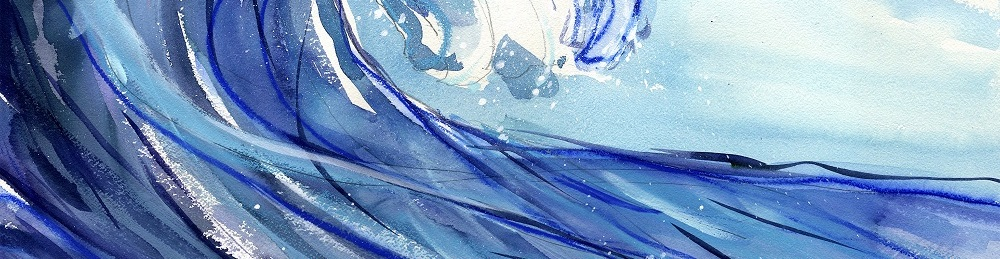
\includegraphics[width=.9\linewidth]{wave-simple}} 

\author{%
\begin{tabular}{c}
	Gabriel Peyr{\'e} \\ CNRS \& DMA \\
	 \'Ecole Normale Sup\'erieure \\
	 \url{gabriel.peyre@ens.fr}\\
	 \url{https://mathematical-tours.github.io}
\end{tabular}
}


\date{\today}

\begin{document}

\maketitle

% !TEX root = ../FundationsDataScience.tex

\chapter*{Presentation}

% \begin{abstract}
	This book draft presents an overview of important mathematical and numerical foundations for modern data sciences. 
	% 
	It covers in particulars the basics of signal and image processing (Fourier, Wavelets, and their applications to denoising and compression), imaging sciences (inverse problems, sparsity, compressed sensing) and machine learning (linear regression, logistic classification, deep learning). 
	%
	The focus is on the mathematically-sounded exposition of the methodological tools (in particular linear operators, non-linear approximation, convex optimization, optimal transport) and how they can be mapped to efficient computational algorithms. 
	%
	These course notes are also intended to be the theoretical companion for the Numerical Tours\footnote{\url{www.numerical-tours.com}} web site, which presents Matlab/Python/Julia/R detailed implementations of all the concepts covered here.
		
% \end{abstract}





\tableofcontents

% !TEX root = ../IntroImaging.tex

\chapter{Claude Shannon and Data Compression}
\label{chap-shannon}

\newcommand{\myfig}[3]{%
\begin{figure}[h!]\centering
#1
\caption{\label{#2}#3}
\end{figure}}

\newcommand{\imgspace}{\hspace{2mm}}
\newcommand{\tabDeux}[1]{%
\begin{tabular}{@{}c@{\imgspace}c@{}}
#1
\end{tabular}}
%
\newcommand{\tabTrois}[1]{%
\begin{tabular}{@{}c@{\imgspace}c@{\imgspace}c@{}}
#1
\end{tabular}}
%
\newcommand{\tabQuatre}[1]{%
\begin{tabular}{@{}c@{\imgspace}c@{\imgspace}c@{\imgspace}c@{}}
#1
\end{tabular}}


\newcommand{\BL}[1]{{\color{blue}{#1}}}
\newcommand{\RE}[1]{{\color{red}{#1}}}
\newcommand{\GR}[1]{{\color{magenta}{#1}}}
\newcommand{\WH}[1]{{\color{white}{#1}}}
\newcommand{\LG}[1]{{\color{lightgray}{#1}}}



\newcommand{\mot}{\BL{v}}
\newcommand{\Mot}{\BL{V}}
\newcommand{\differ}{\GR{d}}
\newcommand{\Differ}{\GR{D}}
%
\newcommand{\LongMoy}{\Ll}
\newcommand{\LongTot}{\bar\Ll}


\newcommand{\mylink}[1]{\footnote{\url{#1}}}



%\newcommand{\myparagraph}[1]{\paragraph{#1.}}
%\renewcommand{\myparagraph}[1]{\subsection{#1}}
 
The vast majority of data (text, sound, image, video, etc.) is stored and manipulated in digital form, that is, using integers which are converted into a succession of bits ($\RE{0}$ and $\RE{1}$). Conversion from the continuous analog world to these discrete numerical representations is described by the theory developed by Claude Shannon (April 30, 1916--February 24, 2001), the founding father of the theory of information. The impact of this theory on our society is absolutely colossal. Yet his name is almost unknown to the general public. The centenary of the birth of Claude Shannon is therefore a good excuse to present the work of a major scientist.


%%%%%%%%%%%%%%%%%%%%%%%%%%%%%%%%%%%%%%%%%%%%%%%%%%%%%%%%%%%%%%%%%%%%%%%%%%%%%%%%%%
%%%%%%%%%%%%%%%%%%%%%%%%%%%%%%%%%%%%%%%%%%%%%%%%%%%%%%%%%%%%%%%%%%%%%%%%%%%%%%%%%%
%%%%%%%%%%%%%%%%%%%%%%%%%%%%%%%%%%%%%%%%%%%%%%%%%%%%%%%%%%%%%%%%%%%%%%%%%%%%%%%%%%
\section{Numeric Data and Coding}

In the digital world that surrounds us, all data (images, films, sounds, texts, etc.) are coded in the form of a succession of $\RE{0}$ and $\RE{1}$. This encoding is not limited to storage on computers, it is also central for communications over the internet (email, \guill{streaming} video, etc.) as well as for applications as diverse as music players, e-readers or mobile phones.

However, data (eg text, sounds, images, or videos) is initially represented as a succession of \textit{symbols}, which are not necessarily $\RE{0}$ or of $\RE{1}$. For example, for the case of a text, the symbols are the letters of the alphabet. For the case of images, these are the values of the pixels. It is therefore necessary to be able to convert this sequence of symbols into a sequence of $\RE{0}$ and $\RE{1}$. It is also necessary to be able to do it in an economical way, that is to say using the shortest possible sequence. This is crucial in order to be able to store this data efficiently on a hard disk, or to transmit them quickly on the Internet. This problem of \textit{compression} has become a major issue because the stored and transmitted data grow exponentially.

The theory developed by Claude Shannon describes the theoretical and algorithmic bases of this coding. He mathematically formalized the three key stages of conversion from the analog world to the digital world:
\begin{itemize}
\item[(i)] \textit{sampling}\mylink{https://en.wikipedia.org/wiki/Sampling_(signal_processing)}, which allows one to switch from continuous data to a succession of numbers;
%
\item[(ii)] \textit{coding}\mylink{https://en.wikipedia.org/wiki/Data_compression} (also known as compression), which allows one to move to a more compact sequence of $\RE{0}$ and $\RE{1}$ (called binary code);
%
\item[(iii)] \textit{error-correcting code}\mylink{https://en.wikipedia.org/wiki/Error_detection_and_correction}, which makes code robust to errors and attacks.
\end{itemize}

For each of these steps, Claude Shannon has established performance \guill{upper bounds} in~\cite{Shannon1948,shannon1949}, under precise assumptions about the data and the transmission channel. These performance bounds set limits that can not be exceeded, regardless of the method used. For example, for the encoding phase (ii), this bound corresponds to the minimum theoretical size of the binary messages making it possible to code the desired information. In the second half of the 20th century, efficient computational methods and algorithms were developed that reach the limits of Shannon, leading to the 21st century on the explosion of the digital age. This article focuses on part (ii) and presents the basics of data compression as defined by Claude Shannon. 

You can find at the end of this article a glossary summarizing the most important terms.


%%%%%%%%%%%%%%%%%%%%%%%%%%%%%%%%%%%%%%%%%%%%%%%%%%%%%%%%%%%%%%%%%%%%%%%%%%%%%%%%%%
%%%%%%%%%%%%%%%%%%%%%%%%%%%%%%%%%%%%%%%%%%%%%%%%%%%%%%%%%%%%%%%%%%%%%%%%%%%%%%%%%%
%%%%%%%%%%%%%%%%%%%%%%%%%%%%%%%%%%%%%%%%%%%%%%%%%%%%%%%%%%%%%%%%%%%%%%%%%%%%%%%%%%
\section{Encoding and Decoding}

We will now describe and study the transformation (coding) from the sequence of $\{\BL{0,1,2,3}\}$ symbols to a binary code, that is, a sequence of $\RE{0}$ and $\RE{1}$.

%%%%%%%%%%%%%%%%%%%%%%%%%%%%%%%%%%%%%%%%%%%%%%%%%% %%%%%%%%%%%%%%%%%%%%%%%%%%%%%%%%
\subsection{Example of an Image}

In the rest of this article, I will illustrate my remarks using grayscale images. Such an image is composed of pixels. To simplify, we will consider only pixels with 4 levels of gray:
\begin{rs}
\item $\BL{0}$: black, 
\item $\BL{1}$: dark gray,
\item $\BL{2}$: light gray,
\item $\BL{3}$: white.
\end{rs}
However, all that will be described hereafter can be generalized to an arbitrary number of gray levels (in general, the images that are found on the Internet have 256 levels) and even to color images (which can be decomposed in 3 monochrome images, the red, green and blue components).

Figure~\ref{fig-image-zoom} shows an example of an image with 4 levels of gray, with a zoom on a subset of $5 \times 5$ pixels.

\myfig{
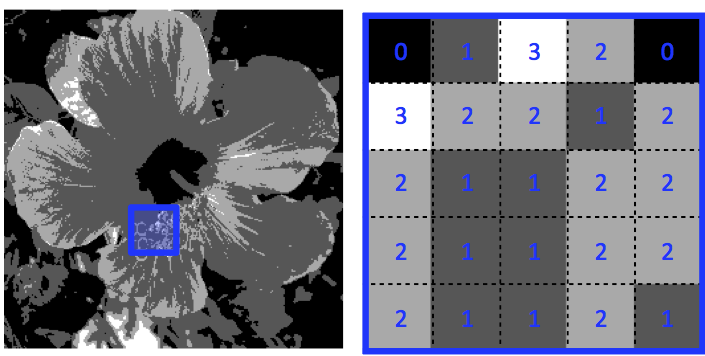
\includegraphics[width=.6\linewidth]{codage/codage-pxl}
}{fig-image-zoom}{A greyscale image and a zoom on a square of $5 \times 5$ pixels}


We will focus on this set of 25 pixels (the rest of the image is treated in the same way). If we put the corresponding values one after the other, we get the following sequence of symbols, which are numbers between $\BL{0}$ and $\BL{3}$
$$
	(\BL{0, 1, 3, 2, 0, 3, 2, 2, 1, 2, 2, 1, 1, 2, 2, 2, 1, 1, 2, 2, 2, 1, 1, 2, 1}).
$$

%%%%%%%%%%%%%%%%%%%%%%%%%%%%%%%%%%%%%%%%%%%%%%%%%% %%%%%%%%%%%%%%%%%%%%%%%%%%%%%%%%
\subsection{Uniform Coding}

The coding step therefore proceeds by associating to each of the symbols $\{\BL{0,1,2,3}\}$ a code word, which is a sequence of $\RE{0}$ and $\RE{1}$.

One possible strategy is to use coding
$$
\BL{0} \mapsto \RE{00}, \quad
\BL{1} \mapsto \RE{01}, \quad
\BL{2} \mapsto \RE{10}, \quad
\BL{3} \mapsto \RE{11}.
$$
This is a particular case of \textit{uniform} coding, which associates with each symbol a code word of fixed length (here of constant length 2).

Thus the sequence of $(\BL{0, 1, 3})$ symbols is coded as
$$
	(\BL{0, 1, 3}) \overset{\text{coding}}{\longmapsto}
	(\RE{00,01,11}) \overset{\text{grouping}}{\longmapsto}
	\RE{000111}.
$$
The complete sequence of symbols corresponding to the image of $5 \times 5$ pixels shown above
will give the code
$$
  \RE{00011110001110100110100101101010010110101001011001}.
$$
The length (ie the number of $\BL{0}$ and $\BL{1}$) in the sequence $\BL{0}$ and $\BL{1}$ used to encode a message is measured in number of \textit{bits}. Using the previous uniform coding, which uses 2 bits per symbols, as one must code 25 symbols, a length
$$
	\mathcal{\bar L} = 25 \times 2 = 50 \text{ bits}
$$
The \textit{bit} (\guill{binary digit}) is the fundamental unit of information, and was introduced by John Tukey\mylink{https://en.wikipedia.org/wiki/John_Tukey} who was a collaborator of Claude Shannon.



%%%%%%%%%%%%%%%%%%%%%%%%%%%%%%%%%%%%%%%%%%%%%%%%%% %%%%%%%%%%%%%%%%%%%%%%%%%%%%%%%%
\subsection{Logarithm and Uniform Coding}

If the number $N$ of possible symbols (in this case $N=4$) is a power of $2$, that is $N=2^\ell$ (here $N=4=2^2$ so that $\ell=2$), one can always construct such a \textit{uniform} code where one associates to each symbol its binary writing. We have given the example of the uniform coding of $N=4$ symbols, and the case of $N=8$  (thus $\ell=3$) symbols corresponds to the coding
$$
\BL{0} \mapsto \RE{000}, \quad
\BL{1} \mapsto \RE{001}, \quad
\BL{2} \mapsto \RE{010}, \quad
\BL{3} \mapsto \RE{011},
$$
$$
\BL{4} \mapsto \RE{100}, \quad
\BL{5} \mapsto \RE{101}, \quad
\BL{6} \mapsto \RE{110}, \quad
\BL{7} \mapsto \RE{111}.
$$

This binary code has a length $\ell$, which is called the logarithm in base of 2\mylink{https://en.wikipedia.org/wiki/Binary_Logarithm} of $N$, which is noted
$$
	N=2^\ell \quad \Longleftrightarrow \quad \log_2(N) \eqdef \ell.
$$
The definition of $\log_2(x)$ also extends to the case where $x$ is not a power of 2, using the definition $\log_2(x) \eqdef \ln(x)/\ln(2)$, where $\ln$ is the \textit{natural logarithm}.
%
In this case, $\log_2(x)$ is not an integer. For a strictly positive real number $x$, the logarithm satisfies
$\log_2(1/x)=-\log_2(x)$, so for example, we have $\log_2(1/4)=-\log_2(4)=2$.



%%%%%%%%%%%%%%%%%%%%%%%%%%%%%%%%%%%%%%%%%%%%%%%%%%%%%%%%%%%%%%%%%%%%%%%%%%%%%%%%%%
\subsection{Variable-length Encoding}

An important question is whether we can do better (that is, use fewer bits to code the same sequence of symbols). For example, the following coding may be used instead of a uniform code
$$
\BL{0} \mapsto \RE{001}, \quad
\BL{1} \mapsto \RE{01}, \quad
\BL{2} \mapsto \RE{1}, \quad
\BL{3} \mapsto \RE{000}.
$$
With such coding, the $(\BL{0, 1, 3})$ symbol sequence is coded as
$$
	(\BL{0, 1, 3}) \overset{\text{codage}}{\longmapsto}
	(\RE{001,01,000}) \overset{\text{regroupement}}{\longmapsto}
	\RE{00101000}.
$$
The complete sequence of symbols corresponding to the image of $5 \times 5$ pixels
will give the code
$$
  \RE{001010001001000110111010111101011110101101}.
$$
The length of the binary code obtained is therefore now
$$
	\mathcal{\bar L} = 42 \text{bits}
$$
This shows that it is therefore possible to do better than with a \textit{uniform} coding using a \textit{variable} coding, which associates a variable length code with each symbol.

It is also possible to define the average number of bits per symbol $\mathcal{L}$, which is computed, here for a sequence of 25 symbols, as
$$
	\mathcal{L} \eqdef \frac{ \mathcal{\bar L} }{25} = \frac{42}{25} = 1.68 \text{ bits.}
$$
Compared to a uniform coding, it is seen that the average number of bits per symbol has changed from $\log_2(N)=2 \text{ bits}$ to $ 1.68 \text{ bits}$.




%%%%%%%%%%%%%%%%%%%%%%%%%%%%%%%%%%%%%%%%%%%%%%%%%% %%%%%%%%%%%%%%%%%%%%%%%%%%%%%%%%
\subsection{Prefix Coding and Decoding}

These codings, uniform or of variable length, would be of no interest if we did not ensure that the message obtained is \textit{decodable}, ie we can find the sequence of symbols at the origin of a binary code. All encodings do not allow for this reverse path.

For uniform encodings, such as coding
$$
\BL{0} \mapsto \RE{00}, \quad
\BL{1} \mapsto \RE{01}, \quad
\BL{2} \mapsto \RE{10}, \quad
\BL{3} \mapsto \RE{11}.
$$
it is sufficient to separate the sequence of bits into packets of length $\log_2(N)$(here $ N=$ 4 and $\log_2(N)=$ 2) and use the encoding table in the opposite direction.
Thus, the $\RE{000111}$ binary code is decoded as
$$
	\RE{000111} \overset{\text{splitting}}{\longmapsto}
	(\RE{00,01,11})  \overset{\text{decoding}}{\longmapsto}
	(\BL{0, 1, 3}).
$$

On the other hand, if we consider the coding
$$
\BL{0} \mapsto \RE{0}, \quad
\BL{1} \mapsto \RE{10}, \quad
\BL{2} \mapsto \RE{110}, \quad
\BL{3} \mapsto \RE{101},
$$
then the bit sequence $\RE{1010}$ can be decoded in two ways:
$$
	\RE{1010}
	\overset{\text{splitting}}{\longmapsto}
	(\RE{10, 10})
	\overset{\text{decoding}}{\longmapsto}
	(\BL{1, 1}),
$$
or
$$
	\RE{1010}
	\overset{\text{splitting}}{\longmapsto}
	(\RE{101, 0})
	\overset{\text{decoding}}{\longmapsto}
	(\BL{3, 0}).
$$
This means that this sequence can be decoded either as the sequence $(\BL{1, 1})$, or as the $(\BL{3, 0})$ sequence.
Note that the $\RE{10}$ encoding word used to encode $\BL{1}$ is the beginning of the $\RE{101}$ word used to encode $\BL{3}$.

To be able to do the decoding in an unambiguous way, it is enough that no word of the coding is the beginning of another word. When this condition is satisfied, we speak of \textit{prefix}\mylink{https://en.wikipedia.org/wiki/Prefix_Code}
and it is therefore possible to carry out the decoding step by step.
It is easily verified that this is indeed the case for the non-uniform coding already considered previously
$$
\BL{0} \mapsto \RE{001}, \quad
\BL{1} \mapsto \RE{01}, \quad
\BL{2} \mapsto \RE{1}, \quad
\BL{3} \mapsto \RE{000}.
$$
The progressive decoding of the symbol message of the pixels of the image is carried out as follows:
$$
	\RE{001}\LG{010001001000110111010111101011110101101}
		\longrightarrow  \text{ decoding } \BL{0}
$$
$$
	\WH{0}\BL{0}\WH{1}\RE{01}\LG{0001001000110111010111101011110101101}
			\longrightarrow  \text{ decoding } \BL{1}
$$
$$
	\WH{0}\BL{0}\WH{1}\BL{1}\WH{0}\RE{000}\LG{1001000110111010111101011110101101}
	\longrightarrow  \text{ decoding } \BL{3}
$$
$$
	\WH{0}\BL{0}\WH{1}\BL{1}\WH{0}\WH{0}\BL{3}\WH{0}\RE{1}\LG{001000110111010111101011110101101}
		\longrightarrow  \text{ decoding } \BL{2} \ldots
$$

%%%%%%%%%%%%%%%%%%%%%%%%%%%%%%%%%%%%%%%%%%%%%%%%%% %%%%%%%%%%%%%%%%%%%%%%%%%%%%%%%%
\subsection{Codes and Trees}
\label{sec-arbres}

As shown in Figure~\ref{fig-trees}, in the top left, it is possible to place the set of binary codes of less than $\ell $ bits in a tree of depth $\ell + 1 $. The $ 2^\ell $ words of length exactly $\ell $ occupy the sheets, and the shorter words are the inner nodes.

\myfig{
\tabTrois{
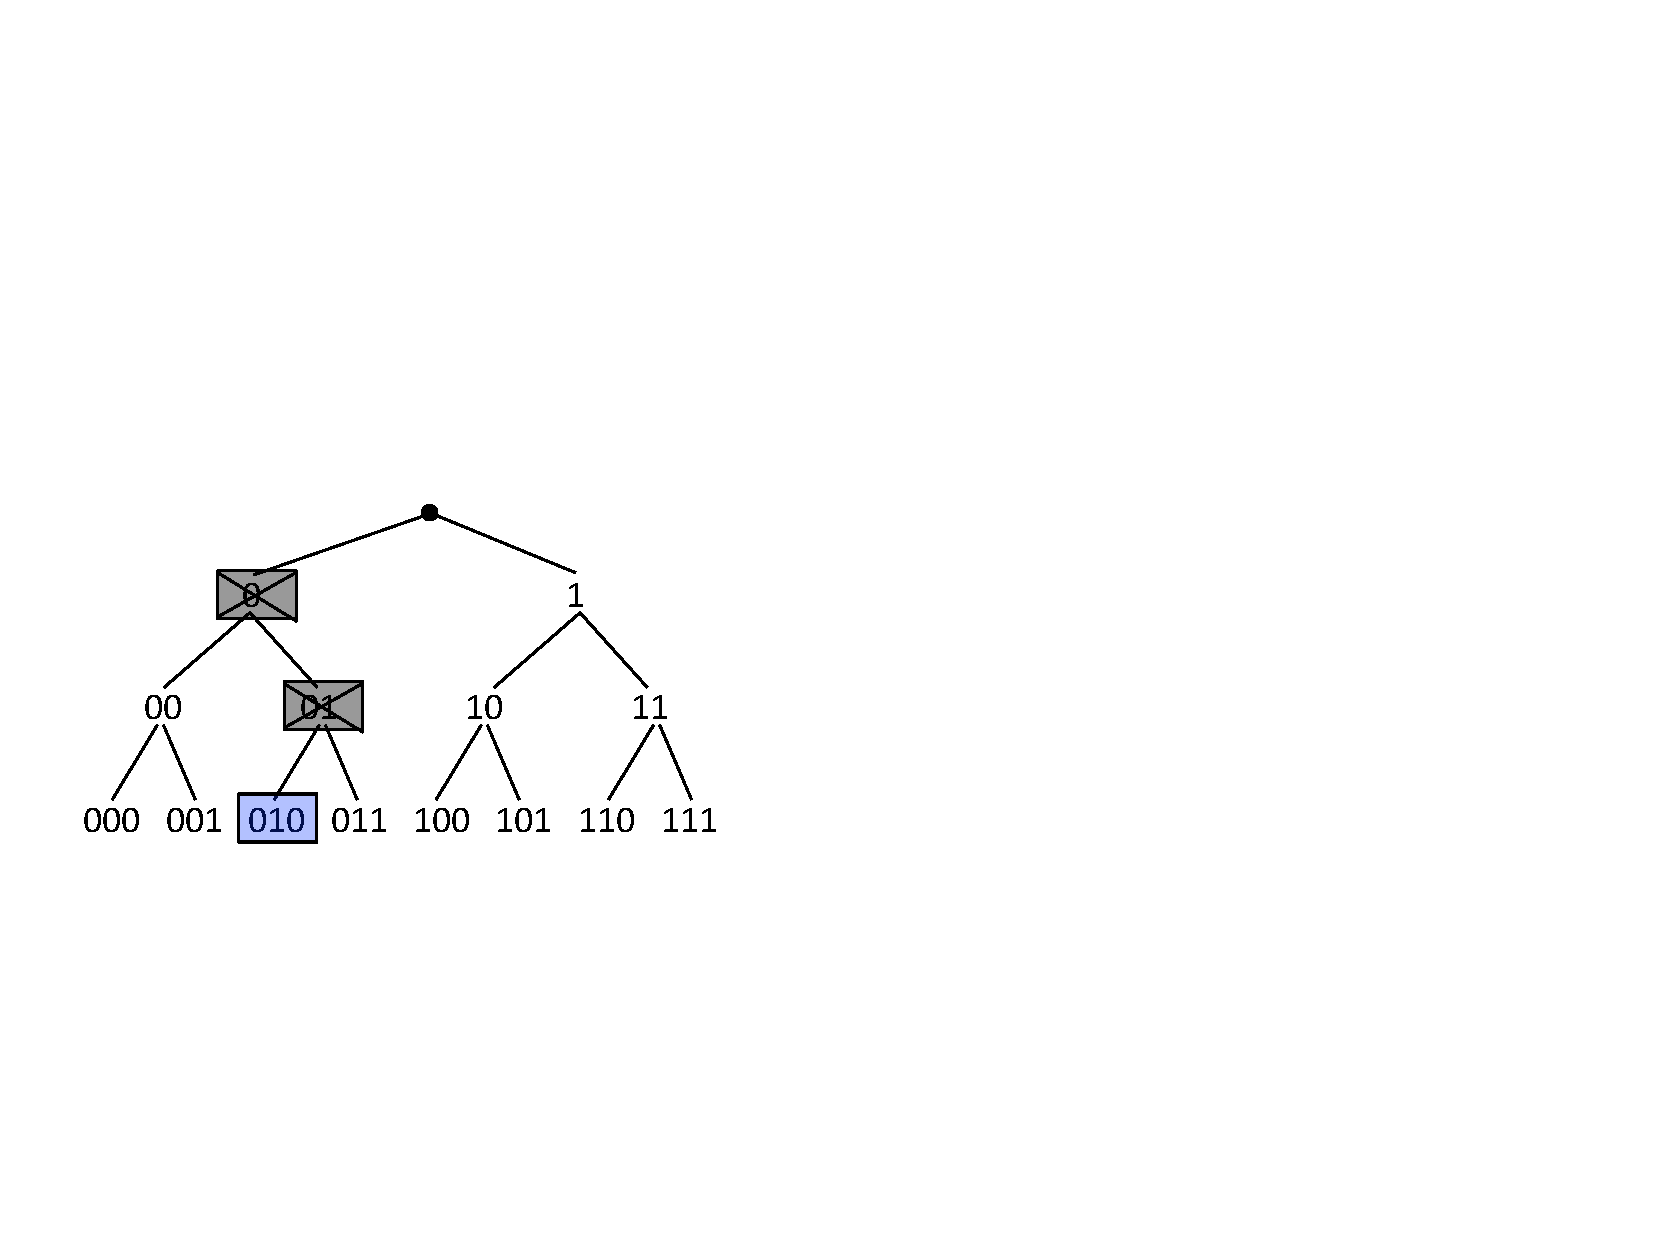
\includegraphics[width=.45\linewidth]{arbres/codage-prefixe}&
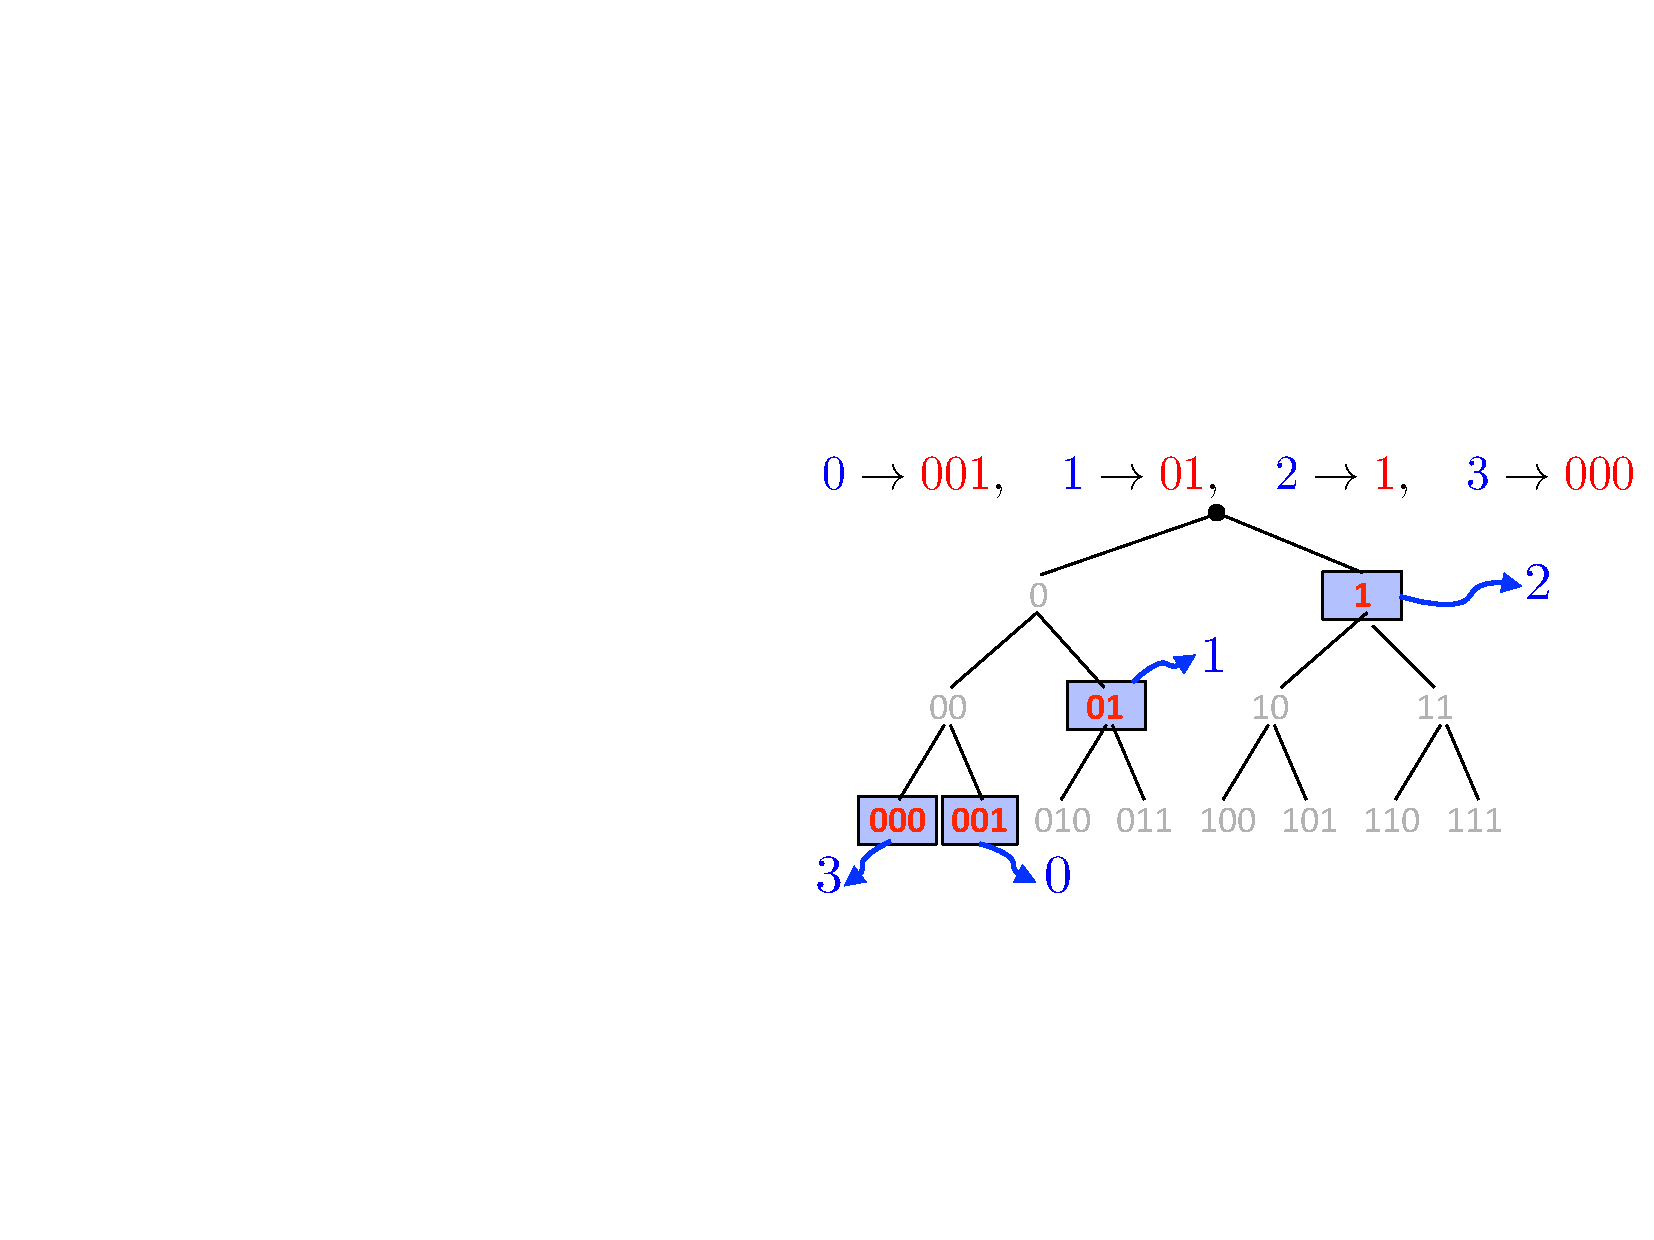
\includegraphics[width=.45\linewidth]{arbres/arbre-exemple}
}
}{fig-trees}{Left: complete tree of all codes of length 3; right: example of prefix code.}

The prefix encodings are then represented as the leaves of the subtrees of this complete tree. Figure~\ref{fig-trees}, top right, shows which subtree corresponds to the variable-length code
$$
\BL{0} \mapsto \RE{001}, \quad
\BL{1} \mapsto \RE{01}, \quad
\BL{2} \mapsto \RE{1}, \quad
\BL{3} \mapsto \RE{000}.
$$
Once a prefix encoding has been represented as a binary subtree, the decoding algorithm is particularly simple to implement. When decoding is begun, one moves to the root, and descends to each new bit read either to the left (for a $\RE{0}$) or to the right (for a $\RE{1}$). When one reaches a leaf of the subtree, one then sends the word of the code corresponding to this leaf, and one restarts to the root. The previous figure shows the decoding process.


%%%%%%%%%%%%%%%%%%%%%%%%%%%%%%%%%%%%%%%%%%%%%%%%%% %%%%%%%%%%%%%%%%%%%%%%%%%%%%%%%%
%%%%%%%%%%%%%%%%%%%%%%%%%%%%%%%%%%%%%%%%%%%%%%%%%% %%%%%%%%%%%%%%%%%%%%%%%%%%%%%%%%
%%%%%%%%%%%%%%%%%%%%%%%%%%%%%%%%%%%%%%%%%%%%%%%%%% %%%%%%%%%%%%%%%%%%%%%%%%%%%%%%%%
\section{The Shannon Bound}

After describing the coding techniques, we will now explain the Shannon theory, which analyzes the performance of these techniques (ie the number of bits needed for coding) by performing a random modeling of the message to be coded which is composed of a particular sequence of symbols).


%%%%%%%%%%%%%%%%%%%%%%%%%%%%%%%%%%%%%%%%%%%%%%%%%% %%%%%%%%%%%%%%%%%%%%%%%%%%%%%%%%
\subsection{Minimum Length Code and Random Modeling}

The use of variable length prefix encoding shows that an average number of bits $\mathcal{L}$can be obtained than the number $\log_2(N)$ of bits obtained by a uniform code. The fundamental question, both on a theoretical and practical level, is whether we can find a prefix coding giving rise to a minimum number of bits per symbol.

This question is not correctly phrased, because its answer depends on the message to be coded, and this message is generally unknown a priori. A model is therefore needed to describe possible messages. The fundamental idea introduced by Claude Shannon is to use a probabilistic model: we do not know what messages we will have to code, but we assume that we know the probability of appearance of the symbols composing this message.

Shannon assumes that the symbols that make up the modeled message are drawn \textit{independently}\mylink{https://en.wikipedia.org/wiki/Independencies_(probability)}
according to a random variable $\Mot$(the source of the message). This means that the symbols composing the modeled message are independent random variables with the same distribution as $\Mot$.

%%%%%%%%%%%%%%%%%%%%%%%%%%%%%%%%%%%%%%%%%%%%%%%%%% %%%%%%%%%%%%%%%%%%%%%%%%%%%%%%%%
\subsection{Empirical Frequencies}

In order to apply this probabilistic model to a given message, we will act as if we randomly draw each symbol one after the other according to probabilities identical to the frequencies observed (on average) in the case studied.

This means that we impose that the distribution of the $\Mot$ source to be equal to the empirical frequencies observed in the message.
%
Empirical frequencies $(p_{\BL{0}},p_{\BL{1}},p_{\BL{2}},p_{\BL{3}})$ are the frequency of appearance of the different symbols $(\BL{0,1,2,3})$. 
%
For the set of the 25 pixels of the grayscale image
$$
	(\BL{0, 1, 3, 2, 0, 3, 2, 2, 1, 2, 2, 1, 1, 2, 2, 2, 1, 1, 2, 2, 2, 1, 1, 2, 1}), 
$$
the frequency $p_{\BL{1}}$ is equal to $ 9/25 $ because the symbol $\BL{1}$ appears $ 9 $ times and it is desired to encode a sequence of 25 symbols. The list of empirical frequencies for this sequence of symbols is thus
$$
  	p_{\BL{0}} = \tfrac{2}{25}, \quad
	p_{\BL{1}} = \tfrac{9}{25}, \quad
	p_{\BL{2}} = \tfrac{12}{25}, \quad
	p_{\BL{3}} = \tfrac{2}{25}.
$$

The random modeling therefore imposes on the variable $\Mot$ to have for probability distribution $(p_{\BL{0}},p_{\BL{1}},p_{\BL{2}},p_{\BL{3}})$, ie the probability that a symbol of the modeled message (assumed to be generated by the $\Mot$ source) is $\mathbb{P}(\Mot=\mot) = p_{\mot}$.

This is an important example of modeling, which is of course not always relevant but allows a fine analysis of the problem. For example, in the case of an image, if a pixel is black, the next one is likely to be black, even if the overall black frequency is low. This defeats the independence hypothesis (the \guill{Information Transformation} section details this example).


%%%%%%%%%%%%%%%%%%%%%%%%%%%%%%%%%%%%%%%%%%%%%%%%%% %%%%%%%%%%%%%%%%%%%%%%%%%%%%%%%%
\subsection{Entropy} 

In order to answer the coding problem with a minimum average number of bits, Shannon introduced a fundamental mathematical object: \textit{entropy}\mylink{https://en.wikipedia.org/wiki/Entropy}.
Entropy was invented by Ludwig Boltzmann\mylink{https://en.wikipedia.org/wiki/Ludwig_Boltzmann}
in the context of thermodynamics\mylink{https://en.wikipedia.org/wiki/Entropie_(thermodynamics)}
and this concept was taken up by Claude Shannon to develop his theory of information.
The entropy of the distribution of the source $\Mot$ is defined by the formula
$$
	\mathcal{H}_\Mot \eqdef -\sum_{\mot=0}^{N-1} p_{\mot} \times \log_2(p_{\mot}).
$$
This formula means that we sum up for all possible $\mot$ symbols the frequency of occurrence $p_{\mot}$ of the symbol $\mot$ multiplied by the logarithm $\log_2(p_{ \mot})$ of this frequency, then take the opposite (minus sign) of the number obtained.

As the logarithm is an increasing function, and as $\log_2(1)=0$, we have $\log_2(p_{\mot}) \leq 0$ because $p_{\mot}$ is always less than $1$). The minus sign before the formula defining the entropy ensures that this quantity is always positive.

In our case, we have $N=4$ values for the symbols, and we use the formula
$$
	\mathcal{H}_\Mot \eqdef
- p_{\BL{0}} \times \log_2(p_{\BL{0}})
- p_{\BL{1}} \times \log_2(p_{\BL{1}})
- p_{\BL{2}} \times \log_2(p_{\BL{2}})
- p_{\BL{3}} \times \log_2(p_{\BL{3}}).
$$
Note that if $p_{\mot}=0$, then the convention $p_{\mot} \times \log_2(p_{\mot})=0 \times \log_2(0)=$ 0. This convention means that null probabilities (ie, impossible events) are not taken into account in this formula. Moreover, it is consistent with the limit value of the function $x \mapsto x \ln(x)$ at $x=0$.



The goal of entropy is to quantify the uncertainty on possible symbol sequences generated by the $\Mot$ source. We can show that the entropy verifies
$$
	0 \leq \mathcal{H}_\Mot \leq \log_2(N).
$$
The two extreme values thus correspond to respective minimum and maximum uncertainties.

\myfig{
\tabQuatre{
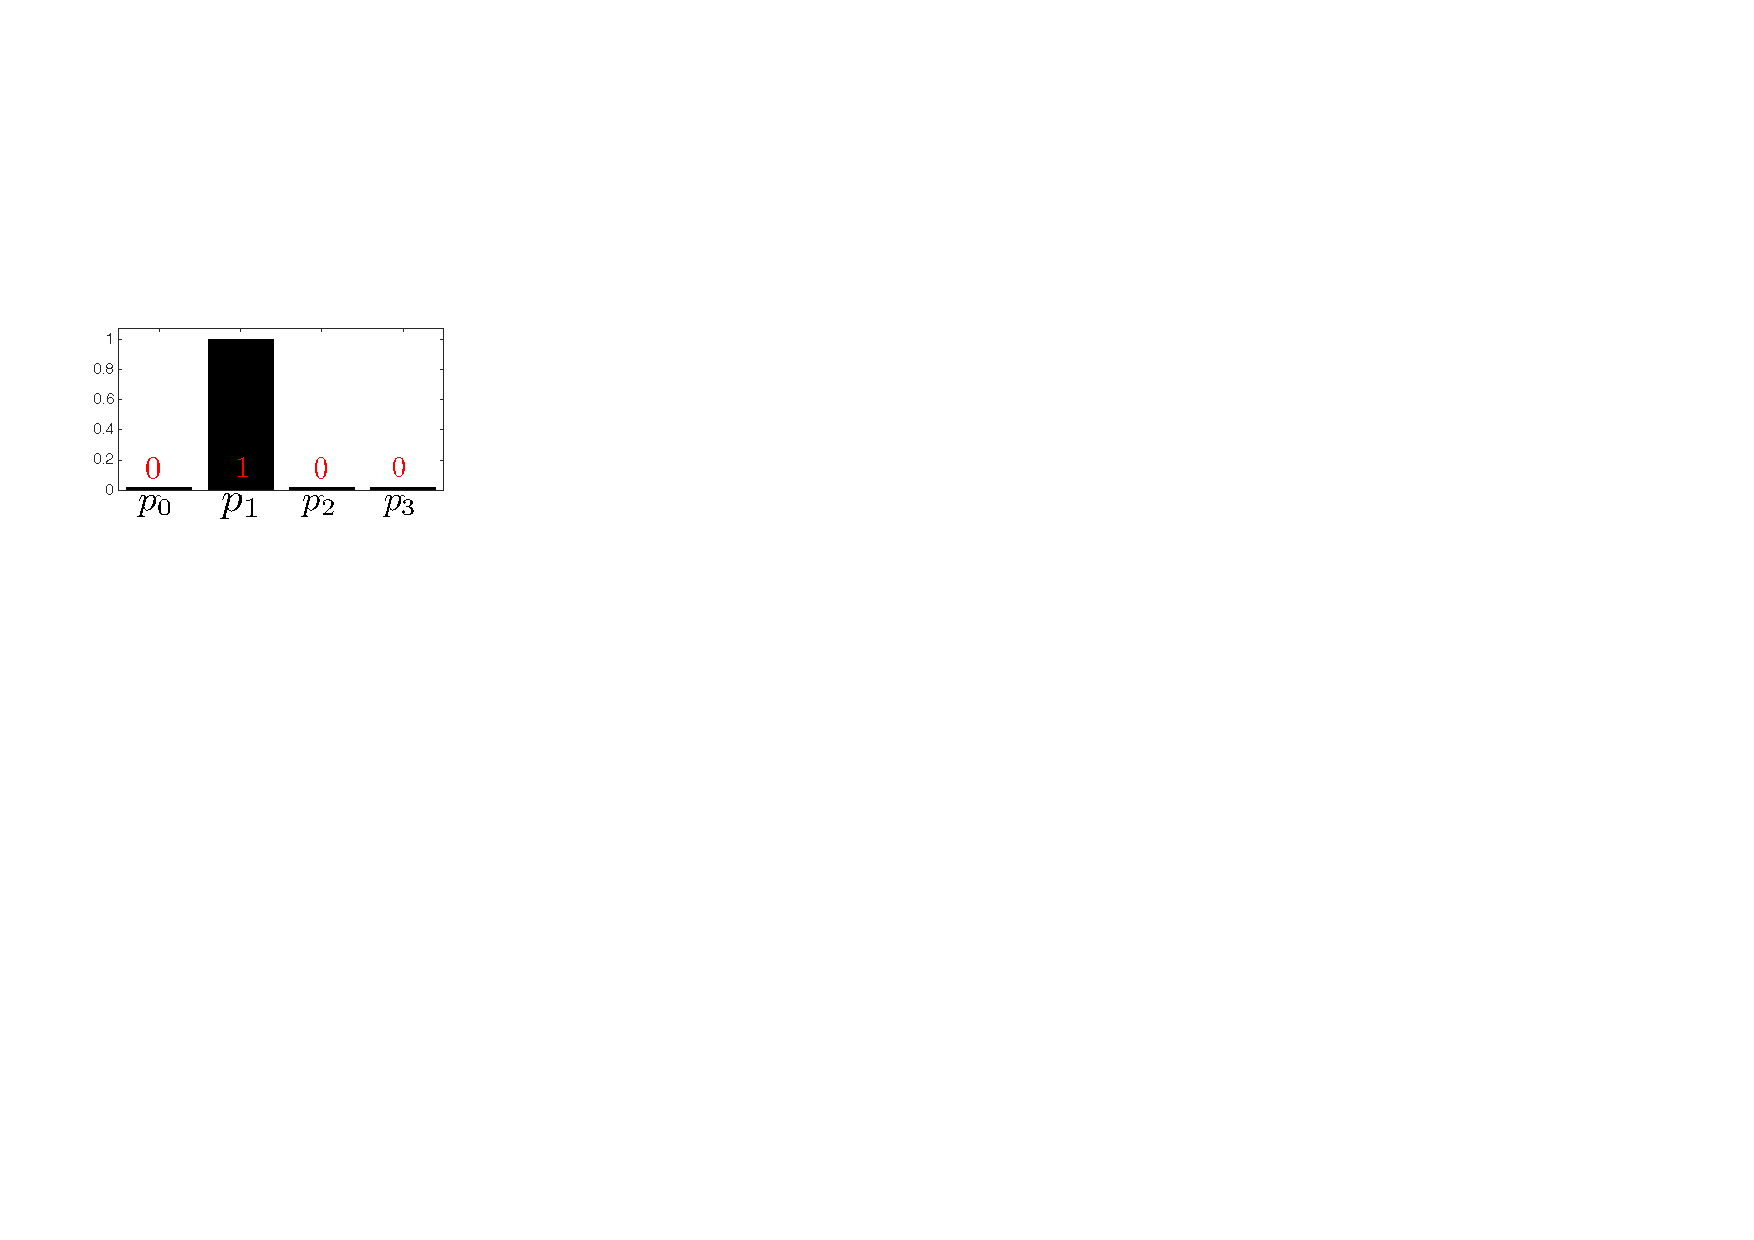
\includegraphics[width=.3\linewidth]{entropie/histo-1}&
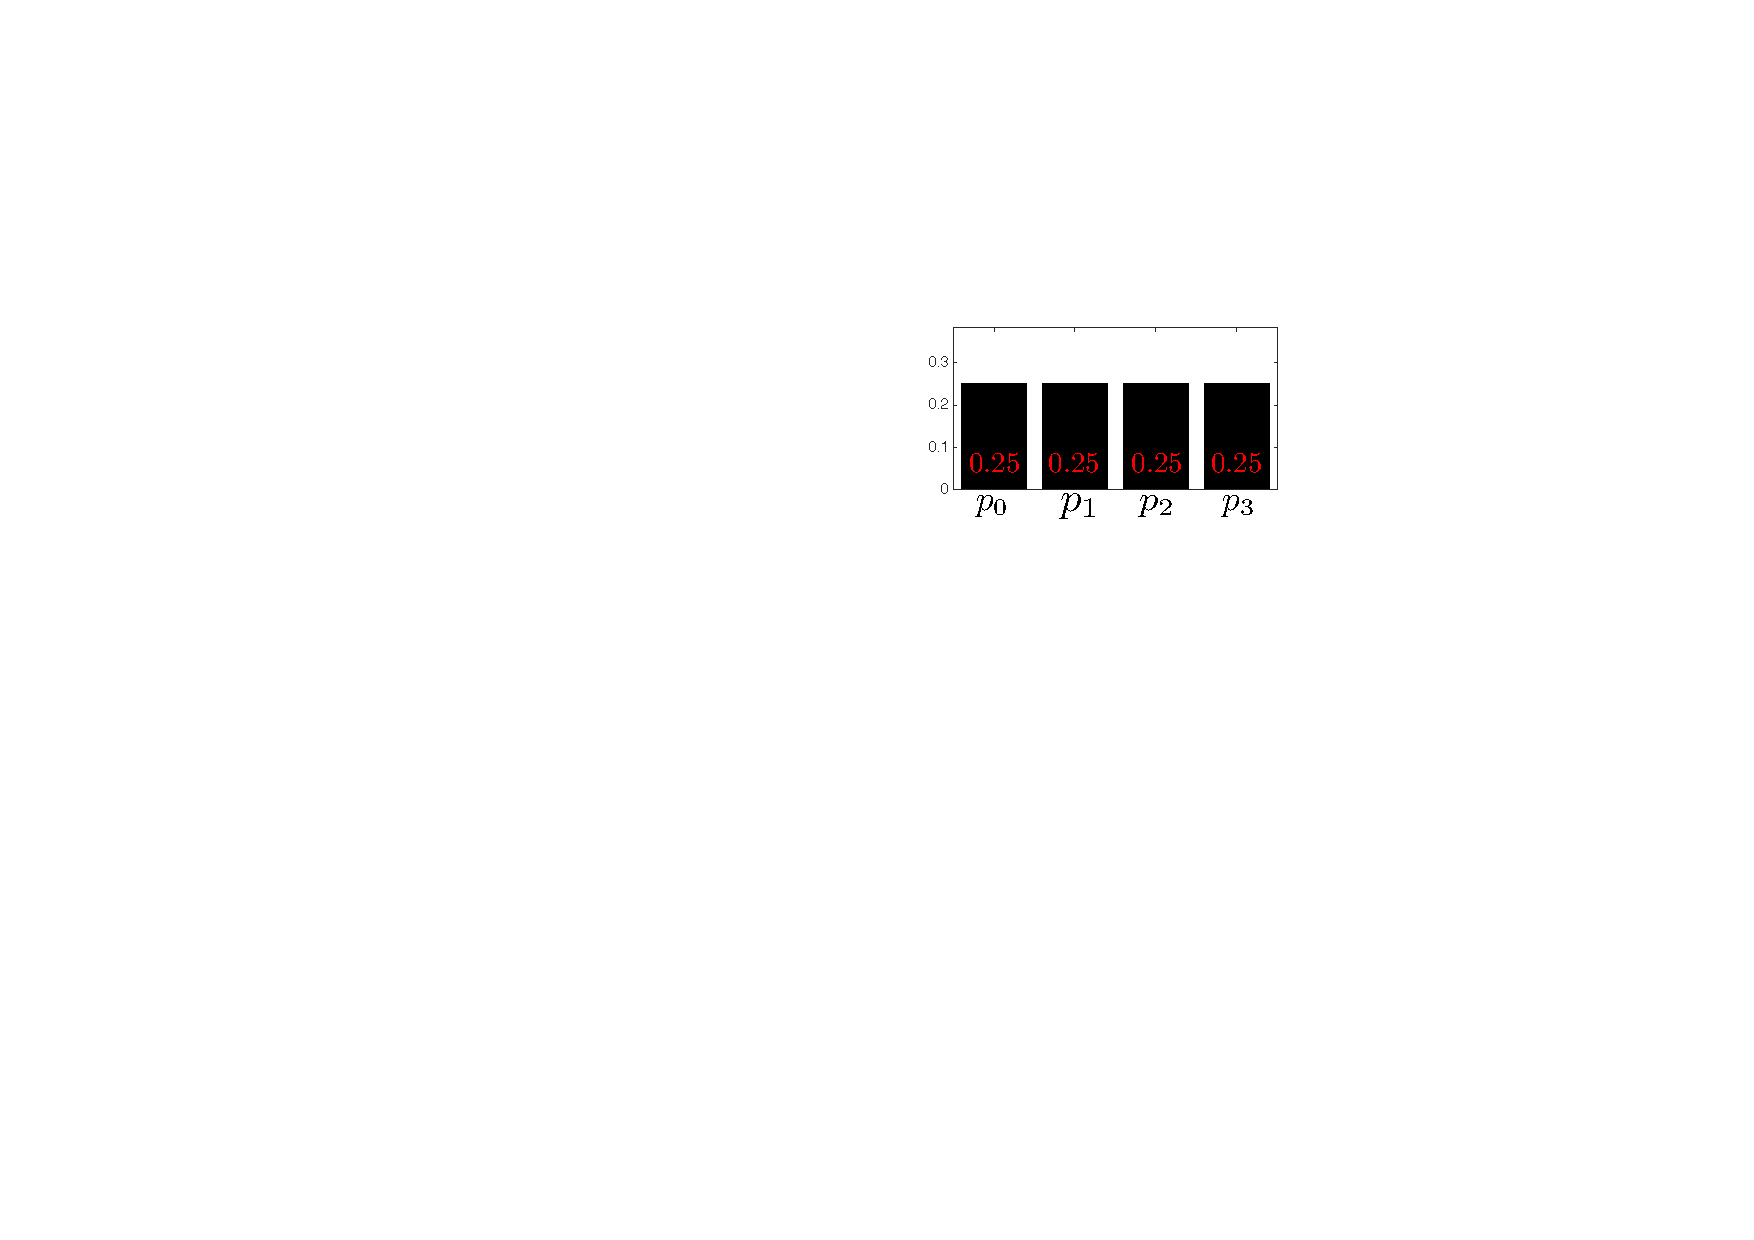
\includegraphics[width=.3\linewidth]{entropie/histo-3}&
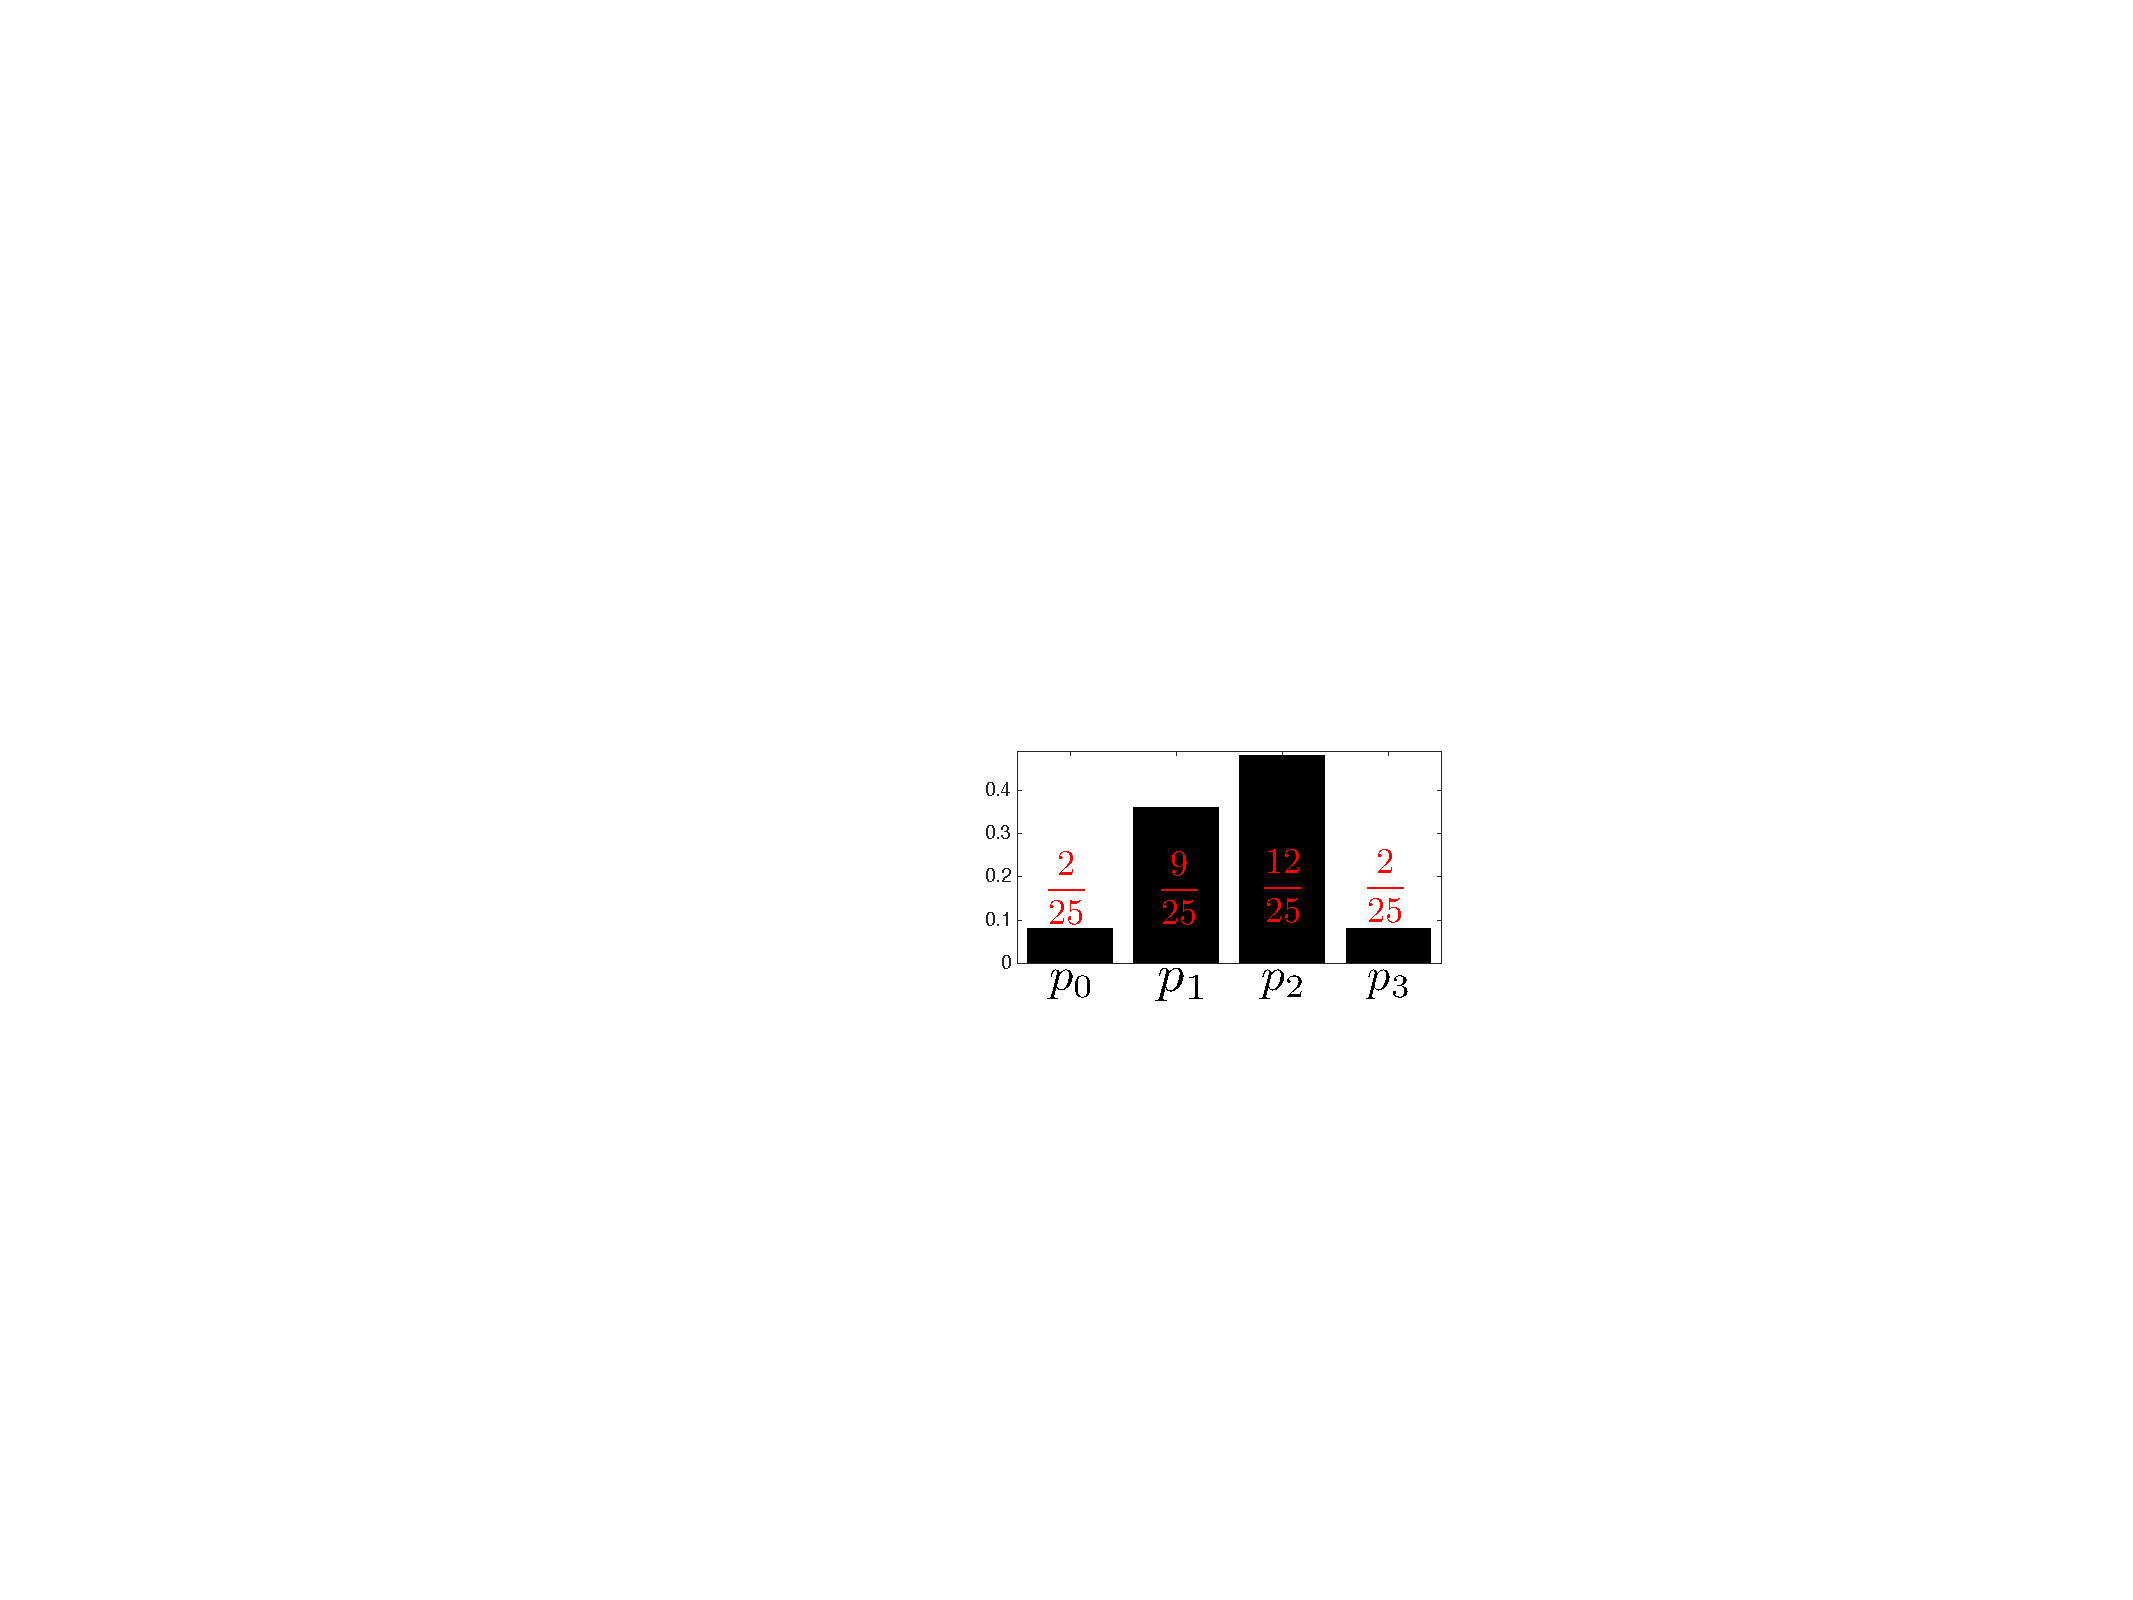
\includegraphics[width=.3\linewidth]{entropie/histo-sub}\\
$\Hh_{\Mot}=0$ & $\Hh_{\Mot}=\log_2(2)=1$ &  $\Hh_{\Mot} = 1.62$
}
}{fig-histo-entropy}{Three examples of probability distributions with corresponding entropies.}


\begin{itemize}
%%%%%%%%%%%%%%%%%%%%%%%%%%%%%%%%%%%%%%%%%%%%%%%%%%%%%%%%%%%%%%%%%%%%
\item \textbf{Minimal entropy}
%
 The entropy $\mathcal{H}_\Mot=0$  is minimal when the frequencies $p_{\mot}$ are all null except one. The left-handed figure~\ref{fig-histo-entropy} shows the case where $p_{\BL{1}}=1$ and all other probabilities are null.


In this case,
$$
	\mathcal{H}_\Mot = - 0 \times \log_2(0) - 1 \times \log_2(1) - 0 \times \log_2(0)- 0 \times \log_2(0) = 0, 
$$
where we recall that $\log_2(1)=0$ and that by convention we have $ 0 \times \log_2(0)=0$.
This corresponds to the modeling of a constant sequence of symbols, and the source will generate, for example, with probability 1 the following sequence of 25 symbols
$$
		(\BL{0, 0, 0, 0, 0, 0, 0, 0, 0, 0, 0, 0, 0, 0, 0, 0, 0, 0, 0, 0, 0, 0, 0, 0, 0}).
$$
%%%%%%%%%%%%%%%%%%%%%%%%%%%%%%%%%%%%%%%%%%%%%%%%%%%%%%%%%%%%%%%%%%
\item \textbf{Maximum entropy}
%
On the other hand, $\mathcal{H}_\Mot=\log_2(N)$ is maximal when all frequencies are equal, $p_{\mot}=1/N $.
In our case where $N=4$, we have
$$
 \mathcal{H}_\Mot =
 		-\tfrac{1}{4} \times \log_2(\tfrac{1}{4})
  	-\tfrac{1}{4} \times \log_2(\tfrac{1}{4})
		-\tfrac{1}{4} \times \log_2(\tfrac{1}{4})
		-\tfrac{1}{4} \times \log_2(\tfrac{1}{4})
		= \log_2(4) = 2,
$$
where $\log_2(1/x)=-\log_2(x)$ is used and therefore in particular $\log_2(\frac{1}{4})=-\log_2(4)$. The following figure~\ref{fig-histo-entropy}, center, shows the histogram corresponding to this case.

This situation corresponds intuitively to the modeling of a sequence maximally \textit{uncertain}.
Here, for example, are two sequences of symbols generated by such a source $\Mot$
$$
  (\BL{2, 2, 1, 1, 3, 0, 3, 3, 3, 0, 1, 1, 2, 0, 2, 0, 2, 1, 3, 2, 0, 2, 2, 1, 3}),
$$
$$
  (\BL{3, 3, 1, 2, 0, 0, 2, 2, 1, 3, 2, 2, 3, 3, 2, 0, 0, 3, 0, 1,  3, 0, 1, 1, 2}).
$$

%%%%%%%%%%%%%%%%%%%%%%%%%%%%%%%%%%%%%%%%%%%%%%%%%%%%%%%%%%%%%%%%%%
\item \textbf{Intermediate entropy}
%
The intermediate situations between these two extremes correspond to intermediate entropies.
For example, we can consider the distribution of the 25 pixels considered at the beginning of this article, which correspond to the message
$$
	(\BL{0, 1, 3, 2, 0, 3, 2, 2, 1, 2, 2, 1, 1, 2, 2, 2, 1, 1, 2, 2, 2, 1, 1, 2, 1}).
$$
For this distribution, we recall that we have the probabilities
$$
  p_{\BL{0}} = \tfrac{2}{25}, \quad
	p_{\BL{1}} = \tfrac{9}{25}, \quad
	p_{\BL{2}} = \tfrac{12}{25}, \quad
	p_{\BL{3}} = \tfrac{2}{25},
$$
the figure~\ref{fig-histo-entropy}, right, shows the histogram corresponding to these values.


The entropy then
$$
	\mathcal{H}_\Mot =
	  -\tfrac{2}{25} \times \log_2(\tfrac{2}{25})
		-\tfrac{9}{25} \times \log_2(\tfrac{9}{25})
		-\tfrac{12}{25}\times \log_2(\tfrac{12}{25})
		-\tfrac{2}{25}\times \log_2(\tfrac{2}{25}) \approx 1.62,
$$
which corresponds to a \guill{intermediate} value of the entropy.
\end{itemize}


%%%%%%%%%%%%%%%%%%%%%%%%%%%%%%%%%%%%%%%%%%%%%%%%%% %%%%%%%%%%%%%%%%%%%%%%%%%%%%%%%%
\subsection{Average number of bits of a source}

In the following, we denote $c_{\mot}$ the code associated with a symbol $\mot$. The length (i.e. the number of bits) of each word $c_{\mot}$ of code is denoted $L(c_{\mot})$. For uniform coding, then the length is constant $L(c_{\mot})=\log_2(N)$.
On the other hand, if we take the example of variable coding
$$
	\BL{0} \mapsto c_{\BL{0}} \eqdef \RE{001}, \quad
	\BL{1} \mapsto c_{\BL{1}} \eqdef \RE{01}, \quad
	\BL{2} \mapsto c_{\BL{2}} \eqdef \RE{1}, \quad
	\BL{3} \mapsto c_{\BL{3}} \eqdef \RE{000},
$$
then $L(c_{\BL{0}})=L(\RE{001})=$ 3.

It can be seen that the average bit number $\mathcal{L}$ of the encoding of a message can be calculated using the empirical frequencies as follows:
$$
	\mathcal{L} = \sum_{\mot=0}^{N-1} p_{\mot} \times L(c_{\mot}).
$$
This formula means that we sum up for all possible $\mot$ symbols the frequency of occurrence $p_{\mot}$ of the symbol multiplied by the length $L(c_{\mot})$ of the code word $c_{\mot}$. For example, in our case, for $ N=$ 4, we have the formula
$$
	\mathcal{L} =
		p_{\BL{0}} \times L(c_{\BL{0}}) +
		p_{\BL{1}} \times L(c_{\BL{1}}) +
		p_{\BL{2}} \times L(c_{\BL{2}}) +
		p_{\BL{3}} \times L(c_{\BL{3}}).
$$
As part of the random modeling using a $\Mot$ source, we will write $\mathcal{L}_\mot$ this average bit number, which is associated with the source $\Mot$ having the distribution $(p_\mot)_{\mot}$.


%%%%%%%%%%%%%%%%%%%%%%%%%%%%%%%%%%%%%%%%%%%%%%%%%% %%%%%%%%%%%%%%%%%%%%%%%%%%%%%%%%
\subsection{Shannon Bound for Coding}

Claude Shannon showed in his article~\cite{Shannon1948} that the entropy allows to bound the average number of bits $\mathcal{L}_\mot$ within the framework of this random model. He indeed showed that for any prefix encoding, one has
$$
	\mathcal{H}_\Mot \leq \mathcal{L}_\mot.
$$
This is a lower bound, and it says no prefix encoding can do better than this bound.

This result is fundamental because it describes an unbreakable limit, whatever the prefix encoding technique used. Its proof is too difficult to be exposed here, it uses the representation in the form of a tree detailed above in Section~\ref{sec-arbres}, one can look for example~\cite{mallat2009a-wav} for the details. This proof shows that it is necessary to spend on average at least $-\log_2(p_{\mot})$ bits (which is, as we have already seen, always a positive number) to code a symbol $\mot$ if one wants to have an effective coding. The most frequent symbols need fewer bits because $p_{\mot}$ is smaller, so the optimal length $-\log_2(p_{\mot})$ is also smaller. This is very natural, as can be seen in particular for the two extreme cases:

\begin{itemize}
%%%%%%%%%%%%%%%%%%%%%%%%%%%%%%%%%%%%%%%%%%%%%%%%%%%%%%%%%%%%%%%%%%
\item \textbf{Minimal entropy}
%
If $\mathcal{H}_\Mot=0$, then with probability 1, the sequence of symbols is composed of a single symbol. In this case, the use of a prefix encoding is very inefficient, since it must use at least one bit per symbol ie $\mathcal{L}_\Mot \geq 1$, and thus such a coding is far from reaching the boundary of Shannon.

The entropy being zero, the boundary says that one would wish to spend nothing for coding. This is logical, because there is no need to code such a sequence (since it is always the same). 

%%%%%%%%%%%%%%%%%%%%%%%%%%%%%%%%%%%%%%%%%%%%%%%%%%%%%%%%%%%%%%%%%%
\item \textbf{Maximum entropy}
%
If $\mathcal{H}_\Mot=\log_2(N)$, then all symbols are equally probable, so we must use codewords of the same length for all symbols, which is obtained by a uniform code. As we saw above, such a code requires $\mathcal{L}_\mot=\log_2(N)=\mathcal{H}_\mot$ bits per symbol, and thus the lower bound of Shannon is tight in this case.


%%%%%%%%%%%%%%%%%%%%%%%%%%%%%%%%%%%%%%%%%%%%%%%%%%%%%%%%%%%%%%%%%%
\item \textbf{Intermediate entropy}
%
In the case of the distribution of the 25 pixels considered at the beginning of this article, which correspond to the message
$$
	(\BL{0, 1, 3, 2, 0, 3, 2, 2, 1, 2, 2, 1, 1, 2, 2, 2, 1, 1, 2, 2, 2, 1, 1, 2, 1}), 
$$
it is recalled that the entropy and the average number of bits, which have already been calculated, are respectively
$$
	\mathcal{H}_\Mot \approx 1.62 \text{ bits}
	\quad\text{et}\quad
	\mathcal{L}_\Mot = 1.68 \text{ bits.}
$$
These values are in agreement with Shannon bound, and show that the prefix encoding used allows to be close enough to this bound.
\end{itemize}

We can ask whether this bound is precise, and whether it is possible to construct codes reaching the Shannon boundary in all cases (and not just the two extreme cases). Huffmann proposed in~\cite{Huffman52} a construction of an \guill{optimal} encoding (ie having the average length $\mathcal{L}_\Mot$ minimum for a given source $\Mot$) using an elegant algorithm. The average length obtained by this coding satisfies
$$
\mathcal{H}_\Mot \leq \mathcal{L}_\Mot \leq \mathcal{H}_\Mot + 1.
$$
The fact that this average length can be potentially as large as $\mathcal{H}_\Mot+1$(and therefore quite different from Shannon's lower bound $\mathcal{H}_\mot$) the length $L(c_{word})$ of a word $c_{\mot}$ of the code is an integer, while the optimal length should be $-\log_2(p_{\mot})$ which is not generally an integer. To overcome this problem, the symbols must be coded in groups, which can be done efficiently using Arithmetic Coding\mylink{https://en.wikipedia.org/wiki/ArithmeticCoding}~\cite{RissanenLangdon79},
which reach the boundary of Shannon when we code an infinite sequence of symbols.

Shannon's theory thus makes it possible to bound the average coding length, which gives important information about the performance of a coding method for a given source. However, note that this does not give information on other potentially interesting statistical quantities, such as the maximum length or the median length.


%%%%%%%%%%%%%%%%%%%%%%%%%%%%%%%%%%%%%%%%%%%%%%%%%% %%%%%%%%%%%%%%%%%%%%%%%%%%%%%%%%
\subsection{Transformation of information}

This entropy bound implicitely assumes that the symbols that make up the message to be coded are generated \textit{independently} by the source $\Mot$. This hypothesis allows a simple mathematical analysis of the problem, but it is generally false for complex data, as for example for the image shown in the following figure. Indeed, it is clear that the value of a pixel is not at all independent of those of its neighbors. For example, there are large homogeneous zones where the value of the pixels is quasi-constant.

In order to improve the coding performance, and to obtain effective image compression methods, it is crucial to retransform the sequence of symbols in order to reduce its entropy by exploiting the dependencies between the pixels.
A simple transformation to do this involves replacing the $p$ pixels $(\mot_i)_{i=1}^P$ with those of their differences $(\differ_i \eqdef \mot_{i}-\mot_{i-1})_{i=1}^{P-1}$. Indeed, in a uniform zone, the successive differences will be zero because the pixels have the same value. Figure~\ref{fig-codage-differences} shows how to perform such a calculation. It also shows that this transformation is bijective, that is to say that one can return to the original values $(\mot_i)_i$ by carrying out a gradual summation of the differences, that is to say calculating
$$
\mot_i=\mot_0 + \sum_{j=1}^{i} \differ_j.
$$
In order to make this inversion, it is of course necessary to retain the value $\mot_0$ of the first pixel. The bijectivity of the transformation
$$
	(\mot_0,\ldots,\mot_{P-1}) \longmapsto (\mot_0,\differ_1,\ldots,\differ_{P-1})
$$
is crucial for decoding and displaying the decoded image.


\myfig{
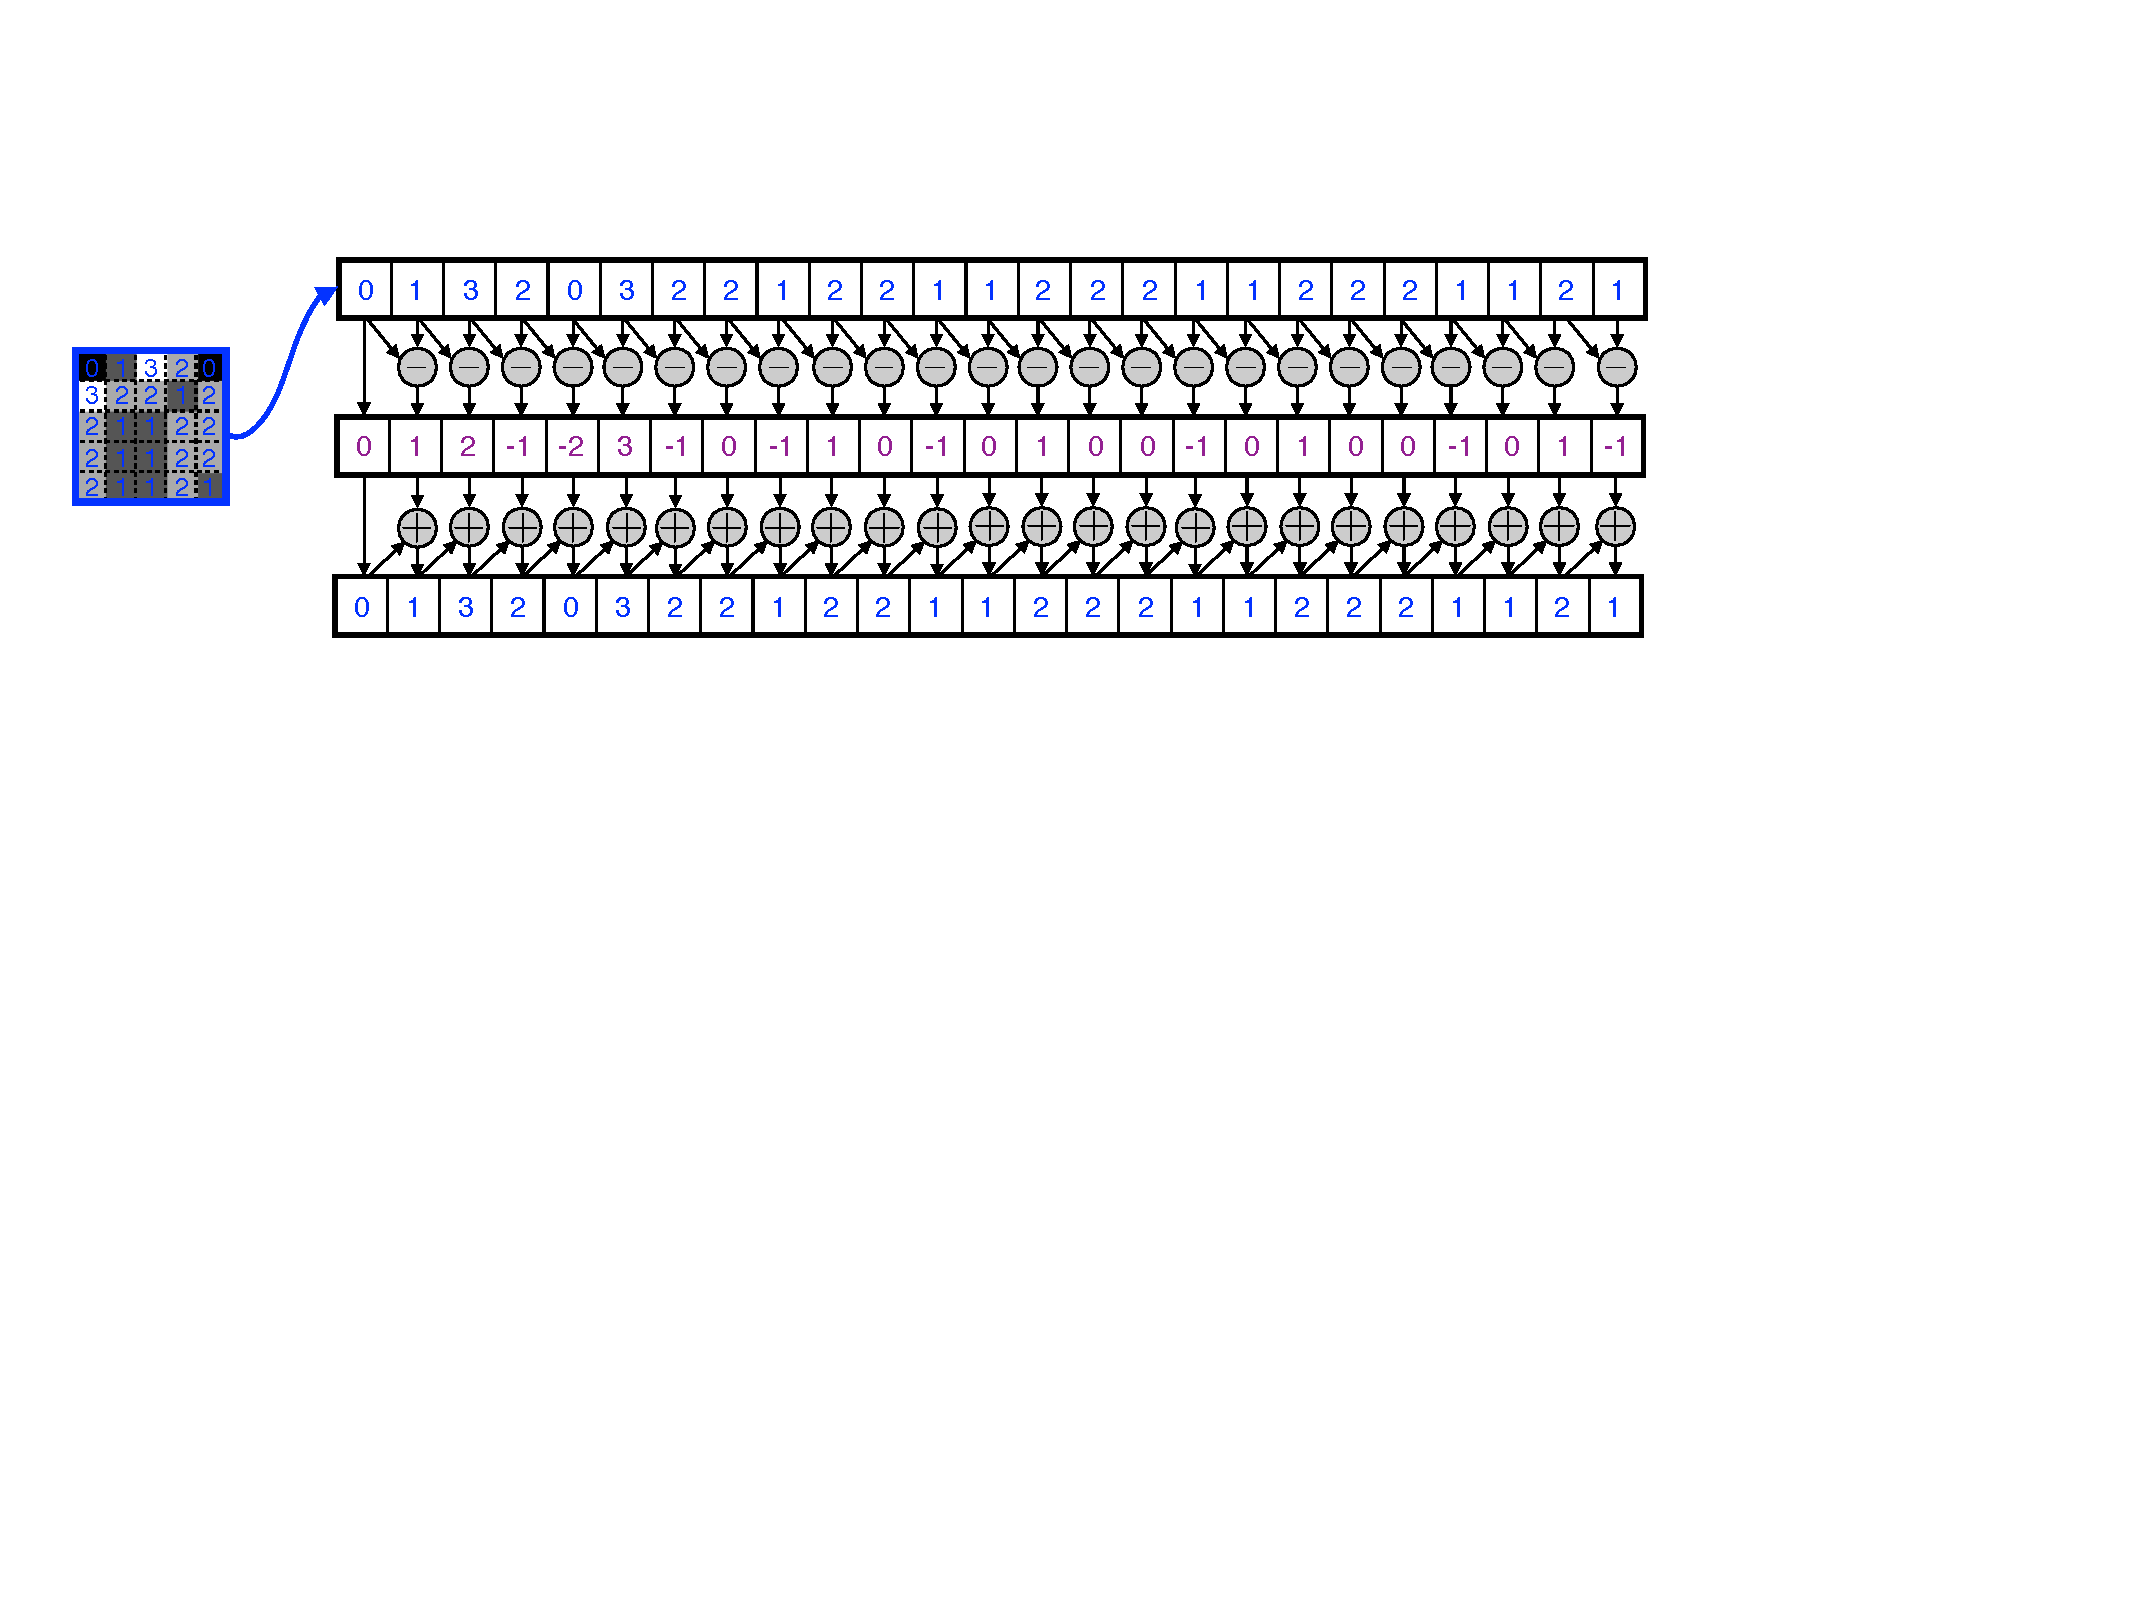
\includegraphics[width=\linewidth]{differences/differences}
}{fig-codage-differences}{Difference representation}

As the pixels can take values $\{\BL{0,1,2,3}\}$, the differences can take the values $\{\GR{-3, \ldots, 3}\}$. In particular, they may be negative (which does not pose any particular problem for defining a coding). The following figure compares the histograms of pixels and differences. We notice that the histogram of the differences is much more \guill{peaked} in the neighborhood of 0, which is logical, because many differences (corresponding to the homogeneous zones) are null or small. The entropy $\mathcal{H}_\Differ$ of the histogram of the differences (which can be modeled with a source $\Differ$) is therefore much lower than the entropy $\mathcal{H} \mot$ of the pixels.

The figure~\ref{fig-entropy-differences} shows a comparison of the histograms of pixel values and differences, calculated over the entire image (and not only on the initial 25 pixel subset).
%
It also shows the tree of an optimal prefix encoding (computed by the Huffman~\cite{Huffman52} algorithm) associated with the histogram of the differences.

\myfig{
\tabTrois{
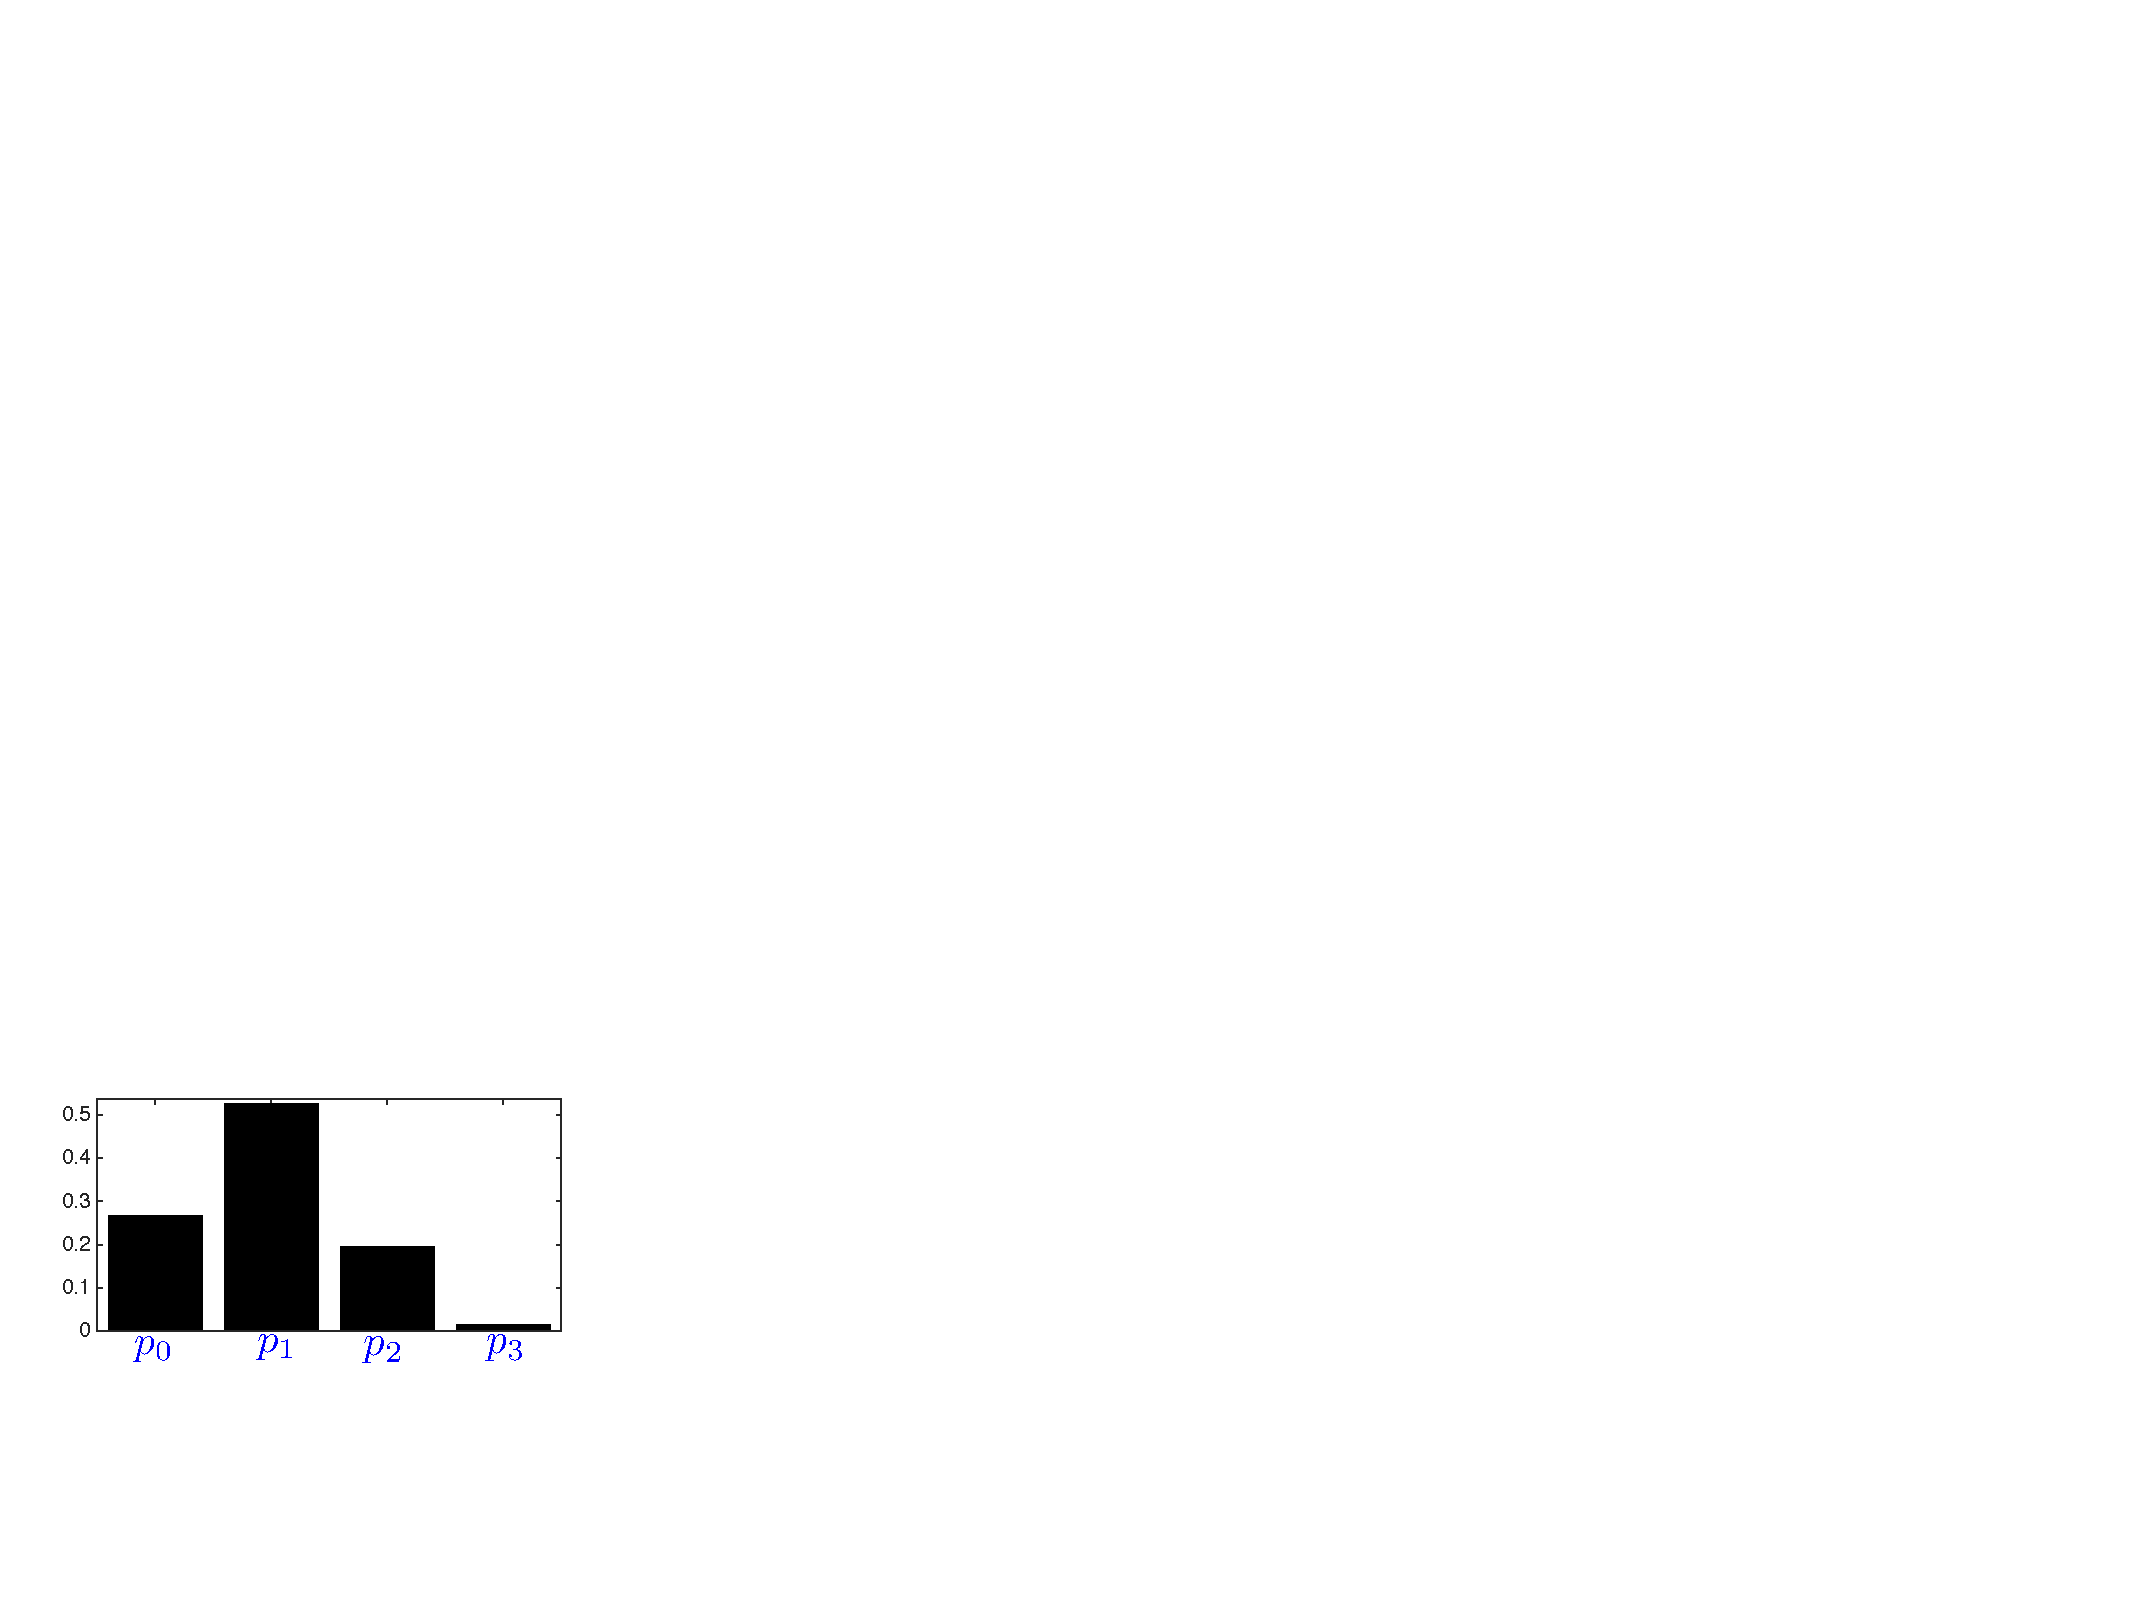
\includegraphics[width=.3\linewidth]{differences/histo-pix}&
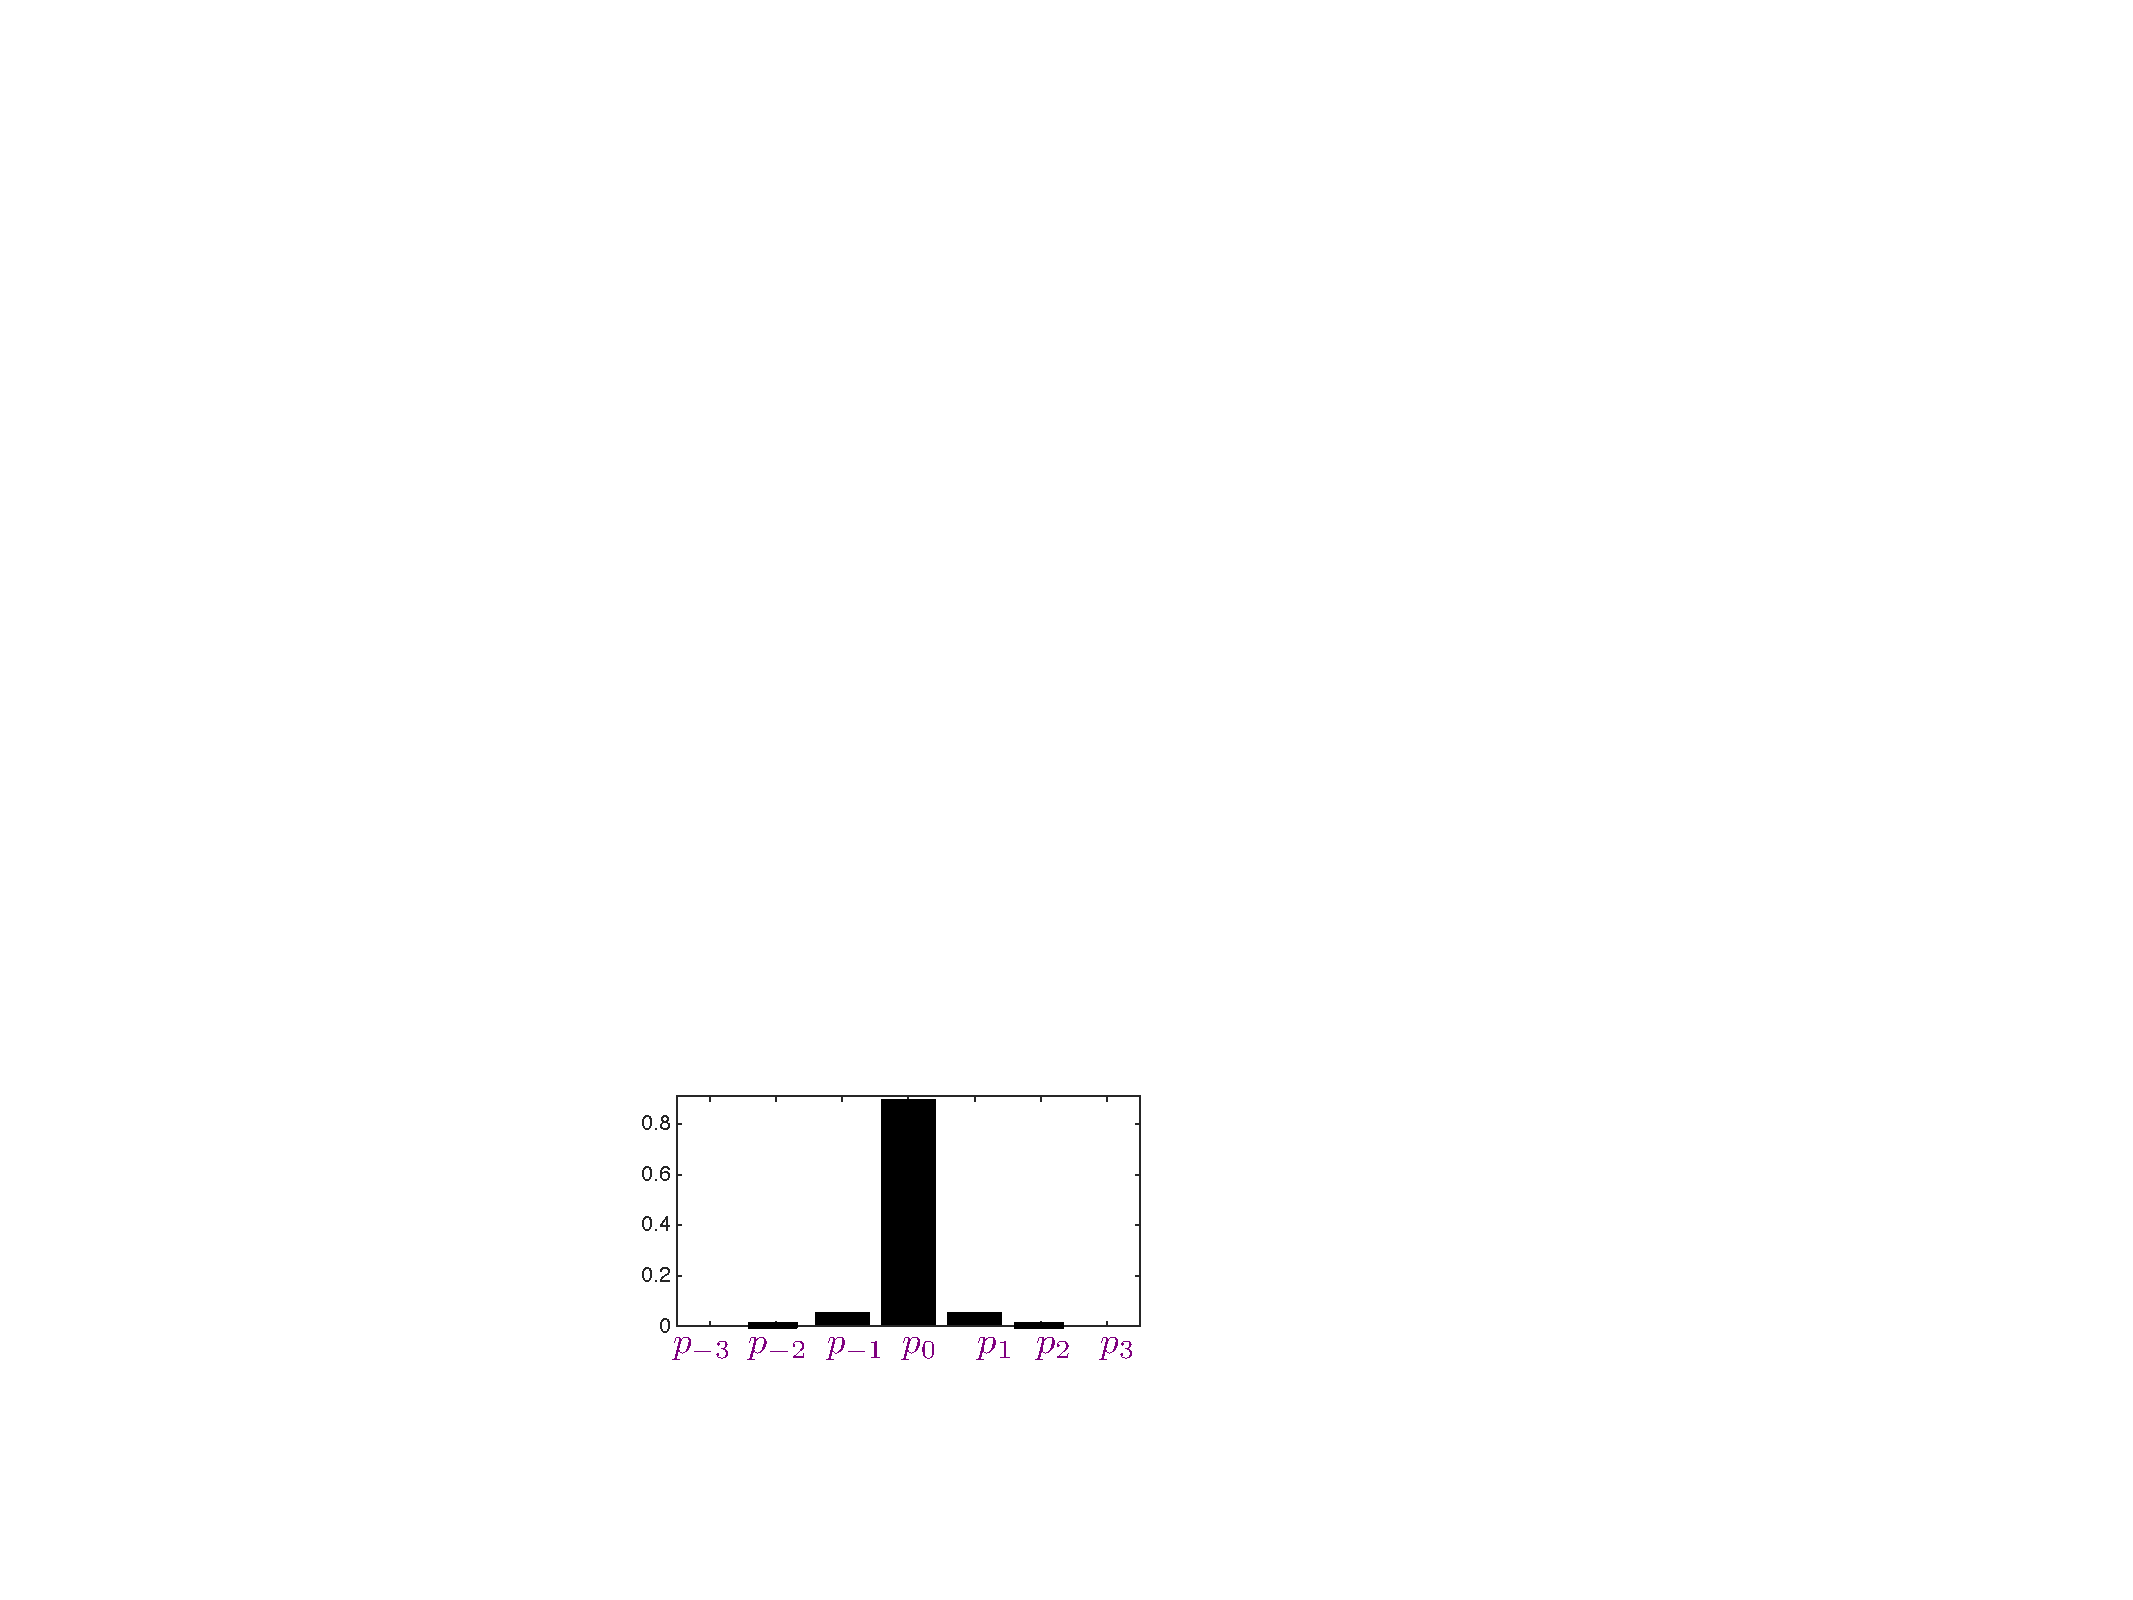
\includegraphics[width=.3\linewidth]{differences/histo-diff}&
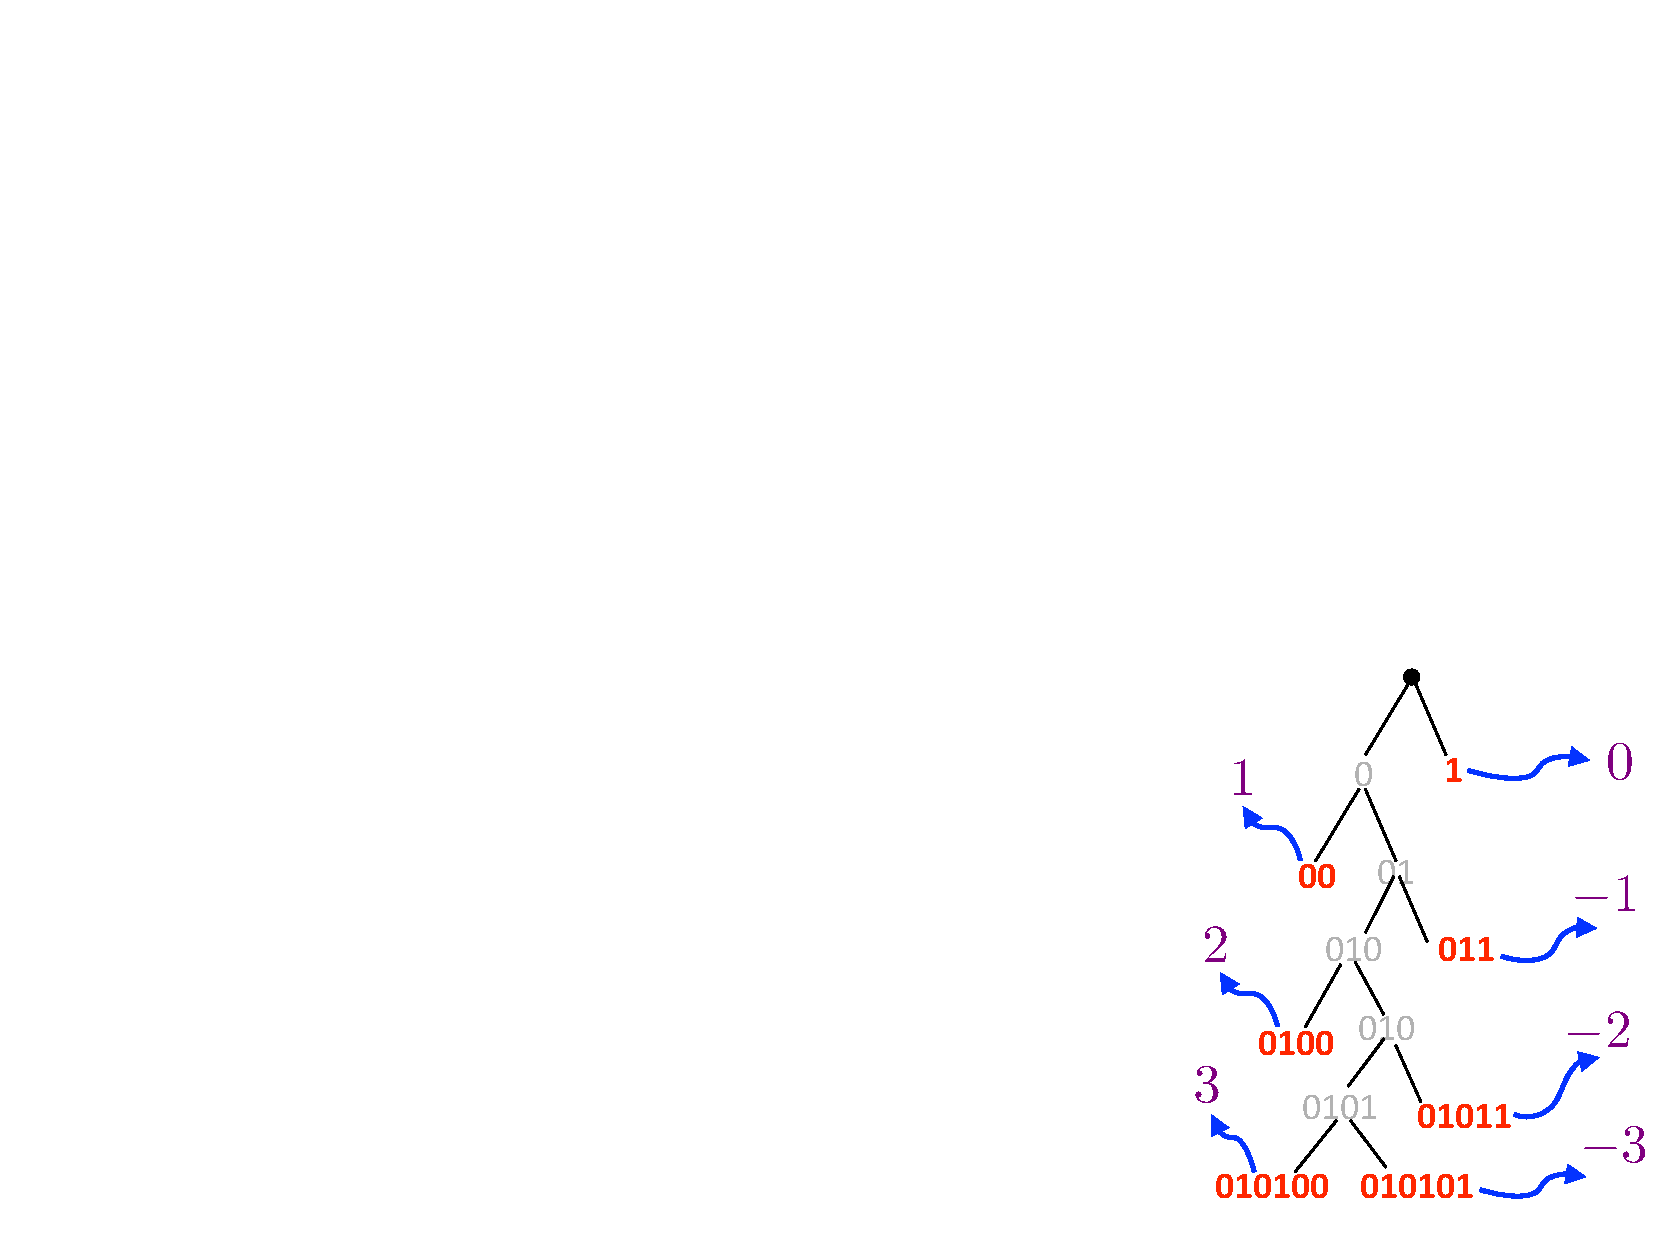
\includegraphics[width=.2\linewidth]{differences/arbre-difference}\\
$\Hh_{\mot} \approx 1.54, \LongMoy \approx 1.67 $ & $\Hh_{\Differ} \approx 0.61, \LongMoy \approx 1.16 $ & Coding Tree
}
}{fig-entropy-differences}{Comparison of histograms of pixel values and differences, and a code tree for these differences. }


This tree corresponds to the coding
$$
	\GR{-3} \mapsto \RE{010101},
	\GR{-2} \mapsto \RE{01011},
	\GR{-1} \mapsto \RE{011},
	\GR{0} \mapsto \RE{1},
	\GR{1} \mapsto \RE{00},
	\GR{2} \mapsto \RE{0100},
	\GR{3} \mapsto \RE{010100}.
$$
This encoding has an average length $\mathcal{L} \approx 1.16$ bits. This average number matches well to the entropy bound and is significantly smaller than the mean length associated with the pixel histogram (1.67 bits), which is itself smaller than the average length associated with a ($\log_2(4)=2 $ bits). If encode the entire image of $256 \times 256$ in gray level, we get the following gains, where 1kb=8 $\times$ 1024 bits is a \textit{kilo byte}.
\eq{
\begin{tabular}{c}
Uniform encoding \\
16.3 kb
\end{tabular}
\quad \longrightarrow \quad
\begin{tabular}{c}
Variable encoding \\
13.7 kb
\end{tabular}
\quad \longrightarrow \quad
\begin{tabular}{c}
Coding of differences \\
9.5 kb
\end{tabular}
}

The most efficient methods of image compression use more complex transformations, and exploit in a finer way the local regularity of the images. This is the case of the JPEG-2000\mylink{https://fr.wikipedia.org/wiki/JPEG_2000} compression method, which is considered to be the most efficient at the moment, using the wavelets\mylink{https://en.wikipedia.org/wiki/Ondelette}, see the book~\cite{mallat2009a-wav} for more details. There are many other cases where non-independence of symbols can be used to improve coding performance. An important example is the sequence of letters that compose a text.

%%%%%%%%%%%%%%%%%%%%%%%%%%%%%%%%%%%%%%%%%%%%%%%%%% %%%%%%%%%%%%%%%%%%%%%%%%%%%%%%%%
%%%%%%%%%%%%%%%%%%%%%%%%%%%%%%%%%%%%%%%%%%%%%%%%%% %%%%%%%%%%%%%%%%%%%%%%%%%%%%%%%%
%%%%%%%%%%%%%%%%%%%%%%%%%%%%%%%%%%%%%%%%%%%%%%%%%% %%%%%%%%%%%%%%%%%%%%%%%%%%%%%%%%
\section{Conclusion}

The mathematical theory initiated by Claude Shannon defines a framework necessary for the development of effective techniques for the acquisition, processing, storage and transmission of data in digital form. These techniques that revolutionized communications and computing during the second half of the 20th century, and enabled the growth of the Internet at the beginning of the 21st century. Without the revolutionary contributions of Shannon, you could not go on vacation with your entire library in your electronic reader, and all episodes of \textit{Game of Thrones} on your tablet!

For more details on the theory of information, one can have look at~\cite{CoverThomas}, for its use in signal and image processing, one can look at~\cite{mallat2009a-wav}.
The computer codes used to reproduce the figures in this article are available online at\mylink{https://github.com/gpeyre/2016-shannon-theory}, and other codes are available on the site \url{www.numerical-tours.com}~\cite{2011-peyre-cise}.

%%%%%%%%%%%%%%%%%%%%%%%%%%%%%%%%%%%%%%%%%%%%%%%%%% %%%%%%%%%%%%%%%%%%%%%%%%%%%%%%%%
%%%%%%%%%%%%%%%%%%%%%%%%%%%%%%%%%%%%%%%%%%%%%%%%%% %%%%%%%%%%%%%%%%%%%%%%%%%%%%%%%%
%%%%%%%%%%%%%%%%%%%%%%%%%%%%%%%%%%%%%%%%%%%%%%%%%% %%%%%%%%%%%%%%%%%%%%%%%%%%%%%%%%
\section*{Glossary}

\newcommand{\glossS}[1]{\item \textbf{#1}}

\begin{rs}
\glossS{Pixel}: location on the square grid of an image, sometimes used to refer to the associated value.
\glossS{Symbol}: element $\mot$ of a finite set, for example $\{0, \ldots, N-1\}$.
\glossS{Code}: $0$ and $1$ sequence used to encode a $\mot$ symbol.
\glossS{Coding}: set of correspondences between $\mot$ symbols and associated codes, for example $\BL{2} \mapsto \RE{10}$. Also refers to the action of replacing a sequence of symbols with a set of bits.
\glossS{Empirical distribution}: frequency $p_{\mot}$ of appearance of symbols $\mot$ in the sequence of symbols to be coded.
\glossS{Histogram}: graphical representation of the empirical distribution, which can also by extension designate this distribution.
\glossS{Source}: random variable $\Mot$ modeling the symbols, with the distribution $\mathbb{P}(\Mot=\mot)=p_{\mot}$.
\glossS{Entropy}: $\mathcal{H}_\mot$ is a positive number associated with the source $\Mot$ and depends on its probability distribution $(p_{\mot})_\mot$.
\glossS{Number of mean bits of a sequence:} $\mathcal{L}$ is associated with the encoding of a sequence of symbols.
\glossS{Number of source mean bits:} $\mathcal{L}_\mot$ is associated with the encoding of symbols generated by $\Mot$.
\end{rs}



%%%%%%%%%%%%%%%%%%%%%%%%%%%%%%%%%%%%%%%%%%%%%%%%%% %%%%%%%%%%%%%%%%%%%%%%%%%%%%%%%%
%%%%%%%%%%%%%%%%%%%%%%%%%%%%%%%%%%%%%%%%%%%%%%%%%% %%%%%%%%%%%%%%%%%%%%%%%%%%%%%%%%
%%%%%%%%%%%%%%%%%%%%%%%%%%%%%%%%%%%%%%%%%%%%%%%%%% %%%%%%%%%%%%%%%%%%%%%%%%%%%%%%%%
\section *{Acknowledgments}

I thank Marie-No�lle Peyr�, Gwenn Guichaoua, Fran�ois B\'eguin, G�rard Grancher, Aur�lien Djament and Fran�ois Sauvageot for their careful proofreading of a French version of this text.

The image of the flower is due to Maitine Bergounioux. The image of Shannon used for the logo of the article is due to the telehistoriska user of the flickr site (under license CC-BY-NC-2.0).




% !TEX root = ../IntroImaging-FR.tex

\chapter{Le traitement d'images}
\label{chap-images}

\newcommand{\FootLink}[1]{\footnote{\url{#1}}}
\newcommand{\myparagraph}[1]{\vspace{2mm}\noindent\textbf{#1}}
\newcommand{\lien}[2]{#2}

%\newcommand{\bs}{\_}

\newcommand{\BetweenImageSpace}{\hspace{3mm}}

\newcommand{\image}[1]{\includegraphics[width=0.32\linewidth]{#1}}
\newcommand{\imageM}[1]{\includegraphics[width=0.4\linewidth]{#1}}
\newcommand{\imageL}[1]{\includegraphics[width=0.6\linewidth]{#1}}
\newcommand{\imageQuad}[8]{
\begin{tabular}{@{}c@{\BetweenImageSpace{}}c@{}}
\image{#1} & \image{#2}\\
#5 & #6 \\
\image{#3} & \image{#4}\\
#5 & #6 
\end{tabular}
}
\newcommand{\imageTri}[6]{
\begin{tabular}{@{}c@{\BetweenImageSpace{}}c@{\BetweenImageSpace{}}c@{}}
\image{#1} & \image{#2} & \image{#3}\\
#4 & #5 & #6 \\
\end{tabular}
}
\newcommand{\imageDuo}[4]{
\begin{tabular}{@{}c@{\BetweenImageSpace{}}c@{}}
\image{#1} & \image{#2} \\
#3 & #4  \\
\end{tabular}
}

\newcommand{\myfigure}[3]{
    \begin{figure}[ht]
    \begin{center}
        #1                          % usual include graphics
    \end{center}
    \vspace{-4mm}
        \caption{\textit{#2}}       % caption
    \label{#3}          % label
    \end{figure}
}



Les appareils num�riques photographient de mani�re tr�s pr�cise le monde qui nous entoure. L'utilisateur souhaite pouvoir stocker avec un encombrement minimal ses photos sur son disque dur. Il souhaite �galement pouvoir les retoucher afin d'am�liorer leur qualit�. Cet article pr�sente les outils math�matiques et informatiques qui permettent d'effectuer ces diff�rentes t�ches. Il reprend en partie le contenu de l'article publi� sur le site web \textit{Images des math�matiques}\FootLink{http://images.math.cnrs.fr/Le-traitement-numerique-des-images.html}.


%%%%%%%%%%%%%%%%%%%%%%%%%%%%%%%%%%%%%%%%%%%%%%%%%%%%%%%%%%%%%%
%%%%%%%%%%%%%%%%%%%%%%%%%%%%%%%%%%%%%%%%%%%%%%%%%%%%%%%%%%%%%%
%%%%%%%%%%%%%%%%%%%%%%%%%%%%%%%%%%%%%%%%%%%%%%%%%%%%%%%%%%%%%%
\section{Les pixels d'une image}

Une \lien{http://fr.wikipedia.org/wiki/Image\bs{}num\%C3\%A9rique}{image num�rique}
en niveaux de gris est un tableau de valeurs. Chaque
case de ce tableau, qui stocke une valeur, se nomme un 
\lien{http://fr.wikipedia.org/wiki/Pixel}{pixel}. 
En notant \(n\) le nombre de lignes et \(p\) le nombre de colonnes de l'image, 
on manipule ainsi un tableau de \(n \times p\) pixels. La figure \ref{fig-section1-original-zoom}, gauche, montre une visualisation d'un tableau carr� avec  \(n=p=240\), ce qui repr�sente  \(240\times 240\)=57600 pixels. Les
\lien{http://fr.wikipedia.org/wiki/Appareil\bs{}photographique\bs{}num\%C3\%A9rique}{appareils photos num�riques} 
peuvent enregistrer des images beaucoup plus grandes,
avec plusieurs 
\lien{http://en.wikipedia.org/wiki/Gigapixel\bs{}image}{millions de pixels}.

Les valeurs des pixels sont enregistr�es dans 
\lien{http://fr.wikipedia.org/wiki/Ordinateur}{l'ordinateur} ou
\lien{http://fr.wikipedia.org/wiki/Appareil\bs{}photographique\bs{}num\%C3\%A9rique}{l'appareil photo num�rique} 
sous forme de 
\lien{http://fr.wikipedia.org/wiki/Entier\bs{}relatif}{nombres entiers} entre 0 et $255=2^8-1$, 
ce qui fait 256 valeurs possibles pour chaque pixel. La valeur 0 correspond au noir, et la valeur 255 correspond au blanc. Les valeurs interm�diaires correspondent � des 
\lien{http://fr.wikipedia.org/wiki/Niveau\bs{}de\bs{}gris}{niveaux de gris}
allant du noir au blanc. La figure \ref{fig-section1-original-zoom} montre un sous-tableau de \(6 \times 6\) pixels extrait de l'image pr�c�dente. On peut voir � la fois les valeurs qui composent le tableau et les niveaux de gris qui permettent d'afficher l'image � l'�cran.
  
\myfigure{
\imageL{section1-original-zoom}
}{Sous image de taille $5 \times 5$}{fig-section1-original-zoom}


%%%%%%%%%%%%%%%%%%%%%%%%%%%%%%%%%%%%%%%%%%%%%%%%%%%%%%%%%%%%%%
%%%%%%%%%%%%%%%%%%%%%%%%%%%%%%%%%%%%%%%%%%%%%%%%%%%%%%%%%%%%%%
%%%%%%%%%%%%%%%%%%%%%%%%%%%%%%%%%%%%%%%%%%%%%%%%%%%%%%%%%%%%%%
\section{Stocker une image}

%%%%%%%%%%%%%%%%%%%%%%%%%%%%%%%%%%%%%%%%%%%%%%%%%%%%%%%%%%%%%%
\subsection{\'Ecriture binaire}

Stocker de grandes images sur le 
\lien{http://fr.wikipedia.org/wiki/Disque\bs{}dur}{disque dur}
d'un ordinateur prend
beaucoup de place. Les nombres entiers sont stock�s 
en 
\lien{http://fr.wikipedia.org/wiki/Syst\%C3\%A8me\bs{}binaire}{�criture binaire}, 
c'est-�-dire sous la forme d'une succession
de 0 et de 1. Chaque 0 et chaque 1 se stocke sur une unit� �l�mentaire
de stockage, appel�e 
\lien{http://fr.wikipedia.org/wiki/Bit}{bit}.
Pour obtenir l'�criture binaire d'un pixel ayant comme valeur 179, 
il faut d�composer cette valeur comme somme de puissances de deux. 
On obtient ainsi
\[ 179=2^7+2^5+2^4+2+1, \]
o� l'on a pris soin d'ordonner les puissances de deux par ordre
d�croissant. Afin de faire mieux appara�tre l'�criture binaire, 
on ajoute "\(1 \times\)" devant chaque puissance qui appara�t dans l'�criture, 
et "\(0\times\)" devant les puissances qui n'apparaissent pas
\[ 179=1 \times 2^7 + 0 \times 2^6 + 1 \times 2^5 + 1 \times 2^4 + 
  0 \times 2^3 + 0 \times 2^2 + 1 \times 2^1 + 1 \times 2^0. \]
Avec une telle �criture, la valeur de chaque pixel, qui est un nombre entre 0 et 255, n�cessite 
\( \log_2(256) = 8 \text{ bits}. \)
% La fonction \(\log_2\) est le logarithme en base 2, et ce calcul exprime
% le fait que  \( 256=2^8 \)
%  = 2 \times 2 \times 2 \times 2 \times 2 \times 2 \times 2 \times 2.  \]
L'�criture binaire de la valeur 179 du pixel est ainsi \((1,0,1,1,0,0,1,1)\).
% o� chaque 1 et chaque 0 correspond au facteur multiplicatif qui appara�t devant chaque puissance.
On peut �crire toute valeur entre 0 et 255 de cet mani�re,
ce qui n�cessite d'utilisation de 8 bits. Il y a en effet 
256 valeurs possibles, et \(256=2^8\). Pour stocker l'image compl�te, on a donc besoin de
\( n \times p \times 8 \text{ bits}. \)
Pour l'image montr�e aux figure pr�c�dentes, on a ainsi besoin de 
\[ 256 \times 256 \times 8 = 524288 \text{ bits}. \]
On utilise le plus souvent 
\lien{http://fr.wikipedia.org/wiki/Octet}{l'octet} (8 bits) comme unit�,
de sorte que cette image n�cessite 57,6ko (kilo octets).


%%%%%%%%%%%%%%%%%%%%%%%%%%%%%%%%%%%%%%%%%%%%%%%%%%%%%%%%%%%%%%
\subsection{Sous-�chantilloner une image}


% on peut r�duire sa
% \lien{http://fr.wikipedia.org/wiki/R\%C3\%A9solution\bs{}(imagerie\bs{}num\%C3\%A9rique)}{r�solution},  c'est-�-dire

\myfigure{
\imageTri
%{section2-subsample-2}
{section2-subsample-4}
{section2-subsample-8}
{section2-subsample-16}
%{Une ligne/colonne sur 2}
{Une ligne/colonne sur 4}
{Une ligne/colonne sur 8}
{Une ligne/colonne sur 16}
}{Sous-�chantillonnage d'une image}{fig-section2-subsample}

Afin de r�duire la place de stockage d'une image on peut diminuer le nombre de pixels.
La fa�on la plus simple d'effectuer cette r�duction consiste � supprimer des lignes et des colonnes dans l'image de d�part. La figure \ref{fig-section2-subsample}, en haut � gauche, montre ce que l'on obtient si l'on retient une ligne sur 4 et une colonne sur 4. On a ainsi divis� par \(4 \times 4 = 16\) le nombre de pixels de l'image,
et donc �galement divis� par 16 le nombre de bits n�cessaire pour stocker l'image sur 
un disque dur. Sur la figure \ref{fig-section2-subsample}, on peut voir les r�sultats obtenus en enlevant de plus en
plus de lignes et de colonnes. Bien entendu, la qualit� de l'image se
d�grade vite.



%%%%%%%%%%%%%%%%%%%%%%%%%%%%%%%%%%%%%%%%%%%%%%%%%%%%%%%%%%%%%%
\subsection{Quantifier une image}

Une autre fa�on de r�duire la place m�moire n�cessaire pour le stockage
consiste � utiliser moins de nombres entiers pour chaque valeur. On peut par exemple utiliser uniquement des nombres entiers entre 0 et 3, ce qui donnera une image avec uniquement 4 niveaux de gris.  On peut effectuer une conversion de l'image d'origine vers une image avec 4 niveaux de valeurs en effectuant les remplacements:
\begin{rs}
\item les valeurs dans \(0,1,\ldots,63\) sont remplac�es par la valeur 0 (noir), 
\item les valeurs dans \(64,1,\ldots,127\) sont remplac�es par la valeur 1 (gris clair), 
\item les valeurs dans \(128,1,\ldots,191\) sont remplac�es par la valeur 2 (gris fonc�), 
\item les valeurs dans \(192,\ldots,255\) sont remplac�es par la valeur 3 (blanc).
\end{rs}
Une telle op�ration se nomme \lien{http://fr.wikipedia.org/wiki/Quantification\bs{}(signal)}{quantification}. La \ref{fig-section3-quantize}, au centre, suivante montre l'image r�sultante avec 4 niveaux de couleurs.

Nous avons d�j� vu que l'on pouvait repr�senter toute valeur entre 0 et
255 � l'aide de 8 bits en utilisant l'�criture binaire. De fa�on similaire, 
on v�rifie que toute valeur entre 0 et 3 peut se repr�senter � l'aide de 2 bits. 
On obtient ainsi une r�duction d'un facteur 8/2=4 de la place 
\lien{http://fr.wikipedia.org/wiki/M\%C3\%A9moire\bs{}(informatique)}{m�moire} 
n�cessaire 
pour le stockage de l'image sur un disque dur. La figure \ref{fig-section3-quantize} montre les r�sultats obtenus en utilisant de moins en moins de niveaux de gris.

\myfigure{
\imageDuo
%{section3-quantize-2}
%{section3-quantize-3}
{section3-quantize-4}
{section3-quantize-16}
%{16 niveaux de gris}
%{3 niveaux de gris}
{4 niveaux de gris}
{16 niveaux de gris}
}{Quantification d'une image
}{fig-section3-quantize}
 
Tout comme pour la r�duction du nombre de pixels, la r�duction du nombre
de niveaux de gris influe beaucoup sur la qualit� de l'image. 
Afin de r�duire au maximum la taille d'une image sans modifier sa qualit�,
on utilise des m�thodes plus complexes de 
\lien{http://fr.wikipedia.org/wiki/Compression\bs{}d\%27image}{compression d'image}. 
% \ArticleAPMEP{La vignette Klein de ce num�ro d�taille une m�thode qui exploite la d�composition en valeurs singuli�res des matrices.}


La m�thode  la plus efficace s'appelle
\lien{http://fr.wikipedia.org/wiki/Jpeg\bs{}2000}{JPEG-2000}. 
Elle utilise la th�orie des 
\lien{http://fr.wikipedia.org/wiki/Ondelettes}{ondelettes}.
Pour en savoir plus � ce sujet, vous pouvez consulter l'article d'Erwan Le Pennec sur le site web \textit{Images des math�matiques}\FootLink{http://images.math.cnrs.fr/Compression-d-image.html}. 





%%%%%%%%%%%%%%%%%%%%%%%%%%%%%%%%%%%%%%%%%%%%%%%%%%%%%%%%%%%%%%
%%%%%%%%%%%%%%%%%%%%%%%%%%%%%%%%%%%%%%%%%%%%%%%%%%%%%%%%%%%%%%
%%%%%%%%%%%%%%%%%%%%%%%%%%%%%%%%%%%%%%%%%%%%%%%%%%%%%%%%%%%%%%
\section{Enlever le bruit}

%%%%%%%%%%%%%%%%%%%%%%%%%%%%%%%%%%%%%%%%%%%%%%%%%%%%%%%%%%%%%%
\subsection{Moyenne locale}

Les images sont parfois de mauvaise qualit�. Un exemple typique de d�faut
est le 
\lien{http://fr.wikipedia.org/wiki/Bruit\bs{}num\%C3\%A9rique}{\guill{bruit}}
qui apparait quand une photo est 
\lien{http://fr.wikipedia.org/wiki/Exposition\bs{}(photographie)}{sous-expos�e}, 
c'est-�-dire
qu'il n'y a pas assez de luminosit�. Ce bruit se manifeste par de petites
fluctuations 
\lien{http://fr.wikipedia.org/wiki/Suite\bs{}al\%C3\%A9atoire}{al�atoires}
des niveaux de gris. La figure \ref{fig-section5-moyenne}, � gauche, montre
une image bruit�e. 



\myfigure{
\imageM{section5-moyenne-numbers}
}{Voisinage de pixels.
}{fig-section5-moyenne-numbers}

Afin d'enlever le bruit dans les images, il convient de faire subir une
modification aux valeurs de pixels. 
L'op�ration la plus simple consiste � remplacer la valeur 
\(a\) de chaque pixel par la 
\lien{http://fr.wikipedia.org/wiki/Moyenne}{moyenne}
de  \(a\) et des 8 valeurs \(b,c,d,e,f,g,h,i\) des 8 pixels qui entourent $a$ . La figure \ref{fig-section5-moyenne-numbers} montre un exemple de voisinage de 9 pixels. On obtient ainsi une image modifi�e en rempla�ant a par
\[ \frac{a+b+c+d+e+f+g+h+i}{9} \]
puisque l'on fait la moyenne de 9 valeurs.
Dans notre exemple, cette moyenne vaut
\[ \frac{190+192+79+54+47+153+203+189+166}{9} \approx 141. \]
En effectuant cette op�ration pour chaque pixel, on supprime une partie 
du bruit, car ce bruit est constitu� de fluctuations al�atoires, qui sont
diminu�es par un calcul de moyennes. La figure \ref{fig-section5-moyenne}, en haut � gauche, montre l'effet d'un tel calcul. Tout le bruit n'a pas �t� enlev� par cette op�ration. Afin d'enlever plus
de bruit, on peut moyenner plus de valeurs autour de chaque pixel.
La figure \ref{fig-section5-moyenne} montre le r�sultat obtenu en moyennant de plus en plus
de valeurs. 


\myfigure{
\imageTri
{section5-moyenne-1}
{section5-moyenne-2}
{section5-moyenne-3}
%{section5-moyenne-4}
{Moyenne sur 9 pixels}
{Moyenne sur 25 pixels}
{Moyenne sur 49 pixels}
%{Moyenne sur 81 pixels}
}{Moyenne de plus en plus forte
}{fig-section5-moyenne}

Le moyennage des pixels est tr�s efficace pour enlever le bruit dans les
images, malheureusement il d�truit �galement une grande partie de
l'information de l'image. On peut en effet s'aper\-ce\-voir que les images
obtenues par moyennage sont 
\lien{http://fr.wikipedia.org/wiki/Flou,\bs{}nettet\%C3\%A9\bs{}et\bs{}contraste}{floues}. 
Ceci est en particulier visible pr�s
des contours, qui ne sont pas nets.

%%%%%%%%%%%%%%%%%%%%%%%%%%%%%%%%%%%%%%%%%%%%%%%%%%%%%%%%%%%%%%
\subsection{M�diane locale}

Afin de r�duire ce flou, on remplace la moyenne par la m�diane. Dans l'exemple du voisinage de 9 pixels utilis� � la section pr�c�dente, les 9 valeurs class�es sont :
\[ 47,54,79,153,166,189,190,192,203. \]
La m�diane de ces neuf valeurs est 166.  Afin d'enlever plus de bruit, il suffit de calculer la m�diane sur un nombre plus grand de pixels voisins, comme montr� � la figure \ref{fig-section6-mediane}.
On constate que cette m�thode est plus performante que le calcul de
moyennes, car les images r�sultantes sont moins floues. Cependant, tout comme 
avec le calcul de moyennes, si l'on prend des voisinages trop grands, on perd
aussi de l'information de l'image, en particulier les bords des objets sont d�grad�s.


\if 0
Afin de r�duire ce flou, il faut remplacer le moyennage par une op�ration
un peu plus complexe, que l'on nomme 
\lien{http://fr.wikipedia.org/wiki/M\%C3\%A9diane}{mediane}. Etant donn� la valeur \(a\) d'un pixel, et les valeurs
\(b,c,d,e,f,g,h,i\), on commence par les classer 
par 
\lien{http://fr.wikipedia.org/wiki/Ordre\bs{}croissant}{ordre croissant}.
Dans l'exemple du voisinage de 9 pixels utilis� � la section pr�c�dente, 
on obtient les 9 valeurs class�es
\[ 47,54,79,153,166,189,190,192,203. \]
La m�diane des neuf valeurs \(a,b,c,d,e,f,g,h,i\)
est la \(5^\text{e}\) valeur de ce classement (c'est-�-dire la 
valeur centrale de ce classement).

Dans notre cas, la m�diane est donc 166. Notez que ce nombre est en g�n�ral diff�rent de la moyenne.

\fi


\myfigure{
\imageTri
{section6-mediane-1}
{section6-mediane-2}
{section6-mediane-3}
%{section6-mediane-4}
{M�diane sur 9 pixels}
{M�diane sur 25 pixels}
{M�diane sur 49 pixels}
%{M�diane sur 81 pixels}
}{Filtrage m�dian de plus plus en plus fort.
}{fig-section6-mediane}




%%%%%%%%%%%%%%%%%%%%%%%%%%%%%%%%%%%%%%%%%%%%%%%%%%%%%%%%%%%%%%
%%%%%%%%%%%%%%%%%%%%%%%%%%%%%%%%%%%%%%%%%%%%%%%%%%%%%%%%%%%%%%
%%%%%%%%%%%%%%%%%%%%%%%%%%%%%%%%%%%%%%%%%%%%%%%%%%%%%%%%%%%%%%
\section{D�tecter les bords des objets}

Afin de localiser des objets dans les images, il est n�cessaire de
d�tecter les 
\lien{http://fr.wikipedia.org/wiki/D\%C3\%A9tection\bs{}de\bs{}contours}{bords}
de ces objets. Ces bords correspondent � des 
zones de l'image o� les valeurs des pixels changent rapidement. C'est le
cas par exemple lorsque l'on passe de la coque du bateau (qui est sombre,
donc avec des valeurs petites) � la mer (qui est claire, donc avec des
valeurs grandes).

Afin de savoir si un pixel avec une valeur \(a\) est le long d'un bord d'un objet, on prend en compte les valeurs \(b,c,d,e\) de ses quatre voisins qui ont un c�t� commun avec lui (figure \ref{fig-section7-contours-numbers}).  Ceci permet de d�tecter aussi pr�cis�ment que possible les bords des objets. 

\if 0
(deux horizontalement et deux verticalement), qui sont dispos�s par rapport � \(a\) comme illustr� � la figure \ref{fig-section7-contours-numbers}. Notons que l'on utilise ici seulement les 4 voisins qui ont un cot� commun avec le pixel consid�r�, ce qui est diff�rent du calcul de moyennes et de m�dianes o� l'on utilisait 8 voisins. Ceci est important afin de d�tecter aussi pr�cis�ment que possible les bords des objets.
\fi 


\myfigure{
\imageM{section7-contours-numbers}
}{Exemple d'un voisinage de 5 pixels.
}{fig-section7-contours-numbers}


On calcule une valeur \(\ell\) suivant la formule
\[ \ell = \sqrt{ (b-d)^2 + (c-e)^2 }.  \]
Dans notre exemple, on obtient donc
\[ \ell= \sqrt{�(192 - 153)^2 + (189 - 54)^2 } = \sqrt{19746} \approx 141. \]
On peut remarquer que si \(\ell=0\), alors on a \(b=c\)
et \(d=e\). Au contraire, si 
\(\ell\) est grand, ceci signifie que les pixels voisins ont des valeurs tr�s
diff�rentes, le pixel consid�r� est donc probablement sur le bord d'un objet. 

La figure \ref{fig-section7-contours} montre une image dont la valeur des pixels est $\min(\ell,255)$. 
Il est n�cessaire de prendre le minium avec 255, car la valeur de $\ell$ peut d�passer la valeur maximale affichable (255, qui correspond au blanc). On a ainsi affich� ces valeurs avec du noir quand \(\ell=0\),  du blanc quand \(\ell\) est grand, et on a utilis� des niveaux de gris pour les valeurs interm�diaires. On peut voir que dans l'image de droite, les contours des objets ressortent en blanc, car ils correspondent aux grandes valeurs de \(\ell\).

\myfigure{
\imageDuo
{section7-image}
{section7-contours}
{Image d'origine}
{Carte de contours $\ell$}
}{D�tection des bords.
}{fig-section7-contours}

%%%%%%%%%%%%%%%%%%%%%%%%%%%%%%%%%%%%%%%%%%%%%%%%%%%%%%%%%%%%%%
%%%%%%%%%%%%%%%%%%%%%%%%%%%%%%%%%%%%%%%%%%%%%%%%%%%%%%%%%%%%%%
%%%%%%%%%%%%%%%%%%%%%%%%%%%%%%%%%%%%%%%%%%%%%%%%%%%%%%%%%%%%%%
\section{Les images couleurs}


%%%%%%%%%%%%%%%%%%%%%%%%%%%%%%%%%%%%%%%%%%%%%%%%%%%%%%%%%%%%%%
\subsection{Espace RVB}

Une 
\lien{http://fr.wikipedia.org/wiki/Couleur}{image couleur}
est en r�alit� compos�e de trois images ind�pendantes,
afin de repr�senter le
\lien{http://fr.wikipedia.org/wiki/Rouge\bs{}vert\bs{}bleu}{rouge, le vert, et le bleu}. 
Chacune de ces trois
images s'appelle un 
\lien{http://fr.wikipedia.org/wiki/Codage\bs{}informatique\bs{}des\bs{}couleurs}{canal}.
Cette repr�sentation en rouge, vert et bleu mime le fonctionnement du
syst�me visuel humain.
La figure \ref{fig-canaux-coul} montre les trois canaux constitutifs de l'image montr�e sur la gauche de la figure \ref{fig-luminance}.

\myfigure{
\imageDuo
{section8-image}
{section8-luminance}
{Image d'origine}
{Luminance}
}{Image couleur.
}{fig-luminance}


Chaque pixel de l'image couleur contient ainsi trois nombres \( (r,v,b) \),
chacun �tant un nombre entier entre 0 et 255.
Si le pixel est �gal � \((r,v,b)=(255,0,0)\), il ne contient que de l'information
rouge, et est affich� comme du rouge. 
De fa�on similaire, les pixels valant \((0,255,0)\) et \((0,0,255)\) sont
respectivement affich�s vert et bleu.


\myfigure{
\imageTri
{section8-rouge}
{section8-vert}
{section8-bleu}
{Canal rouge}
{Canal vert}
{Canal bleu}
}{Canaux couleurs
}{fig-canaux-coul}


On peut afficher � l'�cran une image couleur �
partir de ses trois canaux \((r,v,b)\) en utilisant les r�gles de la 
\lien{http://fr.wikipedia.org/wiki/Synth\%C3\%A8se\bs{}additive}{synth�se additive des couleurs}. Ces r�gles correspondent � la fa�on dont les rayons lumineux se combinent, d'o� le qualificatif \guill{additif}.  
La figure \ref{fig-section8-synthese}, gauche, montre les r�gles de composition
cette synth�se additive des couleurs. 
Par exemple un pixel avec les valeurs
\((r,v,b)=(255,0,255)\) est un m�lange de rouge et de vert, il est donc
affich� comme du jaune.


\myfigure{
\imageDuo
{section8-synthese-additive}
{section8-synthese-soustractive}
{Synth�se additive}
{Synth�se soustractive}
}{Synth�se des couleurs
}{fig-section8-synthese}


%%%%%%%%%%%%%%%%%%%%%%%%%%%%%%%%%%%%%%%%%%%%%%%%%%%%%%%%%%%%%%
\subsection{Espace CMJ}

Une autre repr�sentation courante pour les images couleurs utilise
comme couleurs de base le cyan, le magenta et le jaune. On calcule 
les trois nombres \((c,m,j)\) correspondant � chacun de ces trois canaux � 
partir des canaux rouge, vert et bleu \((r,v,b)\) comme suit
\[ c=255-r, \quad m=255-v, \quad j=255-b. \]
Par exemple, un pixel de bleu pur 
\((r,v,b)=(0,0,255)\) va devenir 
\( (c,m,j)=(255,255,0) \). La figure suivante montre les trois canaux
\((c,m,j)\) d'une image couleur.

\myfigure{
\imageTri
{section8-cyan}
{section8-magenta}
{section8-jaune}
{Canal cyan}
{Canal magenta}
{Canal jaune}
}{Canaux CMJ
}{fig-canaux-cmj}


Afin d'afficher une image couleur � l'�cran � partir des trois canaux \((c,m,j)\), on doit utiliser la synth�se soustractive des couleurs. La figure \ref{fig-section8-synthese}, droite, montre les r�gles de composition cette synth�se soustractive. Elle correspondent en peinture � l'absorption de la lumi�re par les pigments color�s, d'o� le qualificatif \guill{soustractif}. Le cyan, le magenta et le jaune sont appel�s couleurs primaires.

On peut donc stocker sur un disque dur une image couleur en stockant les
trois canaux, correspondant aux valeurs \((r,g,b)\) ou \((c,m,j)\). 
On peut modifier les images couleur tout comme les images en niveaux de
gris. La fa�on la plus simple de proc�der consiste � appliquer la modification
� chacun des canaux.


%%%%%%%%%%%%%%%%%%%%%%%%%%%%%%%%%%%%%%%%%%%%%%%%%%%%%%%%%%%%%%
%%%%%%%%%%%%%%%%%%%%%%%%%%%%%%%%%%%%%%%%%%%%%%%%%%%%%%%%%%%%%%
%%%%%%%%%%%%%%%%%%%%%%%%%%%%%%%%%%%%%%%%%%%%%%%%%%%%%%%%%%%%%%
\section{Changer le contraste d'une image}

%%%%%%%%%%%%%%%%%%%%%%%%%%%%%%%%%%%%%%%%%%%%%%%%%%%%%%%%%%%%%%
\subsection{Luminance}

On peut calculer une image en niveaux de gris � partir d'une image couleur
en moyennant les trois canaux. On calcule donc, pour chaque pixel, une valeur 
\[ a = \frac{r+v+b}{3} \]
qui s'appelle la 
\lien{http://fr.wikipedia.org/wiki/Luminance}{luminance} 
de la couleur. La figure \ref{fig-luminance}  montre le passage d'une image couleur � une image de luminance en
niveaux de gris. 


%%%%%%%%%%%%%%%%%%%%%%%%%%%%%%%%%%%%%%%%%%%%%%%%%%%%%%%%%%%%%%
\subsection{Manipulations du contraste en niveaux de gris}

Il est possible de faire subir diff�rentes modifications � l'image afin de
changer son 
\lien{http://fr.wikipedia.org/wiki/Contraste}{contraste}. On consid�re ici une image en niveaux de gris.
Un manipulation simple consiste � remplacer chaque valeur \(a\) d'un pixel d'une image par \(255-a\) ce qui correspond � l'intensit� de gris oppos�e. Le blanc devient noir et vice-et-versa, ce qui donne un effet similaire � celui
des 
\lien{http://fr.wikipedia.org/wiki/Film\bs{}n\%C3\%A9gatif}{n�gatifs}
\lien{http://fr.wikipedia.org/wiki/Argentique}{d'appareils photos argentiques}, voir figure \ref{fig-section4-square}, gauche.

On �claircit ou assombrit l'image en utilisant une fonction croissante de $[0,255]$ dans lui-m�me, que l'on applique aux valeurs $a$ des pixels. On peut assombrir l'image en utilisant la fonction carr�. Plus pr�cis�ment, on d�finit la nouvelle valeur d'un pixel de l'image comme $a^2/255$ (voir figure \ref{fig-section4-square} au centre). Le r�sultat n'�tant en g�n�ral pas un entier, on l'arrondit � l'entier le plus proche. De fa�on analogue, pour �claircir l'image on remplace la valeur $a$ de chaque pixel par l'arrondi entier de $\sqrt{ 255 a}$. La figure \ref{fig-section4-square}, � droite, montre l'�claircissement obtenu. On pourra noter que ces deux op�rations (�claircissement par carr� et assombrissement par racine carr�e) sont inverses l'une de l'autre.

% On pourra noter que ces deux op�rations (�claircissement par carr� et assombrissement par racine carr�e) sont inverses l'une de l'autre.


\myfigure{
\imageTri{section4-negatif}
{section4-square}
{section4-sqrt}
{N�gatif}
{Carr�}
{Racine carr�e}
}{Changement de contraste.
}{fig-section4-square}


%%%%%%%%%%%%%%%%%%%%%%%%%%%%%%%%%%%%%%%%%%%%%%%%%%%%%%%%%%%%%%
\subsection{Manipulations du contraste en couleur}

Afin de manipuler le contraste d'une image couleur, il est important de respecter autant que possible les teintes des couleurs. On souhaite donc ne manipuler que la composante de luminance \(a=(r+v+b)/3\), en conservant constant le r�sidu \((r-a,v-a,b-a)\). On peut par exemple d�finir un changement de contraste en �levant la luminance \(a\) � la puissance \(\ga>0\), afin d'obtenir 
\[
	\tilde a = 255 \times \pa{ \frac{a}{255} }^{\ga} = 255 \times \text{exp}\pa{  \ga \times \text{ln}
		\pa{ \frac{a}{255} }  },
\]
(avec la convention \(\tilde a=0\) lorsque \(a=0\)). On remarque que pour \(\ga=1/2\) (respectivement \(\ga=2\)) on retrouve le changement de contraste par passage au carr� (respectivement � la racine carr�e) introduit � la section pr�c�dente. Et bien s�r, pour \(\ga=1\), la luminance est inchang�e.

% Comme \(\ga\) n'est pas n�cessairement un nombre entier, il est important d'utiliser l'exponentielle et le logarithme pour d�finir ce changement. 

Ce changement de contraste est ensuite r�percut� sur l'image couleur en d�finissant trois canaux \((\tilde r,\tilde v, \tilde b)\) d'une nouvelle image par
\[
	\choice{
	\tilde r = \max(0, \min(255, r + \tilde a - a)),\\ 
	\tilde v = \max(0, \min(255, v + \tilde a - a)),\\
	\tilde b = \max(0, \min(255, b + \tilde a - a)).
	}	
\]
Il est important de prendre le maximum avec 0 et le minimum avec 255 afin que le r�sultat reste dans l'intervalle \([0,255]\), et soit affich� de mani�re correcte. La figure \ref{fig-contraste-couleur} montre le r�sultat obtenu pour diff�rentes valeurs de \(\ga\). Pour \(\ga<1\), l'image est �claircie, alors que pour \(\ga>1\), l'image est assombrie. 

\newcommand{\imgsix}[1]{\includegraphics[width=0.16\linewidth]{#1}}

\myfigure{
\begin{tabular}{@{}c@{\hspace{1mm}}c@{\hspace{1mm}}c@{\hspace{1mm}}c@{\hspace{1mm}}c@{\hspace{1mm}}c@{}}
\imgsix{section4-constrast-1}&
\imgsix{section4-constrast-2}&
\imgsix{section4-constrast-3}&
\imgsix{section4-constrast-4}&
\imgsix{section4-constrast-5}&
\imgsix{section4-constrast-6}\\
$\ga=0,5$& 
$\ga=0,75$&
$\ga=1$&
$\ga=1,5$&
$\ga=2$&
$\ga=3$
\end{tabular}
}{Changement de contraste d'une image couleur.
}{fig-contraste-couleur}





%%%%%%%%%%%%%%%%%%%%%%%%%%%%%%%%%%%%%%%%%%%%%%%%%%%%%%%%%%%%%%
%%%%%%%%%%%%%%%%%%%%%%%%%%%%%%%%%%%%%%%%%%%%%%%%%%%%%%%%%%%%%%
%%%%%%%%%%%%%%%%%%%%%%%%%%%%%%%%%%%%%%%%%%%%%%%%%%%%%%%%%%%%%%
\section{Images et matrices}

%%%%%%%%%%%%%%%%%%%%%%%%%%%%%%%%%%%%%%%%%%%%%%%%%%%%%%%%%%%%%%
\subsection{Sym�trie et rotation}

Une image est un tableau de nombres, avec \(n\) lignes et \(p\) 
colonnes. Il est donc facile d'effectuer
certaines 
\lien{http://fr.wikipedia.org/wiki/Transformation\bs{}g\%C3\%A9om\%C3\%A9trique}{transformations g�om�triques}
sur l'image. Les valeurs des pixels qui composent ce tableau (not� \(A\)) peuvent �tre 
repr�sent�es sous la forme \( A = ( a_{i,j} )_{i,j} \)
ou l'index \(i\) d�crit l'ensemble des nombres \( \{1,\ldots,n\} \)
(les entiers entre 1 et n) et l'index 
\(j\) les nombres \( \{1,\ldots,p\} \).
On dit que \(a_{i,j}\) est la valeur du pixel � la position \((i,j)\).

Le tableau de pixels ainsi index� se repr�sente de la fa�on
suivante
\[
A = 
\begin{pmatrix}
a_{1,1} &           &           &   & a_{1,p}\\
       &           &  \vdots   &   &  \\
	   &           & a_{i-1,j} &   & \\
\ldots & a_{i,j-1} & a_{i,j}   & a_{i,j+1} & \ldots\\
	   &           & a_{i+1,j} &   & \\
       &           &  \vdots   &   &  \\
a_{n,1} &           &           &   & a_{n,p}\\
\end{pmatrix},
\]
% ce qui montre que le pixel en haut � gauche de l'image correspond � la valeur \(a_{1,1}\). 

Ceci correspond � la repr�sentation de l'image sous forme d'une matrice. Transposer cette matrice correspond � effectuer une sym�trie par rapport � la diagonale principale. On effectue cette transposition sur chacune des trois composantes couleurs (voir figure \ref{fig-geometrique}, � gauche). 

\if 0
Ceci correspond � la repr�sentation de l'image sous
forme d'une 
\lien{http://fr.wikipedia.org/wiki/Matrice\bs{}(math\%C3\%A9matiques)}{matrice}.
Si l'on �change les lignes et les colonnes, on d�finit un autre
tableau \(B\) avec \(p\) lignes et \(n\) colonnes. La formule qui d�finit
le tableau \(B = ( b_{j,i} )_{i,j}\) est $b_{j,i} = a_{i,j}$.
Ceci correspond � la 
\lien{http://fr.wikipedia.org/wiki/Matrice\bs{}transpos\%C3\%A9e}{transposition} 
de la matrice des pixels de l'image. Pour une image couleur, on effectue cette modification sur chacune de ses
trois composantes couleur R, V et B.

La figure \ref{fig-geometrique} montre l'image des tableaux \(A\) et \(B\). La
modification correspond � faire subir � l'image une 
\lien{http://fr.wikipedia.org/wiki/Sym\%C3\%A9trie\bs{}(transformation\bs{}g\%C3\%A9om\%C3\%A9trique)}{sym�trie} 
par rapport � la 
\lien{http://fr.wikipedia.org/wiki/Diagonale}{diagonale}
qui joint le coin haut/gauche au coin bas/droite.
\fi

\myfigure{
\imageTri
{section10-original}
{section10-transpose}
{section10-rotation}
{Matrice $A$}
{Matrice $B$ (transpos�e)}
{Matrice $C$ (rotation)}
}{Transposition et rotation.
}{fig-geometrique}

On peut �galement effectuer une 
\lien{http://fr.wikipedia.org/wiki/Rotation}{rotation}
d'un quart de tour dans le sens des aiguilles d'une montre �
l'image. Ceci est obtenu en d�finissant une matrice \(C = (c_{i,j})_{j,i}\) de 
\(p\) lignes et \(n\)
colonnes par $c_{j,i} =  a_{n-i+1,j}$.
La figure \ref{fig-geometrique}, droite, montre l'action de cette rotation sur une image.


%%%%%%%%%%%%%%%%%%%%%%%%%%%%%%%%%%%%%%%%%%%%%%%%%%%%%%%%%%%%%%
\subsection{Fondu entres deux images}

On souhaite effectuer une 
\lien{http://fr.wikipedia.org/wiki/Fondu}{transition entre deux images}
\(A\) et \(B\) de m�me
taille. On suppose donc que les deux images ont le m�me nombre \(n\) de lignes
et le m�me nombre \(p\) de colonnes. On note \(A = (a_{i,j})_{i,j}\) les pixels de l'image \(A\) et 
\(B = (b_{i,j})_{i,j}\) les pixels de l'image \(B\).


Pour une valeur \(t\) fix�e entre \(0\) et \(1\), on d�finit l'image
\(C = (c_{i,j})_{i,j}\) comme 
\[ c_{i,j}  = (1-t) a_{i,j} + t b_{i,j}.\]
Il s'agit de la formule d'une 
\lien{http://fr.wikipedia.org/wiki/Interpolation\bs{}lin\%C3\%A9aire}{interpolation lin�aire}
entre les deux images. Pour une image couleur, on applique cette formule � chacun des
canaux R, V et B.


On peut constater que pour \(t=0\), l'image \(C\) est �gale � l'image
\(A\). Pour \(t=1\), l'image \(C\) est �gale � l'image
\(B\). Lorsque la valeur \(t\) progresse de 0 � 1, on obtient ainsi un
effet de fondu, puisque l'image, qui au d�part est proche de l'image \(A\)
ressemble de plus en plus � l'image \(B\). La figure \ref{fig-interp} montre le r�sultat obtenu pour 6 valeurs de \(t\) r�parties entre 0 et 1.

\myfigure{
\begin{tabular}{@{}c@{\hspace{1mm}}c@{\hspace{1mm}}c@{\hspace{1mm}}c@{\hspace{1mm}}c@{\hspace{1mm}}c@{}}
\imgsix{section11-interp-1}&
\imgsix{section11-interp-2}&
\imgsix{section11-interp-3}&
\imgsix{section11-interp-4}&
\imgsix{section11-interp-5}&
\imgsix{section11-interp-6}\\
Image $A$, t=0 & 
t=0,2 &
t=0,4 &
t=0,6 &
t=0,8 &
Image $B$, t=1
\end{tabular}
}{Interpolation lin�aire.
}{fig-interp}



%%%%%%%%%%%%%%%%%%%%%%%%%%%%%%%%%%%%%%%%%%%%%%%%%%%%%%%%%%%%%%
%%%%%%%%%%%%%%%%%%%%%%%%%%%%%%%%%%%%%%%%%%%%%%%%%%%%%%%%%%%%%%
%%%%%%%%%%%%%%%%%%%%%%%%%%%%%%%%%%%%%%%%%%%%%%%%%%%%%%%%%%%%%%
\section*{Conclusion}

Le traitement math�matique des images est un domaine tr�s actif, o� les avanc�es th�oriques se concr�tisent sous la forme d'algorithmes  rapides de calcul. Ces algorithmes ont des applications importantes pour la manipulation des contenus num�riques. Cet article n'a cependant fait qu'effleurer l'immense liste des traitements que l'on peut faire subir � une image.
Les personnes int�ress�es pourront �galement consulter le site web \textit{A Numerical Tour of Signal Processing}\FootLink{http://www.numerical-tours.com/} pour de nombreux exemples de traitements d'images ainsi que des liens vers d'autres ressources disponibles en ligne. 




%%%%%%%%%%%%%%%%%%%%%%%%%%%%%%%%%%%%%%%%%%%%%%%%%%%%%%%%%%%%%%
%%%%%%%%%%%%%%%%%%%%%%%%%%%%%%%%%%%%%%%%%%%%%%%%%%%%%%%%%%%%%%
%%%%%%%%%%%%%%%%%%%%%%%%%%%%%%%%%%%%%%%%%%%%%%%%%%%%%%%%%%%%%%

\section*{Glossaire}

% \newcommand{\gloss}[1]{\item \textbf{#1}}

\begin{rs}
\gloss{Al�atoire} : valeur impr�visible souvent due au hazard, comme par exemple le bruit qui perturbe les images de mauvaises qualit�s.
\gloss{Bit} : unit� �lementaire de stockage de l'information sous forme de 0 et de 1 dans un ordinateur.
\gloss{Canal} : une des trois images �l�mentaires qui composent une image couleur.
\gloss{Bords} : zone d'une image o� les valeurs des pixels varient beaucoup, qui correspond aux contours des objets qui forment l'image.
\gloss{Bruit} : petites perturbations qui d�gradent la qualit� d'une image.
\gloss{Carr�} : le carr� \(b\) d'une valeur \(a\) est \(a \times a\). Il est not� \(a^2\).
\gloss{Contraste} : quantit� informelle qui indique la diff�rence entre les zones claires et les zones sombres d'une image.
\gloss{Compression d'image} : m�thode permettant de r�duire la place m�moire n�cessaire au stockage sur le disque dur d'une image.
\gloss{Ecriture binaire} : �criture de valeurs num�riques � l'aide uniquement de 0 et de 1.
\gloss{Flou} : d�gradation d'une image qui rend les contours des objets peu net, et donc difficile � localiser pr�cis�ment.
\gloss{Fondu} : interpolation lin�aire entre deux images.
\gloss{Image couleur} : ensemble de trois images en niveaux de gris, qui peut �tre affich� � l'�cran en couleur.
\gloss{Image num�rique} : tableau de valeurs que l'on peut afficher � l'�cran en assignant un niveaux de gris � chaque valeur.
\gloss{Inverse} : op�ration ramenant une image dans son �tat d'origine.
\gloss{JPEG-2000} : m�thode r�cente de compression d'images qui utilise une transformation en ondelettes.
\gloss{Luminance} : moyenne des diff�rents canaux d'une image, qui indique la puissance lumineuse du pixel.
\gloss{Matrice} : tableau de valeurs, repr�sent� sous la forme \((a_{i,j})_{i,j}\).
\gloss{M�diane} : valeur centrale lorsque l'on classe par ordre croissant un ensemble de valeurs.
\gloss{Moyenne} : la moyenne d'un ensemble de valeurs est leur somme divis�e par leur nombre.
\gloss{Niveaux de gris} : nuances de gris utilis�es pour afficher � l'�cran une image num�rique.
\gloss{Nombres entiers} : nombres 0, 1, 2, 3, 4 ...
\gloss{Octet} : ensemble de huit bits cons�cutifs.
\gloss{Ondelettes} : transformation de l'image qui est utilis�e par la m�thode JPEG-2000 de compression d'images.
\gloss{Ordre croissant} : classement d'un ensemble de valeurs de la plus petite � la plus grande.
\gloss{Pixel} : une case dans un tableau de valeurs correspondant � une image num�rique.
\gloss{Quantification} : proc�d� consistant � r�duire l'ensemble des valeurs possibles d'une image num�rique.
\gloss{Racine carr�e} : la racine carr�e \(b\) d'une valeur positive \(a\) est la valeur positive \(b\) v�rifiant \(a=b \times b\). On la note \(\sqrt{a}\).
\gloss{R�solution} : taille d'une image (nombre de pixels).
\gloss{Sous-expos�e} : photographie d'une sc�ne trop sombre pour laquelle l'objectif photographique n'est pas rest� assez longtemps ouvert.
\gloss{Synth�se additive} : r�gle permettant de construire une couleur quelconque � partir des trois couleurs rouge, vert et bleu. C'est la r�gle qui r�git le m�lange des couleurs de faisceaux lumineux utilis�s pour l'�clairage d'un mur blanc.
\gloss{Synth�se soustractive} : r�gle permettant de construire une couleur quelconque � partir des trois couleurs cyan, magenta et jaune. C'est la r�gle qui r�git le m�lange des couleurs en peinture.
\end{rs}

 


% !TEX root = ../IntroImaging.tex


\chapter{Sparsity, Inverse Problems and Compressed Sensing}
\label{chap-sparsity}

Current standards for compressing music, image or video (MP3, JPG, or MPEG) all use methods derived from non-linear approximation. These methods compute an approximation of the initial data using a linear combination of a small number of elementary functions (such as sinusoids or wavelets).
%
These methods, initially used for approximation, denoising or compression, have been applied more recently to more difficult problems, such as increasing the resolution or inversion of operators in medical imaging. These extensions require the resolution of large-scale optimization problems, and are the subject of intense research activity.
%
One of the most recent advances in this field, compressed sampling, uses the theory of random matrices in order to obtain theoretical guarantees for the performance of these techniques. Compressed sampling allows Claude Shannon's theory of sampling and compression to be considered from a new angle. The compressibility of the data allows for simultaneous sampling and compression.

This chapter presents the key mathematical concepts that have allowed evolution from classical Shannon sampling to compressed sampling. The notion of sparse decomposition, which makes it possible to formalize the idea of compressibility of information, is the main thread.


%%%%%%%%%%%%%%%%%%%%%%%%%%%%%%%%%%%%
\section{Traditional Sampling}
\label{sec-sampling}

In the digital world, most data (sound, image, video, etc.) are discretized in order to store, transmit and modify them.
%
From an analog signal, which is represented by a continuous function $s \mapsto \tilde f(s)$, the measurement device calculates a set of discretized values $f = (f_q)_{q=1}^Q \in \RR^Q$.
%
Thus, $Q$ is the number of time samples for an audio piece or the number of pixels for an image.
%
Figure~\ref{fig-samples} shows examples of discretized data.
%
In the case of an image, $\tilde f(s)$ represents the amount of light arriving at a point $s \in \RR^2$ of the camera's focal plane, and $f_q = \int_{c_q} \tilde f(s) \text{d} s$ is the total amount of light illuminating the $c_q$ surface of a CCD sensor indexed by $q$.
%
For simplicity, here we assume scalar data (eg mono sound, grayscale image, or video), but the techniques described here may extend to vector data (stereo sound, color image ).


\begin{figure} \centering
\begin{tabular}{@{}c@{\hspace{5mm}}c@{}}
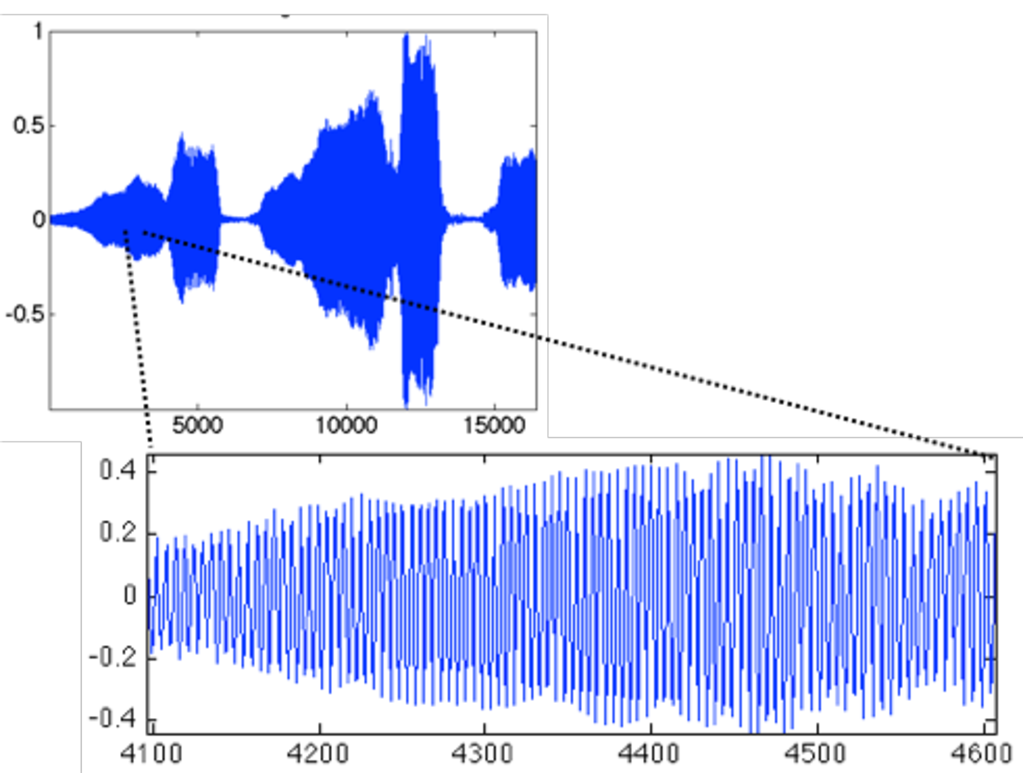
\includegraphics[width=.45\linewidth]{discrete/signal} &
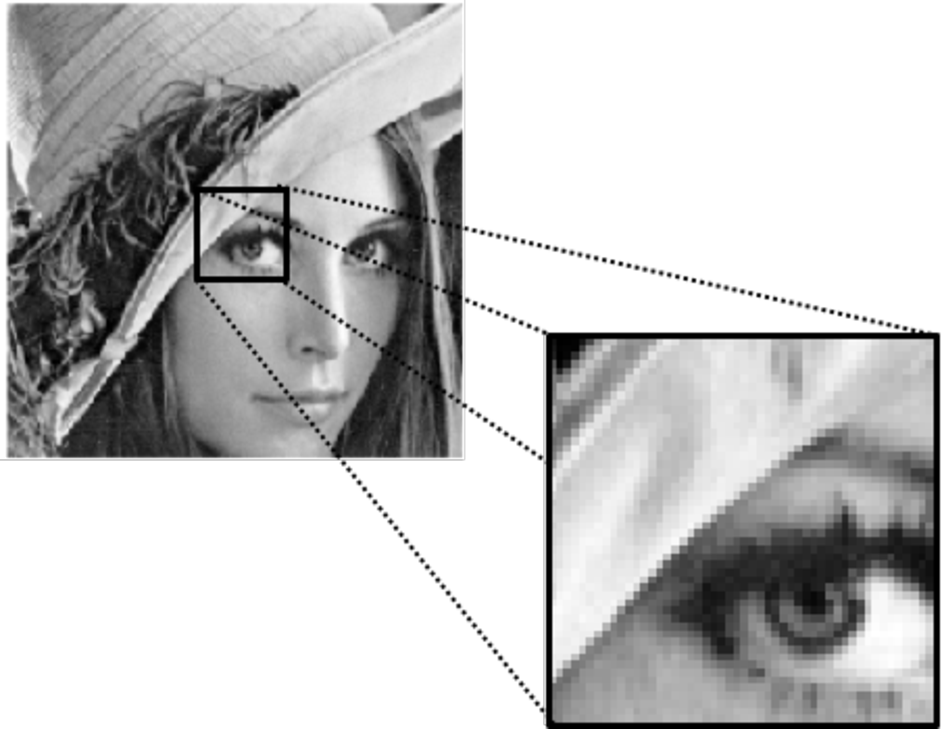
\includegraphics[width=.45\linewidth]{discrete/image}
\end{tabular}
\caption{\label{fig-samples} Examples of a sound signal (1D data) and an image (2D data) discretized.}
\end{figure}

It is the theory developed by Claude Shannon~\cite{Shannon1948} that laid the foundation for sampling (the use of a discrete vector $f$ to faithfully represent a continuous function $\tilde f$) but also those of lossless compression.
%
We will see how current research has made it possible to build on these foundations lossy compression methods (i.e with a slight degradation of the quality), as well as to revisit the conventional sampling to give rise to the idea of compressed sampling.


%%%%%%%%%%%%%%%%%%%%%%%%%%%%%%%%%%%%
\section{Nonlinear Approximation and Compression}


%%%%%
\subsection{Nonlinear Approximation}

The size $Q$ of these data is generally very large (of the order of million for an image, of the billion for a video) and it is necessary to calculate a more economical representation in order to be able to store $f$ or to transmit it on a network.
%
All modern lossy compression methods (MP3, JPEG, MPEG, etc.) use sparse decompositions (that is composed of few non-zero coefficients) in a dictionary $\Psi = (\psi_n)_{n=1}^N$ composed of elemental atoms $\psi_n \in \RR^Q$.
%
It is thus sought to approach $f$ with the aid of a linear combination
\eq{
	f \approx  \Psi x \eqdef \sum_{n=1}^N x_n \psi_n \in \RR^Q
}
where the $x = (x_n)_{n=1}^N \in \RR^N$ are the coefficients that will be stored or transmitted. In order for this representation to be economical, and for storage to take up little space, it is necessary that a maximum of coefficients $x_n$ be zero, so that only the non-zero coefficients have to be stored. Given a budget $M>0$ of non-zero coefficients, the best possible combination is sought in order to approximate $\ell^2$ the initial data. The aim is to solve the optimization problem
\eql{\label{eq-pbm-approx}
	x^\star \in \uargmin{x \in \RR^N} \enscond{  \norm{f - \Psi x}_2  }{ \norm{x}_0 \leq M }
	\qwhereq
	\norm{f}_2^2 \eqdef \sum_{q=1}^Q |f_q|^2.
}
Here we have noted $\norm{x}_0 \eqdef \sharp\enscond{n}{x_n \neq 0}$ the number of non-zero coefficients of $x$, which is a counting measure often referred to by language abuse as the \guill{pseudo-norm} $\ell^0$ (which is not a standard!). This abuse of language will be explained in section~\ref{sec-pb-inv}, see in particular figure~\ref{fig-boules}.

The problem~\eqref{eq-pbm-approx} is in general impossible to solve: it is a combinatorial problem, which, without further hypothesis on $\Psi$, requires the exploration of all combinations of $M$ coefficients non-zero. It has been proved that this problem is indeed NP-difficult~\cite{Natarajan95}.


%%%%%
\subsection{Approximation in an orthonormal basis}

There is however a simple case, which is very useful for compression: this is the case where $\Psi$ is an orthonormal basis of $\RR^Q$, ie $Q = N$ and
\eq{
	\dotp{\psi_n}{\psi_{n'}} = \choice{
		1 \qsiq n = n', \\
		0 \quad\text{sinon.}
	}
	\qwhereq
	\dotp{f}{g} \eqdef \sum_{q=1}^Q f_q g_q.
}
This case is the one most often encountered for data compression, using for example discrete Fourier orthogonal bases, local cosines (used for MP3, JPG and MPG) and wavelets (used for JPEG2000), see the book~\cite{mallat2009a-wav}.
%
In this case, we have the identity of Parseval which corresponds to the decomposition of $f$ in an orthonormal basis
\eql{\label{eq-expansion-bon}
	f = \sum_{n=1}^N \dotp{f}{\psi_n} \psi_n 
	\qetq
	\norm{f - \Psi x}_2^2 = \sum_{n=1}^N | \dotp{f}{\psi_n} - x_n |^2.
}
These formulas show that the solution of~\eqref{eq-pbm-approx} is very simple to calculate.
%
Indeed, to minimize $\norm{f - \Psi x}_2$, for each non-zero $x_n$, one should choose $x_n = \dotp{f}{\psi_n}$.
%
And since we set a maximum budget of $M$ non-zero coefficients, we must choose the $M$ largest coefficients $|\dotp{f}{\psi_n}|$ in the formula~\eqref{eq-expansion-bon}. Mathematically, if we note $|\dotp{f}{\psi_{n_1}}| \geq |\dotp{f}{\psi_{n_2}}| \geq \ldots$ a sorting of the coefficients in descending order, then a $x^\star$ solution of~\eqref{eq-pbm-approx} is given by
\eql{\label{eq-formule-thresh}
x^\star_n = \choice{
\dotp{f}{\psi_{n}} \qsiq \in \{n_1,\ldots, n_M\}, \\
0 \quad\text{otherwise}
}
}

\newcommand{\myPic}[1]{\includegraphics[trim=50 50 30 30,clip,width=.24\linewidth]{approx/#1}}
\begin{figure}\centering
\begin{tabular}{@{}c@{\hspace{1mm}}c@{\hspace{1mm}}c@{\hspace{1mm}}c@{}}
\myPic{cameraman} &
\myPic{cameraman-4} &
\myPic{cameraman-8} &
\myPic{cameraman-16} \\
$f$ & 
$\Psi x^\star, M=N/4$ & 
$\Psi x^\star, M=N/8$ &  
$\Psi x^\star, M=N/16$ 
\end{tabular}
\caption{\label{fig-approx} Approximate Examples $f \approx \Psi x^\star$ with $M = \norm{x^\star}_0$ which varies, for a $f \in \RR^N$ image of $N = 256^2$ pixels.}
\end{figure}


The figure~\ref{fig-approx} shows approximations $f \approx \Psi x^\star$, with a variable number $M = \norm{x^\star}_0$  of coefficients.
%
These approximations are performed using an orthogonal base of wavelets $\Psi$, called the Daubechies 4 base, which are similar to the functions used in the JPEG2000 image compression standard, and are popular because there is a fast algorithm for calculate the scalar products $( \dotp{f}{\psi_{n}} )_n$ with a computation time proportional to $Q$ (see the book~\cite[Chapter 7]{mallat2009a-wav} for a complete description of the theory of wavelets).
%
It can be seen that the quality of the reconstructed image $\Psi x^\star$ degrades when $M$ decreases, but one can still considerably reduce the amount of information to be stored (the $M/Q$ compression ratio is small), while maintaining an acceptable visual quality.
%
This fundamental observation corresponds to the fact (observed in practice) that natural images are very well approximated by a \guill{sparse} linear combination of the form $\Psi x^\star$ with $\norm{x^\star}_0 \leq M$.
%
It is important to note that, although the calculation of $\Psi x^\star$ from $x^\star$ is a linear formula, the calculation of $x^\star$ from $f$ is \textit{non-linear}, as can be seen in the formula~\eqref{eq-formule-thresh}. The transition from $f$ to its approximation $\Psi x^\star$ is called a non-linear approximation.
%
The theoretical justification of this observation is the object of the study of nonlinear approximation theory, which seeks to prove that $\norm{f-\Psi x^\star}$ decreases rapidly when $M$ increases under certain assumptions of regularity over $f$, for instance assuming that the image is piecewise smooth, see~\cite[Chap. 9]{mallat2009a-wav}.

In order to obtain an complete compression algorithm, it is then necessary to use a technique making it possible to convert the $M$ coefficients $(x_{n_1}, \dots, x_{n_2})$ into binary writing and also to store the non-zero indices $(n_1,\ldots, n_M)$. This is done simply using techniques derived from information theory, in particular entropy coding methods, see~\cite[Chap. 10]{mallat2009a-wav}.

%%%%%%%%%%%%%%%%%%%%%%%%%%%%%%%%%%%%%%%%%%%%%
\section{Inverse Problems and Sparsity}
\label{sec-pb-inv}

%%%%%
\subsection{Inverse Problems}

Before $f$ data can be stored, it is most of the time necessary to carry out a preliminary restoration step, which consists in improving the quality of the data from observations of low quality, that is to say --9 of low resolution, possibly blurred , entangled with errors and noisy. In order to take into account the whole chain of data formation, we model mathematically the acquisition process in the form
\eql{\label{eq-fwd-model}
	y = \Phi f + w \in \RR^P
}
where $y \in \RR^P$ are the $P$ observations measured by the device, $w \in \RR^P$ is a measurement noise (unknown), $f \in \RR^Q$ is the image (unknown) that one wishes to recover, and $\Phi : \RR^Q \rightarrow \RR^P$ is an operator modeling the acquisition apparatus, and which is assumed to be ``linear". This means that $\Phi$ may be considered as a (gigantic) matrix $\Phi \in \RR^ (P \times Q) $. It is important to note that most of the time this matrix $\Phi$ is never explicitly stored, it is manipulated implicitly by means of fast operations (convolution, masking, etc.).


\begin{figure} \centering
\begin{tabular}{@{}c@{\hspace{4mm}}c@{\hspace{4mm}}c@{}}
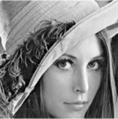
\includegraphics[width=.25\linewidth]{operators/lena-original} &
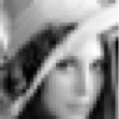
\includegraphics[width=.25\linewidth]{operators/lena-blurring} &
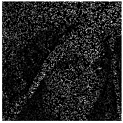
\includegraphics[width=.25\linewidth]{operators/lena-inpainting} \\
Image originale $f$ & $\Phi f$ (flou) & $\Phi f$ (masquage)  
\end{tabular}
\caption{Observation (noiseless, $w=0$) $y=\Phi f$ in the case of a convolution ($\Phi f = \phi \star f$ is a convolution against a low pass filter $\phi$) and missing data  ($\Phi=\diag(\mu_q)_{q=1}^Q$ is a masking operator).  \label{fig-exemple-ip} }
\end{figure}


This model, which may seem rather restrictive (in particular the hypothesis of linearity) makes it possible to model a surprising quantity of situations that one meets in practice. For example,
\begin{itemize}
	\item Denoising: $\Phi = \Id_{\RR^Q} $, $P = Q$ and one is in the (simplest) situation in which one only seeks to remove the noise $w$ ;
	 \item Deconvolution: (see Figure~\eqref{fig-exemple-ip}, center) $\Phi f = \phi \star f$ is a convolution by a filter $\phi$ modeling for example the blur of a camera (either a blur of shake or a blur due to development) ;
	\item Missing data: (see Figure~\eqref{fig-exemple-ip}, right)  $\Phi=\diag(\mu_q)_{q=1}^Q$  is a diagonal masking operator, such as $\mu_q = 1$ if the data indexed by $q$ (for example, one pixel) is observed, and $\mu_q = 0$ if the data is missing;
	 \item tomographic imagery: $\Phi$ is a more complex linear operator, calculating integrals along straight lines (the Radon transform), see \cite[Sect. 2.4]{mallat2009a-wav}.
\end{itemize}
There are many other examples (in medical imaging, seismic, astrophysics, etc.), and in each case, calculating a good approximation of $f$ from $y$ is very difficult. Indeed, with the exception of denoising (ie $\Phi = \Id_{\RR^Q} $), the formula $\Phi^{-1} y = f + \Phi^{-1} w$ can not be used either because $\Phi$ is not invertible (for example for missing data), or because $\Phi$ has very small eigenvalues (for deconvolution or tomography), so that $\Phi^{-1} w$ is going to be very large, and thus $\Phi^{-1} y$ is a very bad approximation of $f$.


%%%%%
\subsection{Sparse Regularization}

To remedy this problem, we need to replace $\Phi^{-1}$ with an approximate \guill{inverse} which takes into account additional assumptions about the $f$ signal we are looking for. Recent methods, which give the best results on complex data, use an approximate inverse which is nonlinear. This may seem contradictory because $\Phi$ is linear, but the use of nonlinear methods is crucial to take advantage of realistic assumptions about complex data such as images.
%
Based on the approximation and compression techniques discussed in the previous section, current methods seek to exploit the fact that one can approach $f$ with a sparse approximation $\Psi x$ with $\norm{x}_0 \leq M$. Given a parameter $M> 0$, we will look to approximate $f$ by $f^\star = \Psi x^\star$ where $x^\star$ is a solution of
\eql{\label{eq-pbm-l0}
	x^\star \in \uargmin{x \in \RR^N} \enscond{\norm{y - \Phi \Psi x}_2}{\norm{x}_0 \leq M}
}
We see that~\eqref{eq-pbm-l0} is quasi-identical to~\eqref{eq-pbm-approx}, except that $f \in \RR^Q$ (unknown) has been replaced by $y\in \RR^P$, and that matrix $\Psi \in \RR^{Q \times N}$ by matrix product $\Phi \Psi \in \RR^{P \times N} $. In the particular case of denoising, $\Phi = \Id_{\RR^Q} $, the problems~\eqref{eq-expansion-bon} and~\eqref{eq-pbm-l0} are equivalent and have the same solution, so that the nonlinear approximation solves the denoising problem .

In the case of any operator $\Phi$, the problem~\eqref{eq-pbm-l0} is however an optimization problem extremely difficult to solve. Indeed, even if $\Psi$ is an orthonormal basis, in general (except in the case of denoising $\Phi = \Id_{\RR^Q}$), the matrix $\Phi \Psi$ is not orthogonal, so that the formula~\eqref{eq-formule-thresh} is not applicable, and~\eqref{eq-pbm-l0} is a NP-difficult combinatorial search problem.


%%%%%
\subsection{$\ell^1$ Regularization}

The approximation of the solutions of the problem~\eqref{eq-pbm-l0} using efficient methods is one of the most active subjects of research in data processing (and more generally in applied mathematics, imagery, statistics and machine learning). There are many methods, including greedy algorithms (see, for example,~\cite{MallatMP}) and convex relaxation methods. We will focus on this second class of methods.
%
One way (heuristic) to introduce these techniques is to replace $\norm{\cdot}_0$ in the~\eqref{eq-pbm-l0} problem with the function $\norm{\cdot}_\al^\al$, which is set to $\al>0$ by
\eq{
	\norm{x}_{\al}^\al \eqdef \sum_{n=1}^N |x_n|^\al.
}
Figure \ref{fig-boules} shows in the (unrealistic but convenient to draw) case of $N = 2$ coefficients, the balls of the $B_\al \eqdef \enscond{x}{\norm{x}_\al \leq 1}$ units associated with these functional $\norm{\cdot}_\al$. It can thus be seen that $B_\al$ \guill{tend} to the \guill{unit ball} associated with the counting measure $\norm{\cdot}_0$ as $\al$ tends to $0$,
\eq{
	B_\al \overset{\al \rightarrow 0}{\longrightarrow} B_0 \eqdef \enscond{ x \in [-1,1]^N }{ \norm{x}_0 \leq 1 },
}
the convergence of these sets (which is well visualized in the figure) being in the sense for example of the Hausdorff distance.
%
The limiting ball $B_0$ is composed of extremely sparse vectors, since they are composed of a single non-zero component.

\begin{figure} \centering
\begin{tabular}{@{}c@{\hspace{1mm}}c@{\hspace{1mm}}c@{\hspace{1mm}}c@{\hspace{1mm}}c@{}}
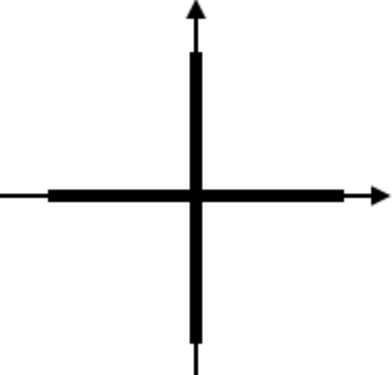
\includegraphics[width=.19\linewidth]{balls/l0} &
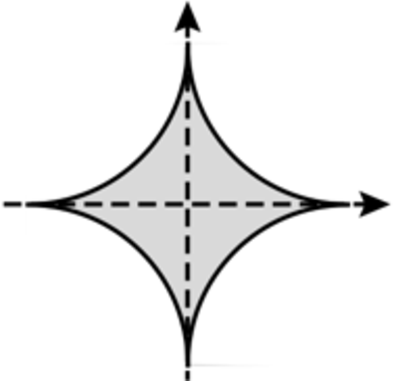
\includegraphics[width=.19\linewidth]{balls/l12} &
\includegraphics[width=.19\linewidth]{balls/l1} &
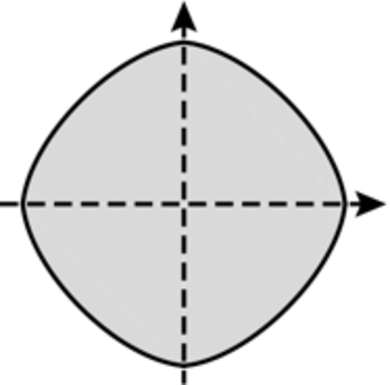
\includegraphics[width=.19\linewidth]{balls/l32} &
\includegraphics[width=.19\linewidth]{balls/l2} \\
$\al=0$ & $\al=1/2$ & $\al=1$ & $\al=3/2$ & $\al=2$
\end{tabular}
\caption{\label{fig-boules} Balls $B_\al$ for different values of $\al$.}
\end{figure}


One then has to take into account two conflicting points to choose a value of $\al$:
\begin{itemize}
	\item In order to have a functional enforcing the sparsity of vectors, we want to use a value of $\al$ as low as possible to replace $\norm{\cdot}_0$ by $\norm{\cdot}_\al$.
	\item In order to calculate the solution of~\eqref{eq-pbm-l0} with $\norm{\cdot}_\al$ instead of $\norm{\cdot}_0$, it is important that the $\norm{\cdot}_\al$ be \textit{convex}. The convexity is indeed essential in order to obtain a problem that is not NP-difficile and to be able to benefit from fast calculation algorithms. These algorithms find an exact solution $x^\star$ in polynomial time or quickly converge to this solution.
\end{itemize}
The convexity constraint of $\norm{\cdot}_\al$ requires that the set $B_\al$ be convex, which equivalently means that $\norm{\cdot}_\al$ must be a \textit{norm}. This imposes that $\al \geq 1$. Taking these two constraints into account leads naturally to the choice  $\al = 1$, so that we consider the convex optimization problem (that is, seeks to minimize a convex function on a convex set)
\eql{\label{eq-pbm-l1}
	x^\star \in \uargmin{x \in \RR^N} \enscond{  \norm{y - \Phi \Psi x}_2  }{ \norm{x}_1 = \sum_{n=1}^N |x_n| \leq \tau }, 
}
so that the retrieved image is defined as $f^\star = \Psi x^\star$.
%
It may be noted that a parameter $\tau>0$ was used here, which plays a role similar to parameter $M$ which appears in~\eqref{eq-pbm-l0}.
%
The question of choosing this parameter $\tau$ is crucial. If the noise $w$ is small, then we want that $\Phi f^\star = \Phi\Psi x^\star$ be close to $y$, and so we will choose $\tau$ big. On the contrary, if the noise $w$ is important, in order to obtain a greater denoising effect, the value of $\tau$ is reduced. The choice of a $\tau$ \guill{optimal} is a difficult search problem, and there is no universal response, the existing strategies strongly depend on the $\Phi$ operator as well as the atoms family~$\Psi$ .

The problem~\eqref{eq-pbm-l1} was initially proposed by engineers in the fields of seismic imaging (see for example~\cite{santosa1986linear}), and it was introduced jointly in signal processing under the name \guill{basis pursuit}~\cite{chen1999atomi} and in statistics under the name \guill{Lasso}~\cite{tibshirani1996regre}.


\begin{figure} \centering
\begin{tabular}{@{}c@{\hspace{4mm}}c@{\hspace{4mm}}c@{}}
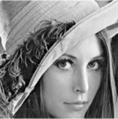
\includegraphics[width=.25\linewidth]{operators/lena-original} &
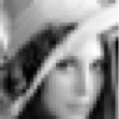
\includegraphics[width=.25\linewidth]{operators/lena-blurring} &
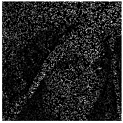
\includegraphics[width=.25\linewidth]{operators/lena-inpainting} \\
$f$ Original & Observations $y$ & Reconstruction $f^\star$
\end{tabular}
\caption{Examples of reconstruction with missing data, $\Phi = \diag(\mu_q)_{q = 1}^Q$ with $\mu_q \in \{0,1\}$ and a number of observed data $\sharp\enscond{q}{\mu_q = 1}=10\%$. \label{fig-inpainting}}
\end{figure}

The problem~\eqref{eq-pbm-l1}, although convex, remains a difficult problem to solve because of the nondifferentiability of $\norm{\cdot}_1$ and large data size ($N$ is very large). This is the price to pay for getting good quality results. As will be explained in the following paragraph, it is in fact the nondifferentiability of $\norm{\cdot}_1$ which makes it possible to obtain sparsity. The development of efficient algorithms to solve~\eqref{eq-pbm-l1} is a very active field of research, and we refer to~\cite[section 6]{2014-vaiter-ps-review} for a review of these methods. Figure~\ref{fig-inpainting} shows an example of missing data interpolation performed by solving~\eqref{eq-pbm-l1} in a $\Psi$ family of translationally invariant wavelets.


%%%%
\subsection{From Intuition to Theory}


The figure~\ref{fig-l1-vs-l2} shows intuitively why the $x^\star$ solution calculated by replacing $\norm{\cdot}_0$ by $\norm{\cdot}_\al$ in~\eqref{eq-pbm-l0} is better (in the sense that it is more sparse) if we choose $\al=1$ (that is, if we solve~\eqref{eq-pbm-l1}) than if we choose $\al = 2$ (a similar conclusion is obtained for other values of $\al> 1$).
%
The figure is made in the (very simple) case of $N = 2$ coefficients and $P = 1$ observations. The crucial point, which makes the solution of~\eqref{eq-pbm-l1} sparse, is that the ball $B_1$ associated with the $\ell^1$ standard is \guill{pointed} so that the $x^\star$ solution is located along the axes. This is not the case for ball $B_2$ associated with standard $\ell^2$, which gives a $x^\star$ solution that is not along the axes, and therefore is not sparing.
%
This phenomenon, already visible in dimension 2, is actually accentuated when the dimension increases, so that the approximation obtained by replacing $\norm{\cdot}_0$ by $\norm{\cdot}_1$ becomes better in large dimension.
%
This phenomenon is called the \guill{blessing of dimensionality} by David Donoho~\cite{DonohoCurse}: although the data become very expensive and complex to treat, there are effective analysis and processing techniques when they are sufficiently sparse.
%
To make this intuition rigorous, however, is difficult, and this is the object of research still in progress for operators $\Phi$ such as convolutions~\cite{candes-towards2013,2015-duval-focm}. The analysis in the case of the operators that one meets for example in medical imaging is an open mathematical problem.


\begin{figure} \centering
\begin{tabular}{@{}c@{\hspace{4mm}}c@{}}
\includegraphics[width=.35\linewidth]{l1-vs-l2/l1} &
\includegraphics[width=.35\linewidth]{l1-vs-l2/l2} \\
$\ell^1$ minimisation &  $\ell^2$ minimisation
\end{tabular}
\caption{Comparison of the minimization with constraints of type $\norm{x}_\al \leq \tau$ for $\al \in \{1,2\}$.
%
A $x^\star$ solution is obtained when a tube $\enscond{x}{\norm{\Phi x-y} \leq \epsilon}$ is sufficiently large (ie gradually growing $\epsilon$) as it is tangent in $x^\star$ to the ball $\enscond{x}{\norm{x}_\al \leq \tau}$. \label{fig-l1-vs-l2}}
\end{figure}



%%%%%%%%%%%%%%%%%%%%%%%%%%%%%%%%%%%%%%%%%%%%%
\section{Compressed sampling}

There exists a particular class of operators $\Phi$ for which it is possible to analyze very precisely the performances obtained when we solve~\eqref{eq-pbm-l1}. This is the case where $\Phi$ is drawn randomly according to some distributions of random matrices. Using random matrices may seem strange, because the operators mentioned above (convolution, tomography, etc.) are not at all.
%
In fact, this choice is motivated by a concrete application proposed jointly by Cand�s, Tao and Romberg~\cite{candes2006stable} as well as Donoho~\cite{donoho2006compressed}, and which is commonly called \guill{compressed sensing}.


%%%%
\subsection{Single Pixel Camera}

In order to illustrate the exposition, we will discuss the \guill{single pixel camera} prototype developed at Rice University~\cite{DuarteSinglePixel}, and which is illustrated by the figure~\ref{fig-single-pixel} (left).
%
It is an important research problem of developing a new class of cameras allowing to obtain both the sampling and the compression of the image. Instead of first sampling very finely (ie with very large $Q$) the analog signal $\tilde f$ to obtain a $f \in \RR^Q$ image then compressing enormously (ie with $M$ small) using~\eqref{eq-formule-thresh}, we would like to dispose directly of an economic representation $y \in \RR^P$ of the image, with a budget $P$ as close to $M$ and such that one is able to \guill{decompress} $y$ to obtain a good approximation of the image $f$.

The \guill{single-pixel} hardware performs the compressed sampling of an observed scene $\tilde f$ (the letter \guill{R} in Figure~\ref{fig-single-pixel}), which is a continuous function indicating the amount of light $\tilde f(s)$ reaching each point $s \in \RR^2$ of the focal plane of the camera.
%
To do this, the light is focused against a set of $Q$ micro-mirrors aligned on the focal plane. These micro-mirrors are not sensors. Unlike conventional sampling (described in Section~\ref{sec-sampling}), they do not record any information, but they can each be positioned to reflect or absorb light.
%
To obtain the complete sampling/compression process, one very quickly changes $P$ times the configurations of the micro-mirrors. For $p = 1,\dots, P$, one sets $\Phi_{p, q} \in \{0,1\}$, depending on whether the micromirror at position $q$ has been placed in the absorbing (0) or reflective (value 1) position at step $p$ of the acquisition.
%
The total light reflected at step $p$ is then accumulated into a single sensor (hence the name \guill{single pixel}, in fact it is rather a \guill{single sensor}), which achieves a linear sum of the reflected intensities to obtain the recorded $y_p \in \RR$ value.
%
In the end, if the light intensity arriving on the surface $c_q$ of the mirror indexed by $f_q = \int_{c_q} \tilde f(s) \text{d} s$ is denoted (as in the~\ref{sec-sampling} section) as $q$, the equation that links the discrete image $f \in \RR^Q$ \guill{seen through the mirrors} to the $P$ measures $y \in \RR^P$ is
\eq{
	\foralls p = 1,\ldots,P, \quad
	y_p = \sum_q \Phi_{p,n} \int_{c_n} \tilde f(s) \text{d} s = (\Phi f)_p, 
}
which corresponds exactly to~\eqref{eq-fwd-model}.
%
It is important to note that the mirrors do not record anything, so in particular the $f$ discrete image is never calculated or recorded, since the device directly calculates the compressed representation $y$ from the analog signal $\tilde f$.
%
The term $w$ models here the acquisition imperfections (measurement noise). The compressed sampling therefore corresponds to the transition from the observed scene $\tilde f$ to the compressed vector $y$. The \guill{decompression} corresponds to the resolution of an inverse problem, whose goal is to find a good approximation of $f$ (the discrete image \guill{ideal} as seen by the micro-mirrors) from $y$.

\begin{figure} \centering
\begin{tabular}{@{}c@{\hspace{1mm}}c@{\hspace{1mm}}c@{}}
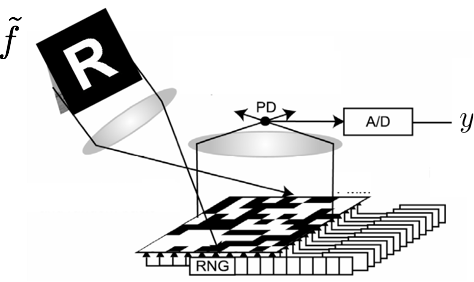
\includegraphics[width=.45\linewidth]{single-pixel/single-pixel-schema}&

\includegraphics[width=.25\linewidth]{single-pixel/reconstruction-1}&

\includegraphics[width=.25\linewidth]{single-pixel/reconstruction-6}\\
Diagram of the device & $f$ & $f^\star$, $P/Q = 6$
\end{tabular}
\caption{Left: diagram of the single-pixel acquisition method.
%
Center: image $f \in \RR^Q$ \guill{ideal} observed in the focal plane of the micro-mirrors.
%
Right: image $f^\star = \Psi x^\star$ reconstructed from observation $y \in \RR^P$ with a compression factor $P / Q = 6$.
\label{fig-single-pixel}}
\end{figure}




%%%%
\subsection{Theoretical Guarantees}

An important feature of this inverse problem is that one can choose, as desired, the configurations of the micro-mirrors, which amounts to saying that one can choose freely the matrix $\Phi \in \{0,1\}^{P \times Q} $. The question is therefore to make the best choice, so that the inverse problem can be solved effectively. If we make the hypothesis that the signal $f$ to be reconstructed is compressible in an orthonormal basis $\Psi$ (that is to say that $f \approx \Psi x_0$ with $M \eqdef \norm{x_0}_0$ small) then several recent works, starting with~\cite{candes2006stable,donoho2006compressed}, showed that method~\eqref{eq-pbm-l1} is effective if $\Phi$ is chosen as a realization of some random matrices. For the single-pixel camera, each $\Phi_{p, n}$ can then be randomly drawn with a probability of $1/2$ for the values $0$ and $1$.
%
In practice, a pseudo-random generator is used, so that both the person who compresses the data and the person who is going to decompress them knows the matrix $\Phi$ perfectly (because they can communicate the seed of the generator).
%
The figure~\ref{fig-single-pixel} (right) shows an example of reconstruction obtained for the case of the single-pixel apparatus with such a random choice of matrix $\Phi$, with $\Psi$ a translation-invariant family of wavelets (see~\cite[Section 5.2]{mallat2009a-wav} for a description of this family).

It has been shown by~\cite{candes2006stable,donoho2006compressed} that there exists a constant $C$ such that if $f = \Psi x_0$ where $x_0$ are the coefficients of the image to be retrieved, where $\Psi$ is an orthogonal basis therefore in particular $Q = N$), and if the number $P$ of measurements satisfies
\eql{\label{eq-cs-contrainte}
\frac{P}{M} \geq C \log\pa{\frac{N}{M}} \qwhereq M \eqdef \norm{x_0}_0
}
then a solution $f^\star = \Psi x^\star$ computed by~\eqref{eq-pbm-l1} tends to $f$ when the $w$ noise tends to $0$ and $\tau$ tends to$ +\infty$. This result is true \guill{with high probability} on the random drawing of the matrix $\Phi$, that is to say a probability tending rapidly towards 1 when $N$ increases. In particular, if there is no noise, $w = 0$, taking $\tau \rightarrow + \infty$, the method makes it possible to find exactly $f$ if $P$ satisfies~\eqref{eq-cs-contrainte}.
%
This theory also allows to take account of \guill{compressible} data, ie if we only assume that $f$ is close to (but not necessarily equal to) $\Psi x_0$ with $M \eqdef \norm{x_0}_0$ small.

Intuitively, this theoretical result means that compressed sampling can do almost \guill{as well} by calculating $\Psi x^\star$ from $y$ (solving~\eqref{eq-pbm-l1}) than a usual compression method (MP3, JPEG , JPEG2000, MPEG, etc.) that would know exactly the $f$ signal and calculate the best approximation $\Psi x_0$ with $M \eqdef \norm{x_0}_0$ coefficients (solving~\eqref{eq-pbm-approx} via the formula~\eqref{eq-expansion-bon}).
%
The precise meaning of the qualifier \guill{equally} corresponds to the $C \log(N/M)$ multiplying factor, which bounds $P/M$. This factor corresponds to the \guill{extra cost} of the compressed sampling method (which calculates $P$ measurements) compared to a usual compression method (which calculates $M$ coefficients).
%
Despite this additional cost, the compressed sampling method has many advantages: saving time and energy (at the same time sampling and compression), \guill{democratic} coding (all $y_n$ coefficients play the same role, and therefore none has a dominant role, unlike the coding of the coefficients of $x_0$ which have an importance proportional to their amplitude), coding automatically encrypted (if $\Phi$ is not known, $f$ can not be found from $y$ ). The value of the $C$ constant depends on the meaning given to \guill{with high probability}. If this probability bears only $\Phi$, but must be true for all $x_0$ (worst case analysis), then it is very large (see~\cite{dossal-laa-09}). If, on the other hand, if the high probability is both on $\Phi$ and $x_0$ (so that the theoretical result is true for almost all the signals) then it can be shown that for example, for $N/P = 4$, we have $C \log (N / M) \sim 4$ (see~\cite{chandrasekaran2012convex}), which remains a significant overhead but is acceptable for some applications.

The \guill{single pixel} camera is a particular application of the compressed sampling technique. Applications to photography are limited because the CCD sensors of cameras are powerful and inexpensive. Compressed sampling is likely to have an impact on applications where measurements are difficult to acquire or costly. Another source of potential applications is medical imaging, for example by magnetic resonance imaging (MRI). In these fields, however, it is impossible to obtain totally random matrices, so that the theory of compressed sampling can not be applied directly. Encouraging results on these applications have however been obtained, see for example~\cite{AdcockBreaking,Chauffert14}.


%%%%%%%%%%%%%%%%%%%%%%%%%%%%%%%%%%%%%%%%%%%%%
\section*{Conclusion}

Recent advances in data analysis have made it possible to extend the scope of compression in order to deal with difficult inverse problems in imaging, but also in other fields (recommendation system, network analysis, etc.). These advances have been made possible by the use of a very broad spectrum of techniques in applied mathematics, covering both harmonic analysis, nonlinear approximation, non-smooth optimization and probability, but also analysis and PDEs (which were not mentioned in this article). Sparse methods associated with $\ell^1$ regularization are only the tip of the iceberg, and more advanced regularizations make it possible to obtain better results by taking into account the complex geometric structures of the data. For more details on these latest advances, we recommend reading the article~\cite{2014-vaiter-ps-review}, as well as visiting the web site \guill{Numerical Tours of Signal Processing}~\cite{2011-peyre-cise}, which features many computer codes to carry out the numerical experiments presented here, as well as many others.

%%%%%%%%%%%%%%%%%%%%%%%%%%%%%%%%%%%%%%%%%%%%%
\section*{Acknowledgments}

I would like to thank Charles Dossal, Jalal Fadili, Samuel Vaiter, St�phane Seuret and the anonymous reviewer for their invaluable help.



% !TEX root = ../TransportFR.tex


\newcommand{\Blu}[1]{{\color{blue}#1}}
\newcommand{\Red}[1]{{\color{red}#1}}
\newcommand{\iC}{\Red{i}}
\newcommand{\jC}{\Blu{j}}
\newcommand{\aC}{\Red{a}}
\newcommand{\bC}{\Blu{b}}


\ifdefined\otarticle
\newcommand{\myparagraph}[1]{\subsection{#1}}
\else
\newcommand{\myparagraph}[1]{\paragraph{#1}}
\chapter{Le transport optimal numérique et ses applications}
\fi

\label{chap-ot}


%%%%%%%%%%%%%%%%%%%%%%%%%%%%%%%%%%%%%%%%%%%%%%
\section{Le Transport Optimal de Monge}

Gaspard Monge, en plus d'être un grand mathématicien, a participé activement à la révolution Française, et a créé l'\'Ecole Polytechnique ainsi que l'\'Ecole Normale Supérieure. Motivé par des applications militaires, il a formulé en 1781 le problème du transport optimal~\cite{Monge1781}~: il s'est posé la question du calcul de la façon la plus économique de transporter de la terre entre deux endroits pour faire des remblais. Dans son texte original, il a fait l'hypothèse que le coût du déplacement d'une unité de masse est égal à la distance parcourue, mais on peut utiliser n'importe quel coût adapté au problème à résoudre. 

%%%%%%%%%%%%%%%%%%%%%%%%%%%%%%%%%%%%%%%%%%%%%%%%%%%%%
\myparagraph{Le problème de Monge}

Pour illustrer le problème et sa formulation mathématique, intéressons-nous à la façon optimale de distribuer les croissants depuis les boulangeries vers les cafés, le matin dans Paris. Pour simplifier, nous allons supposer qu'il y a uniquement six boulangeries et cafés, que l'on peut voir à la figure~\ref{fig:image-cafe} (les boulangeries sont en \Red{rouge} et les cafés en \Blu{bleu}). 
%
On suppose que toutes les boulangeries produisent le même nombre de croissants et que tous les cafés demandent également ce même nombre de croissant.
%
Le coût à minimiser est le temps total des trajets, et l'on note $C_{\iC,\jC}$ le temps entre la boulangerie $\iC \in \{1,\ldots,6\}$  et le café $\jC \in \{1,\ldots,6\}$. Par exemple, on a $C_{\Red{3},\Blu{4}}=10$, ce qui signifie qu'il y a dix minutes de trajet entre la boulangerie numéro $\Red{3}$ et le café numéro $\Blu{4}$. 

\begin{figure}\centering
    \begin{tabular}{@{}c@{\hspace{1mm}}c@{\hspace{4mm}}c@{\hspace{1mm}}c@{}}
        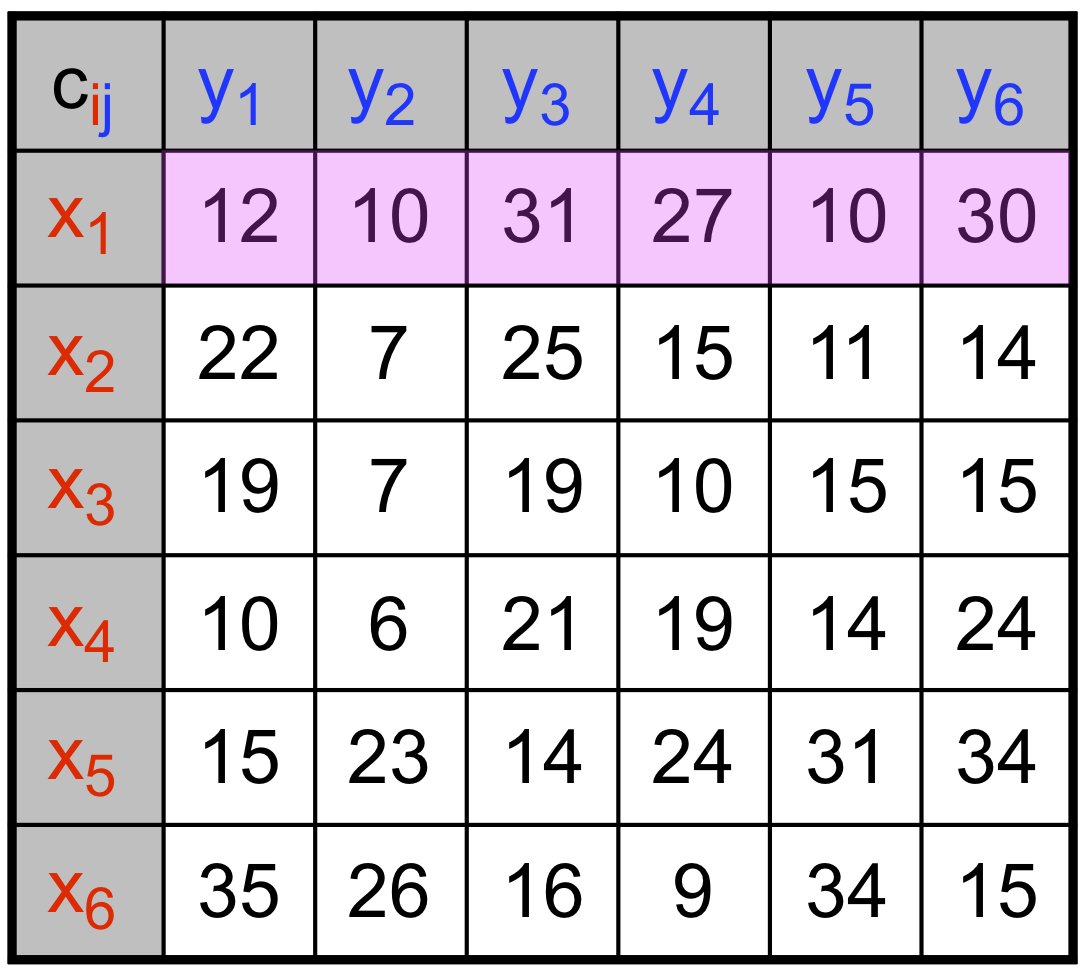
\includegraphics[width=.22\linewidth]{transport/cafe-paris/map-paris-0-couts} 
        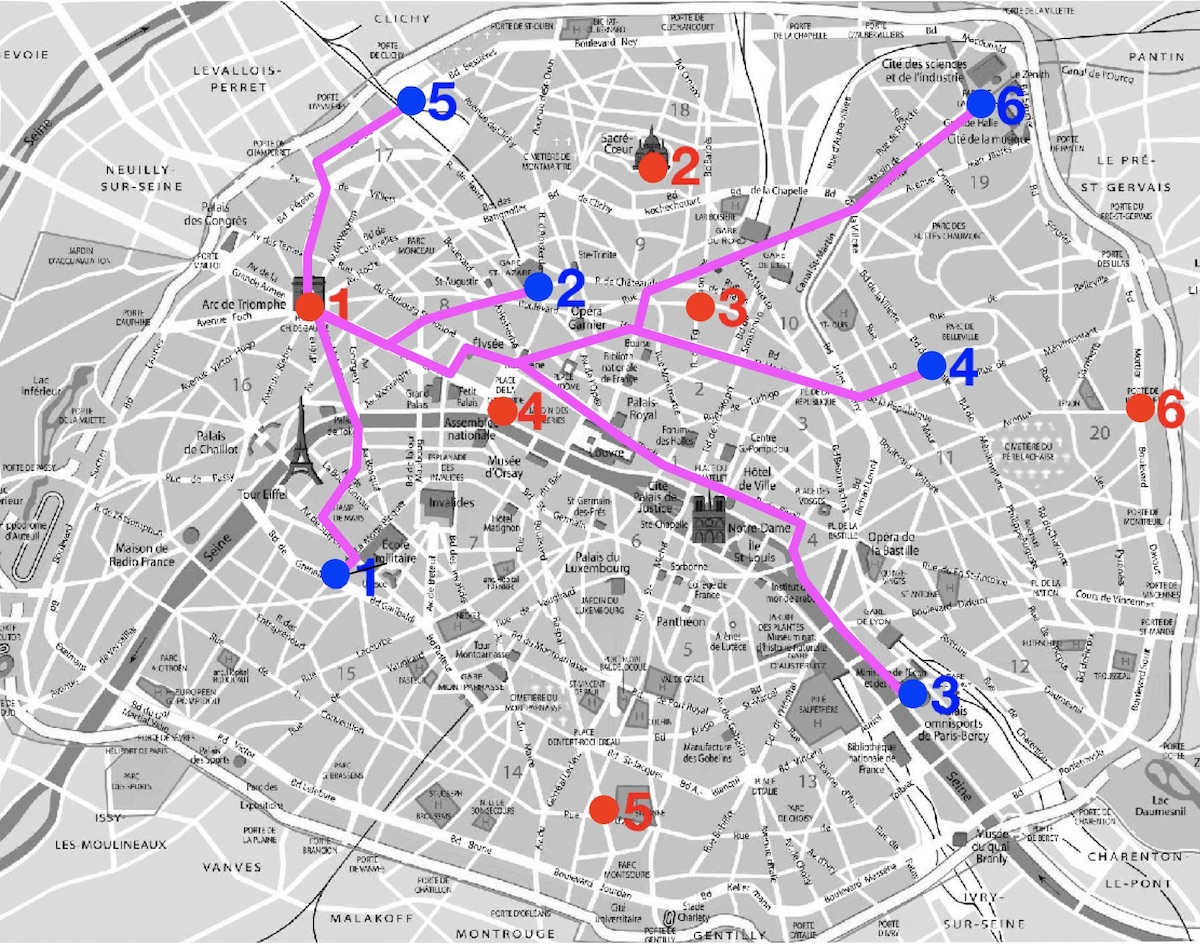
\includegraphics[width=.27\linewidth]{transport/cafe-paris/map-paris-0} 
        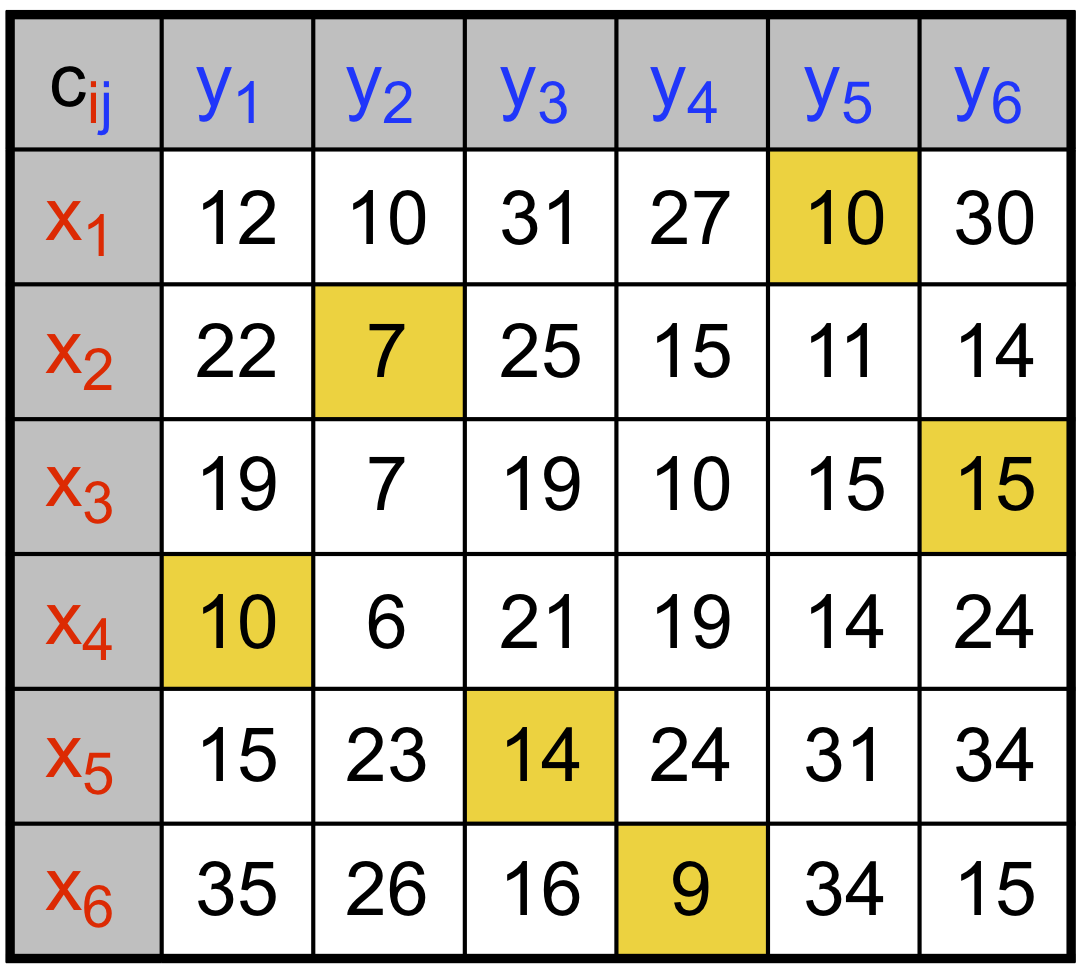
\includegraphics[width=.22\linewidth]{transport/cafe-paris/map-paris-1-couts} 
        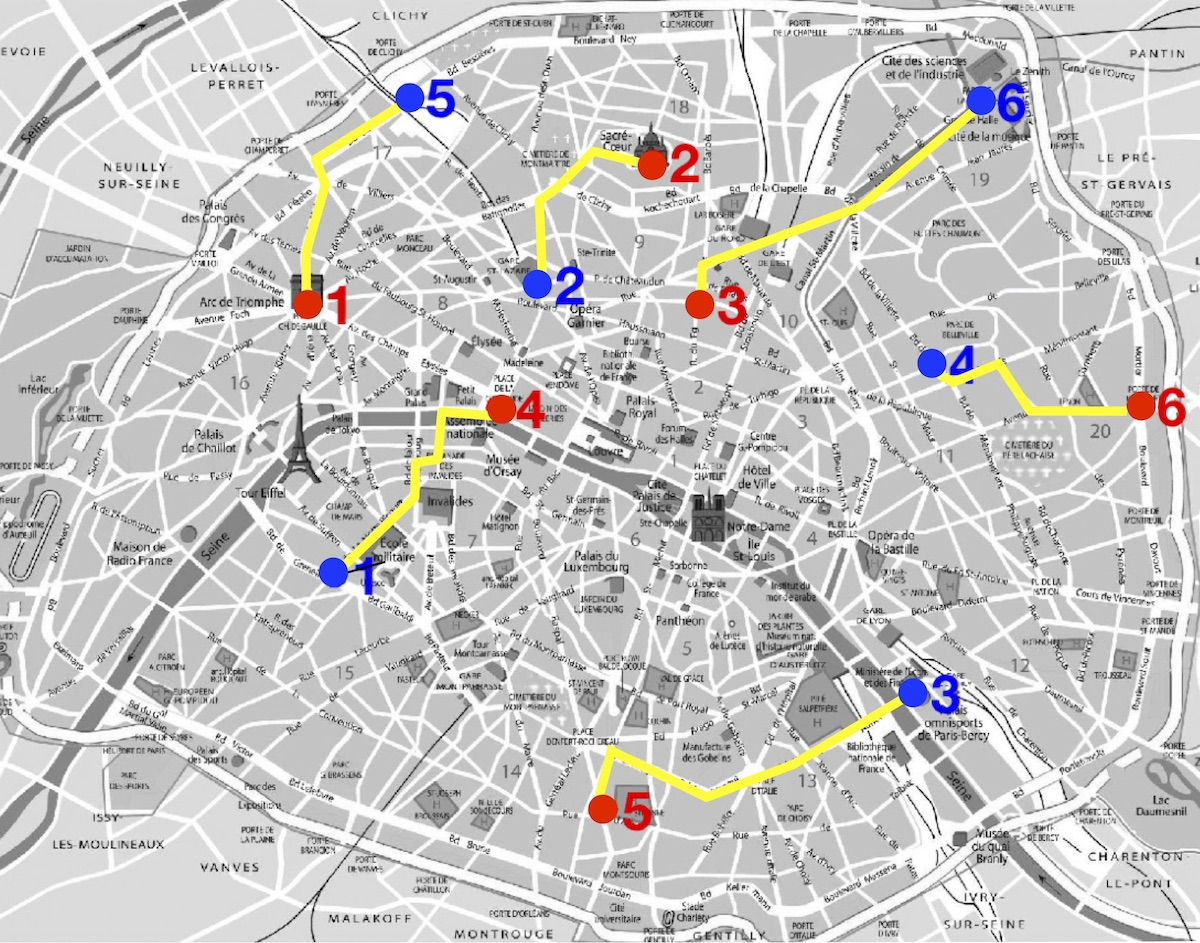
\includegraphics[width=.27\linewidth]{transport/cafe-paris/map-paris-1} 
    \end{tabular}
    \caption{\label{fig:image-cafe} Matrice de coût et connexions associées. Gauche : une ligne de la matrice coût. Droite : un exemple particulier de permutation. } 
\end{figure}

Afin de satisfaire la contrainte d'approvisionnement (que l'on appelle aussi la conservation de la masse), il faut que chaque boulangerie soit connectée à un et un seul café. Comme il y a le même nombre de boulangeries que de cafés, ceci implique que chaque café est également connecté à une et une seule boulangerie. On va noter 
\eq{    
    \si : \iC \in \{1,\ldots,6\} \longmapsto \jC \in \{1,\ldots,6\}
}
un tel choix de connexions. 
%
Les deux images de droite de la figure~\ref{fig:image-cafe} illustrent l'exemple
\eql{\label{eq-bijection-exmp}
    \si(\Red{1})=\Blu{5}, \;
    \si(\Red{2})=\Blu{2}, \;
    \si(\Red{3})=\Blu{6}, \;
    \si(\Red{4})=\Blu{1}, \;
    \si(\Red{5})=\Blu{3}, \;
    \si(\Red{6})=\Blu{4}.
}  
La contrainte de conservation de masse signifie que $\si$ est une bijection de l'ensemble $\{1,\ldots,6\}$ dans lui-même. On dit aussi que $\si$ est une permutation. 

Le coût de transport associé à une telle bijection est la somme des coûts $C_{\iC,\si(\iC)}$ sélectionnés par la permutation $\si$, c'est-à-dire 
\eql{\label{eq:cout}
    \text{Coût}(\si) \eqdef 
        C_{\Red{1},\si(\Red{1})} + 
        C_{\Red{2},\si(\Red{2})} + 
        C_{\Red{3},\si(\Red{3})} + 
        C_{\Red{4},\si(\Red{4})} + 
        C_{\Red{5},\si(\Red{5})} + 
        C_{\Red{6},\si(\Red{6})}. 
}
Par exemple, pour la bijection~\eqref{eq-bijection-exmp} montrée à la figure~\ref{fig:image-cafe}, on obtient comme coût
\eq{
    C_{\Red{1},\Blu{5}} + 
    C_{\Red{2},\Blu{2}} + 
    C_{\Red{3},\Blu{6}} + 
    C_{\Red{4},\Blu{1}} + 
    C_{\Red{5},\Blu{3}} + 
    C_{\Red{6},\Blu{4}} = 
    10 + 7 + 15 + 10 + 14 + 9 = 65. 
}


Le problème de Monge consiste à chercher une permutation $\si$ qui a le coût minimum, c'est-à-dire résoudre le problème d'optimisation
\eql{\label{eq:monge}
    \umin{\si \in \Si_6} \text{Coût}(\si), 
}
où 
l'on a noté $\Si_6$ 
l'ensemble des permutations de l'ensemble $\{1,\ldots,6\}$.

\begin{figure}\centering
    \begin{tabular}{@{}c@{\hspace{1mm}}c@{\hspace{1mm}}c@{\hspace{1mm}}c@{}}
        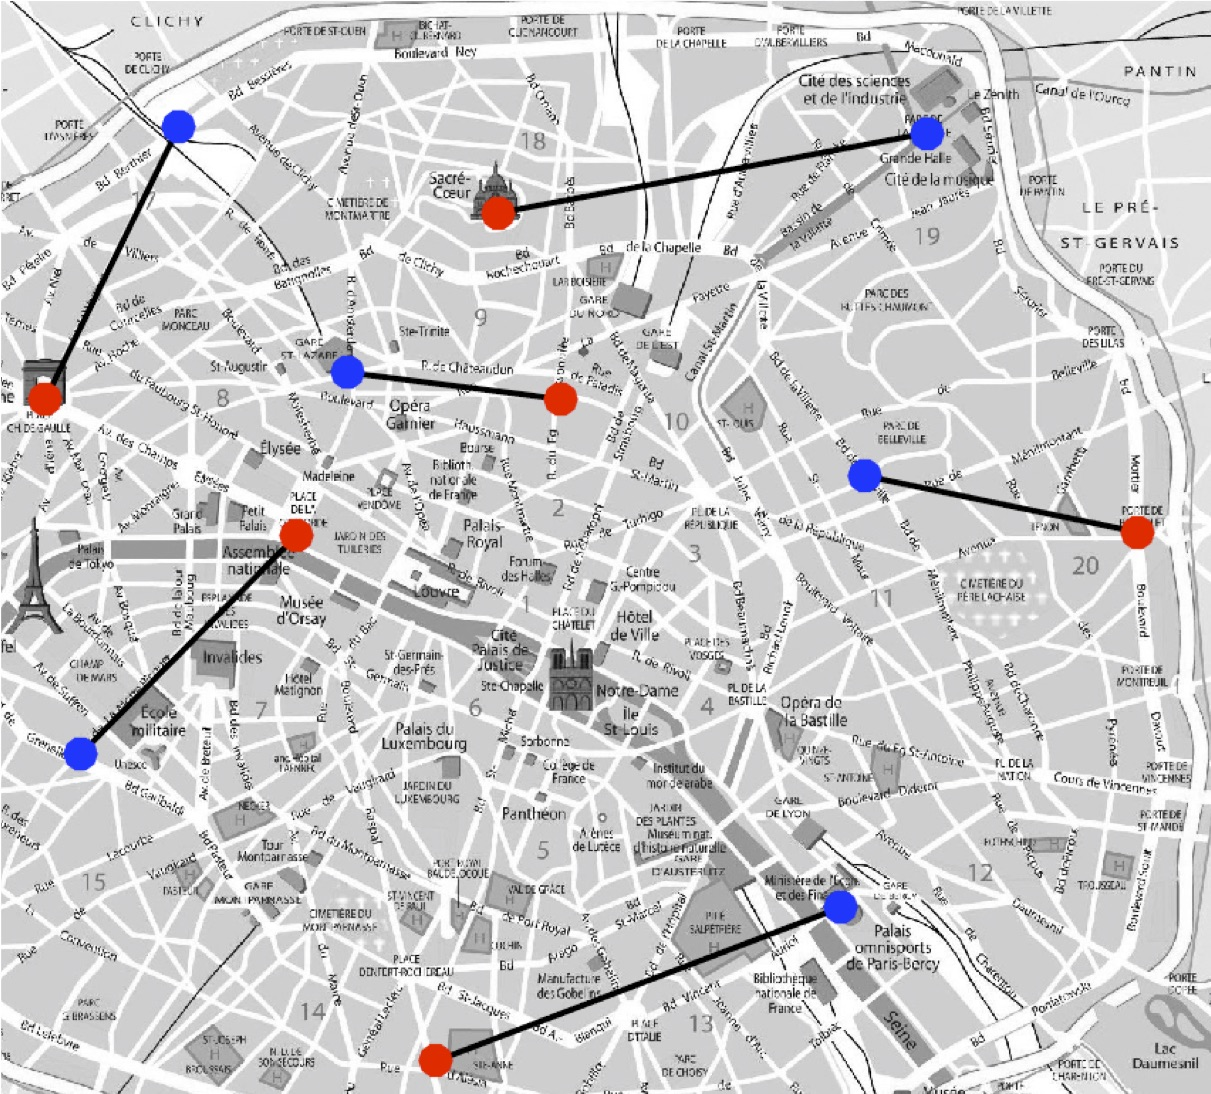
\includegraphics[width=.22\linewidth]{transport/cafe-paris/ordre-croissant-64}&
        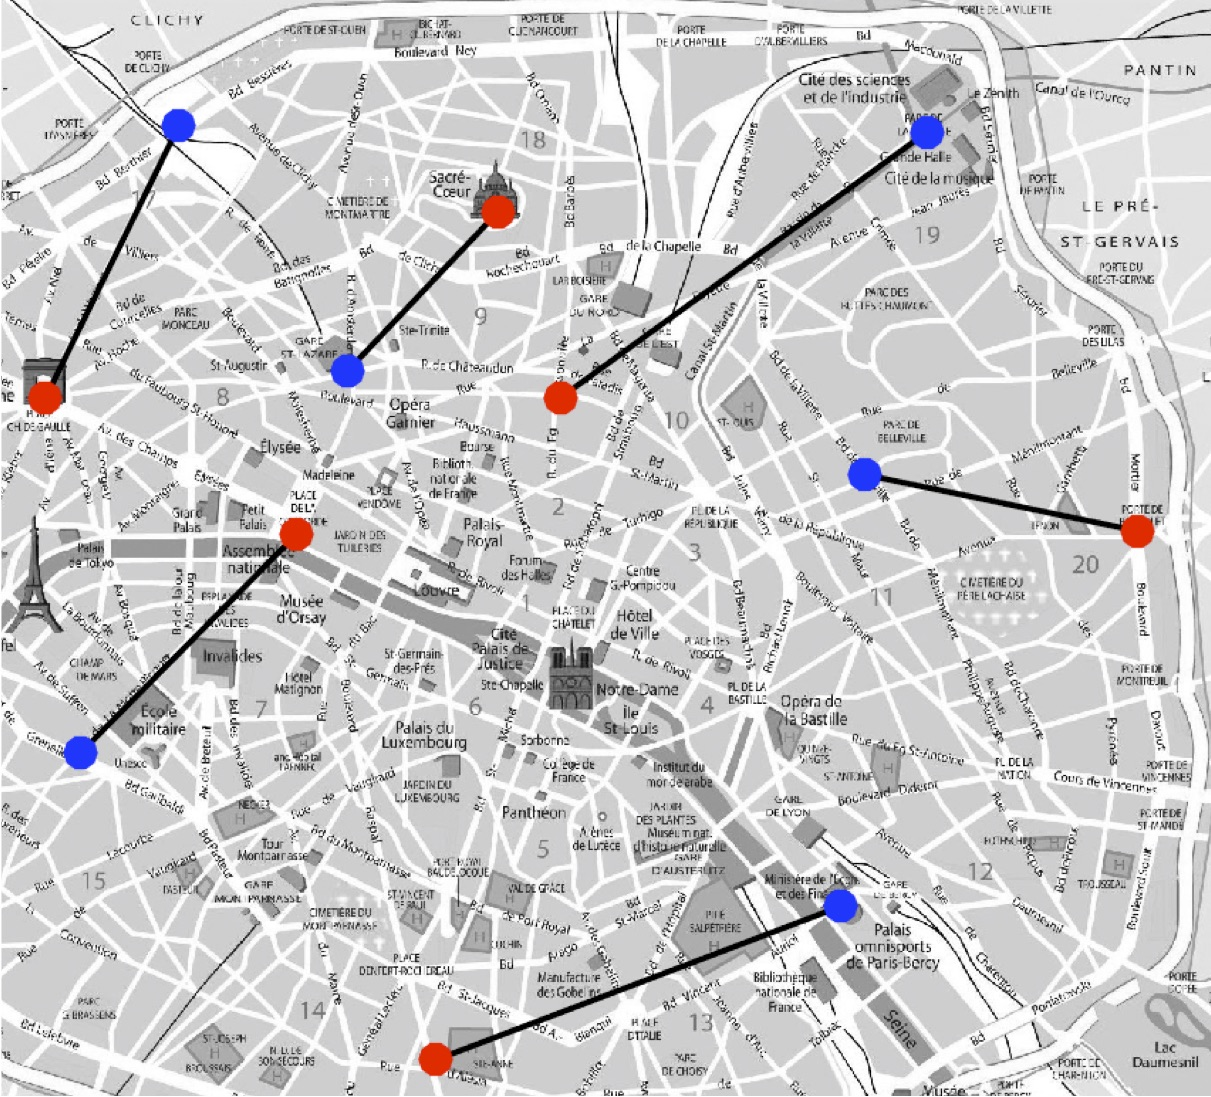
\includegraphics[width=.22\linewidth]{transport/cafe-paris/ordre-croissant-65}&
        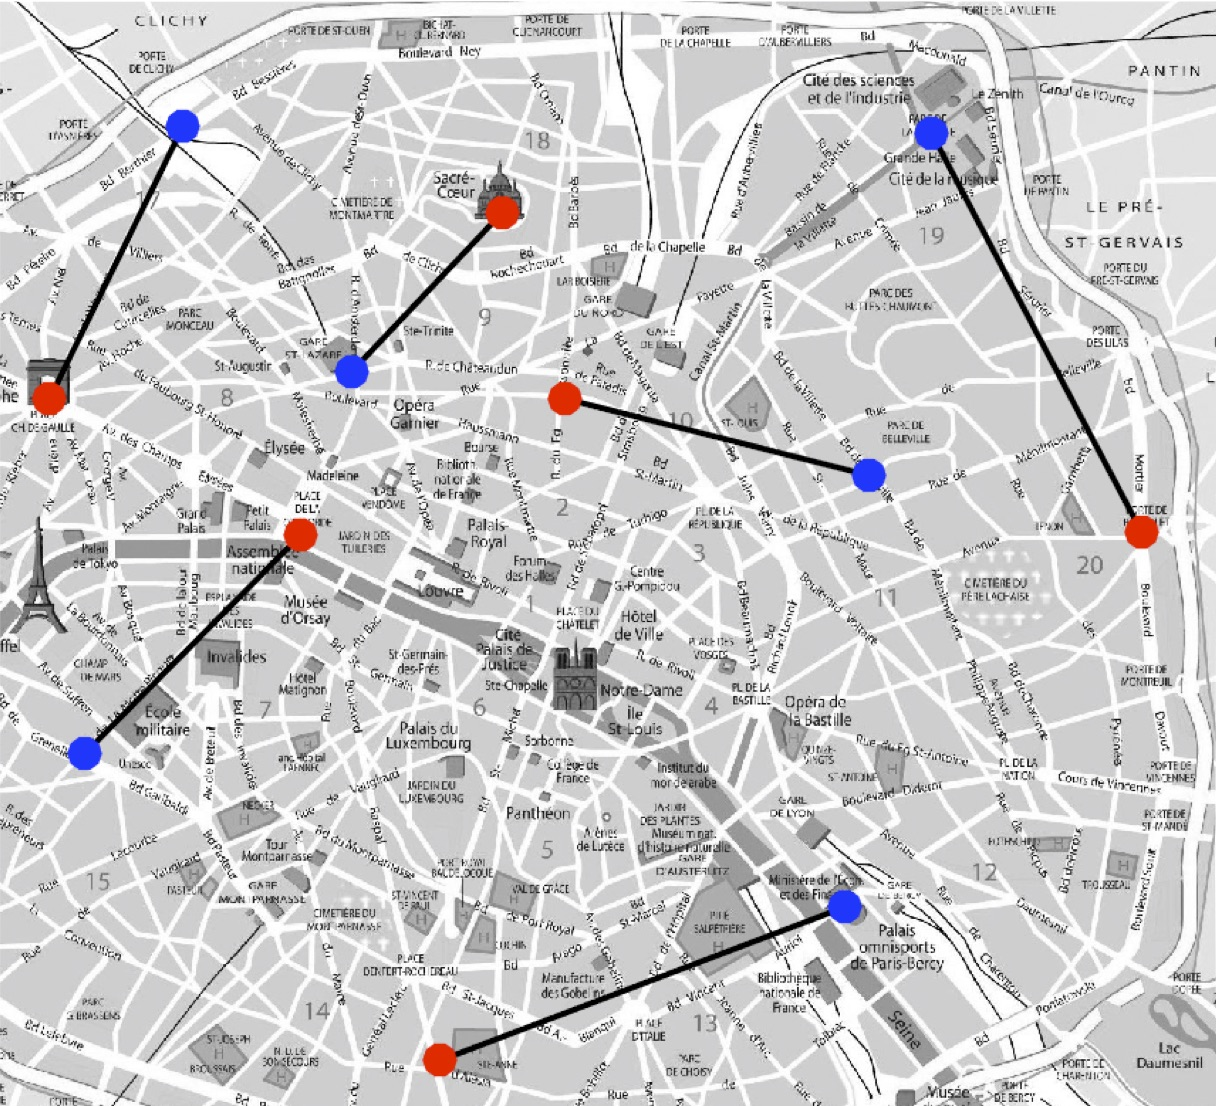
\includegraphics[width=.22\linewidth]{transport/cafe-paris/ordre-croissant-66}&
        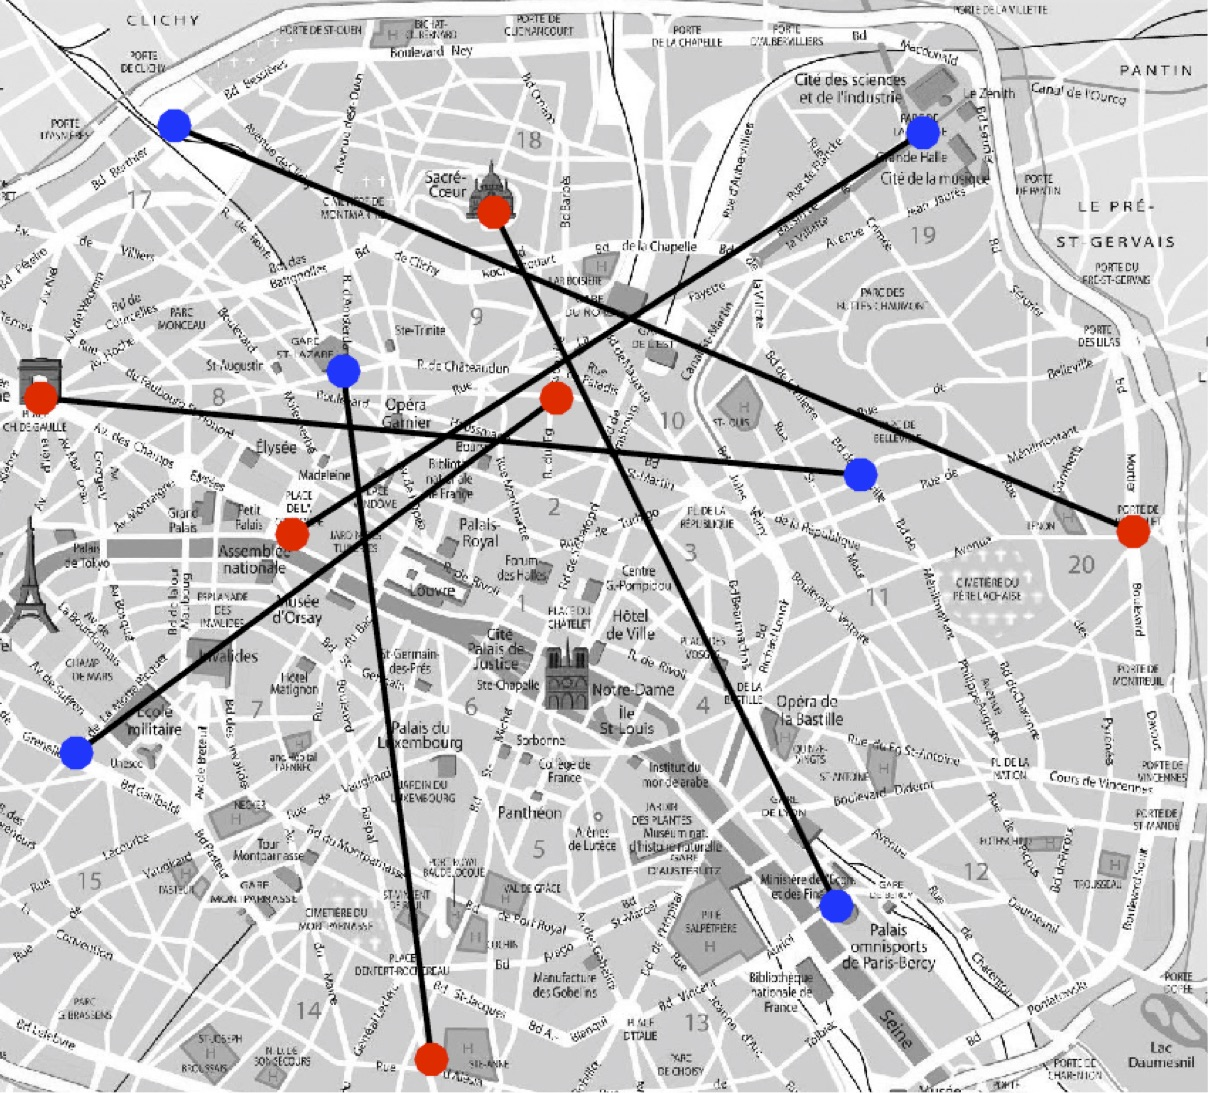
\includegraphics[width=.22\linewidth]{transport/cafe-paris/ordre-croissant-152}\\
        Coût=64 &  
        Coût=65 &  
        Coût=66 &  
        Coût=152
    \end{tabular}
    \caption{\label{fig:ordre-croissant} Exemples de permutations avec différent coûts. } 
\end{figure}

La figure~\ref{fig:ordre-croissant} montre que la permutation~\eqref{eq-bijection-exmp} n'est pas la meilleure : il existe par exemple une autre permutation qui a un coût de 64. Mais est-ce la meilleure ? Il se trouve que oui, on peut en effet tester sur un ordinateur toutes les permutations de  $\{1,\ldots,6\}$ et calculer leur coût. Combien y a-t-il de permutations au total ? Pour effectuer ce dénombrement, on voit qu'il y a six choix d'affectation possible de $\Red{1}$ à  $\si(\Red{1}) \in \{\Blu{1,\ldots,6}\} $, puis cinq choix possibles pour affecter $\Red{2}$ à $\si(\Red{2}) \in  \{ \Blu{1,\ldots,6 } \}  - \{ \si(\Red{1}) \}$, et ainsi de suite. Le nombre total de possibilités est donc $6 \times 5 \times 4 \times 3 \times 2 \times 1 = 720$ que l'on note $6!$. Si l'on considère un nombre $n$ de boulangeries, alors le nombre de permutations à tester pour trouver la meilleure est $n! =n \times (n-1) \times \cdots \times 2 \times 1$. Ce nombre croît extrêmement vite avec $n$, par exemple $70! \approx 1,198 \times 10^{100}$, à comparer avec les $10^{11}$ neurones dans le cerveau et les $10^{79}$ atomes dans l'univers. Cette stratégie de recherche exhaustive n'est donc possible que pour de toute petites valeurs de $n$. 


\begin{figure}\centering
    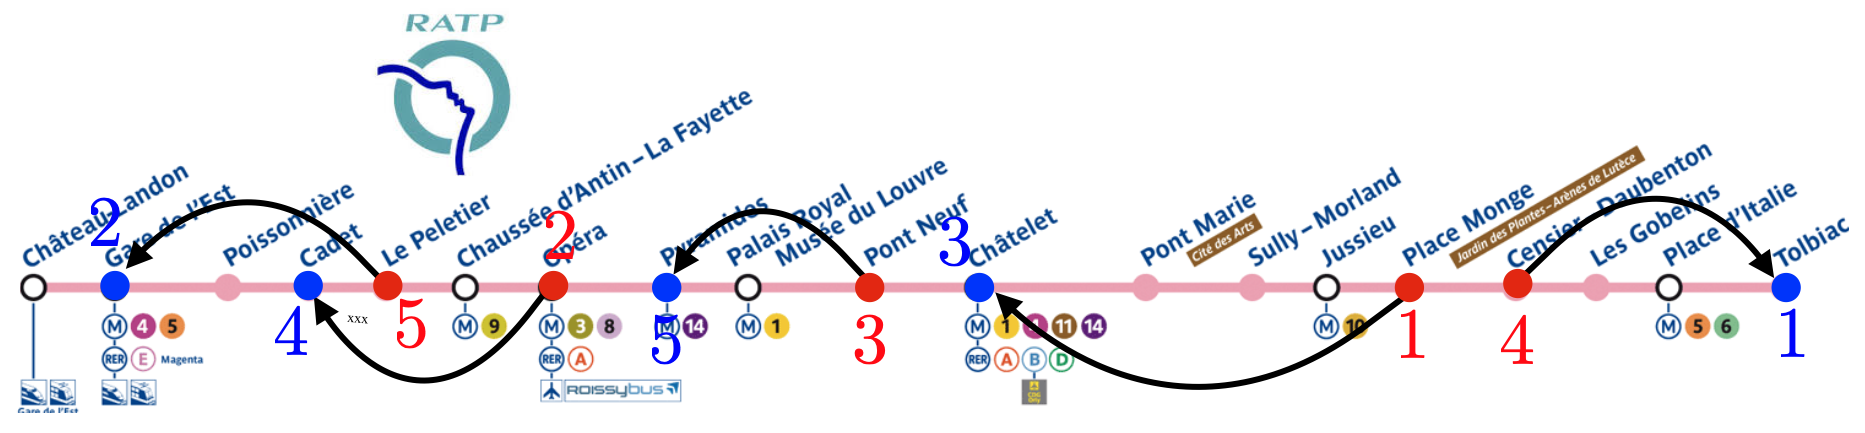
\includegraphics[width=.9\linewidth]{transport/metro/plan-metro}
    \caption{\label{fig:metro} Le transport optimal en 1D le long d'une ligne de métro. La bijection optimale est  
    $\si : (\Red{1,2,3,4,5}) \mapsto (\Blu{3,4,5,1,2})$. } 
\end{figure}

%%%%%%%%%%%%%%%%%%%%%%%%%%%%%%%
\myparagraph{En 1D et 2D}

% ENLEVE : % La section~\ref{sec-kanto} explique comment des avancées mathématiques ont permis de développer des techniques efficaces pour calculer un transport optimal $\si$ même pour de grandes valeurs de $n$. Mais il aura fallu attendre près de 200 ans pour y arriver. Dans quelques rares cas, on peut cependant calculer le transport optimal de façon simple. 

Il aura fallu près de 200 ans pour que des idées nouvelles émergent pour calculer efficacement un transport optimal $\sigma$ même pour des grandes valeurs de $n$. Avant d'expliquer ces avancées mathématiques, commençons par un cas dans lequel le transport optimal se calcule facilement.
%
Le cas le plus élémentaire est lorsque les points à apparier sont le long d'un axe 1D, par exemple si les cafés et les boulangeries sont situés le long d'une ligne de métro. Il faut également que le coût $C_{\iC,\jC}$ soit la distance le long de cet axe (par exemple le temps de trajet en métro entre les stations). 
%
On se place à gauche de tous les points en jeu et on parcourt la ligne de métro de gauche à droite. Le premier point rouge est associé avec le premier point bleu, le deuxième point rouge avec le deuxième point bleu, etc. 
%
% Dans ce cas, il suffit de reclasser les indices $\iC$ et $\jC$ par ordre croissant (donc de gauche à droite le long de la ligne de métro) et d'apparier le premier indice $\iC$ au premier indice $\jC$ ensemble, puis le deuxième indice, etc. 
%
Ce procédé est illustré à la figure~\ref{fig:metro}.  
%
Le temps de calcul nécessaire pour calculer le transport optimal en métro est donc le temps nécessaire pour classer les indices. L'algorithme le plus simple pour effectuer un classement est celui utilisé habituellement pour trier un jeu de $n$ cartes : il s'agit du tri par insertion, qui insère itérativement chaque carte à sa place par rapport aux cartes déjà classées. Il effectue $n(n-1)/2$ comparaisons. Pour $n=70$, ceci nécessite donc seulement 2415 operations, ce qui rend la méthode utilisable, au contraire de la recherche exhaustive de toutes les $n!$ permutations.
% 
On dispose d'algorithmes encore plus rapides (par exemple le tri fusion), qui effectuent de l'ordre de $n \log(n)$ opérations, et donc pour $n = 70$, de telles méthodes nécessitent moins de 1000 opérations. 

Malheureusement, il n'est plus possible d'utiliser cette technique de classement dans des cas plus généraux. Pour des points en dimension 2, si on prend comme coût $C_{\iC,\si(\iC)}$ la distance euclidienne (la distance en vol d'oiseau) entre les points, alors Gaspard Monge a montré dans son papier original (voir la figure~\ref{fig:ot2d}, à gauche) qu'un transport optimal ne peut pas contenir de croisement. Par exemple, comme le montre la figure~\ref{fig:ot2d} (à droite), si l'on trace tous les segments entre les points $\iC \mapsto \jC = \si(\iC)$  que l'on relie par la bijection définie par un $\si$ optimal, ceux-ci ne se croisent jamais. 

\begin{figure}\centering
    \begin{tabular}{@{}c@{\hspace{6mm}}c@{\hspace{3mm}}c@{}} % c@{\hspace{1mm}}
        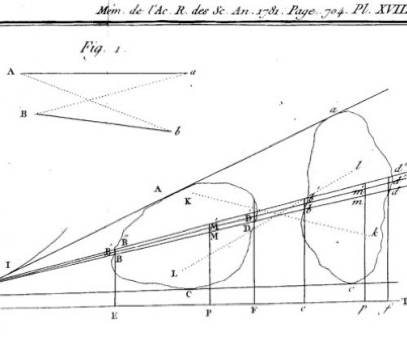
\includegraphics[width=.22\linewidth]{transport/monge-2d/article-monge}&
%        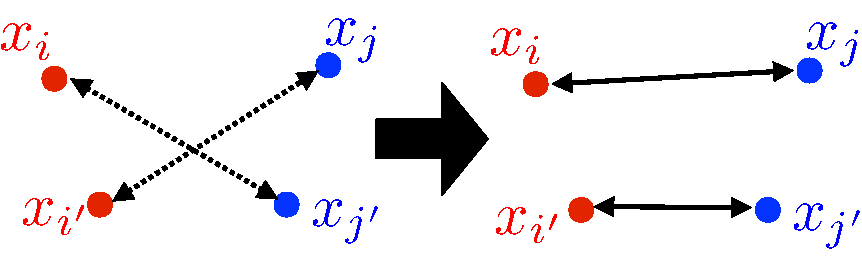
\includegraphics[width=.22\linewidth]{transport/monge-2d/decroisement}&
        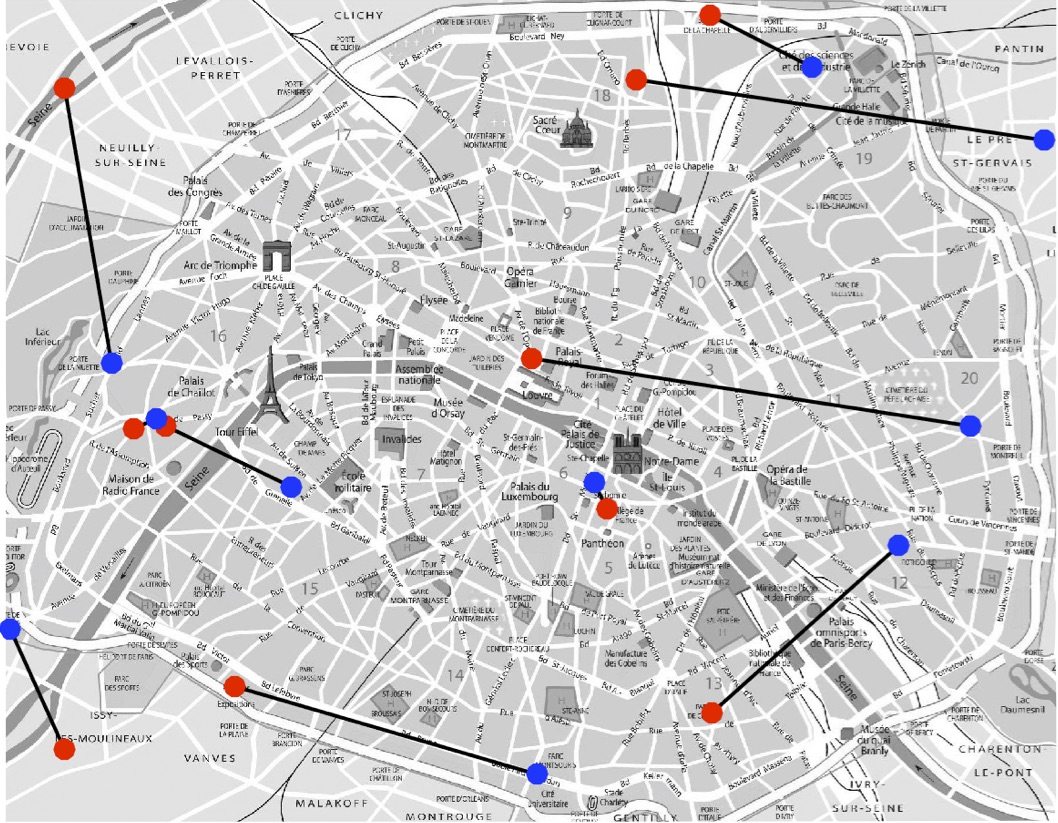
\includegraphics[width=.22\linewidth]{transport/monge-2d/example-10}&
        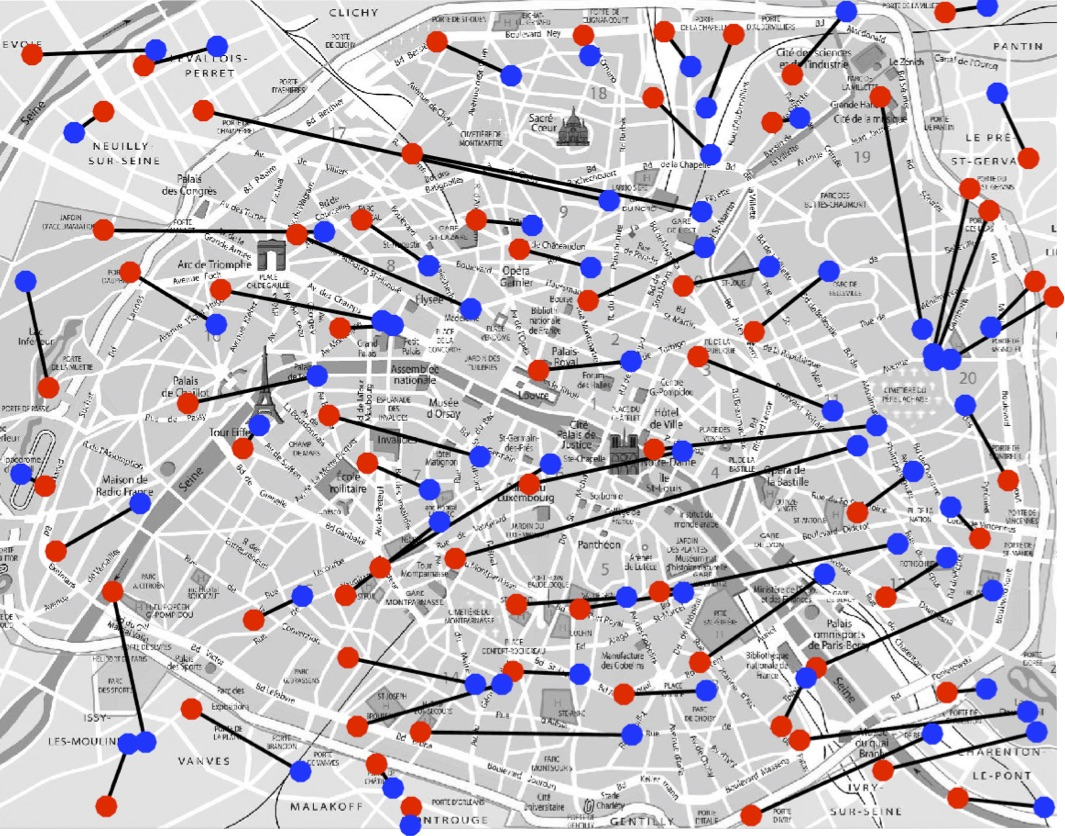
\includegraphics[width=.22\linewidth]{transport/monge-2d/example-70}
    \end{tabular}
    \caption{\label{fig:ot2d} Gauche: extrait de l'article de Monge~\cite{Monge1781}. Droite: le transport optimal en 2D pour un coût euclidien.  } 
\end{figure}

Cette observation géométrique n'est cependant pas suffisante pour calculer un transport optimal en 2D : il existe en effet beaucoup de permutations $\si$ telles que les segments associés ne se croisent pas. 
%
Il va falloir analyser de façon plus fine la structure des permutations optimales afin de pouvoir les calculer de façon efficace. 
%
Nous allons maintenant voir comment Leonid Kantorovitch a reformulé le problème de Monge afin d'y parvenir. 


%%%%%%%%%%%%%%%%%%%%%%%%%%%%%%%%%%%%%%%%%%%%%%
\section{Le Transport Optimal de Kantorovitch}
\label{sec-kanto}

Leonid Kantorovitch est un mathématicien et économiste soviétique qui a révolutionné la théorie du transport optimal pendant les années 40. Ses recherches sont issues de considérations pratiques qui l'ont occupé avant et après la seconde guerre mondiale. Il y a joué un rôle important pour assurer une distribution optimale des ressources, en particulier durant le siège de Léningrad.
%
Il a par la même occasion participé au développement de l'optimisation moderne, laquelle a eu un impact énorme dans de très nombreux domaines appliqués. Il a ainsi obtenu en 1975 le prix Nobel d'économie, car les premières applications (mais certainement pas les seules !) de sa théorie se sont manifestées dans ce domaine. 


%%%%%%%%%%%%%%%%%%%%%%%%%%%%%%%
\myparagraph{Le problème de Kantorovitch}

L'idée centrale de Kantorovitch~\cite{Kantorovich42} est de modifier le problème de Monge en remplaçant l'ensemble des permutations par un ensemble plus grand mais plus simple. Tout d'abord on remarque que l'on peut représenter une permutation $\si \in \Si_n$ à l'aide d'une matrice de permutation $P$ qui est une matrice binaire (remplie de 0 et de 1) de taille $n \times n$ telle que $P_{\iC,\jC} = 0$ sauf si $\jC=\si(\iC)$ auquel cas $P_{\iC,\si(\iC)} = 1$. Par exemple, pour $n=3$ points, les permutations 
$(\Red{1,2,3}) \mapsto (\Blu{1,2,3})$ (l'identité), 
$(\Red{1,2,3}) \mapsto (\Blu{3,2,1})$ et
$(\Red{1,2,3}) \mapsto (\Blu{2,1,3})$ sont respectivement représentées par les matrices de taille $3 \times 3$
\eq{
	\begin{pmatrix} 1&0&0 \\ 0&1&0 \\ 0&0&1 \end{pmatrix}, \quad
	\begin{pmatrix} 0&0&1 \\ 0&1&0 \\ 1&0&0 \end{pmatrix} \qetq
	\begin{pmatrix} 0&1&0 \\ 1&0&0 \\ 0&0&1 \end{pmatrix}.
}
Dans la suite, on note $\Pp_n$ l'ensemble des $n!$ matrices de permutation de taille $n \times n$.

Comme la matrice est binaire, avec seulement $n$ éléments non nuls égaux à 1, on peut remplacer la somme de $n$ termes qui apparait dans $\text{Coût}(\si)$ défini en~\eqref{eq:cout} par une somme sur l'ensemble des $n \times n$ indices $(\iC,\jC)$, c'est-à-dire que si $P$ est la matrice de permutation associée à $\si$, on a 
\eq{
	\text{Coût}(\si) = \sum_{\iC=1}^n \sum_{\jC=1}^n P_{\iC,\jC} C_{\iC,\jC}.
}
On peut ainsi remplacer le problème de Monge~\eqref{eq:monge} par le problème équivalent 
\eql{\label{eq:mongematrix}
    \umin{P \in \Pp_n}  \sum_{\iC=1}^n \sum_{\jC=1}^n P_{\iC,\jC} C_{\iC,\jC}.
}

Le génie de Kantorovitch a été de remarquer que l'on peut remplacer l'ensemble discret $\Pp_n$ (c'est-à-dire composé d'un ensemble fini, mais très grand, de $n!$ matrices) par un ensemble \guill{continu} (donc en particulier infini) mais plus simple. On remarque en effet que les matrices de permutation de $\Pp_n$ sont exactement les matrices qui ont un et un seul 1 le long de chaque ligne et de chaque colonne. Ceci peut aussi s'exprimer comme le fait qu'une matrice de permutation est une matrice binaire dont la somme de chaque ligne et de chaque colonne vaut 1, c'est-à-dire
\eq{
	\Pp_n = \enscond{ P \in \{0,1\}^{n \times n} }{ \foralls \iC, \sum_{\jC} P_{\iC,\jC}=1, \foralls \jC, \sum_{\iC} P_{\iC,\jC}=1  }.
}
Ce qui rend cet ensemble très compliqué, c'est la contrainte binaire, c'est-à-dire que ces matrices sont contraintes à être dans $\{0,1\}^{n \times n}$. Kantorovitch propose alors de \guill{relaxer} cette contrainte en supposant simplement que les entrées de $P$ sont entre $0$ et $1$. Ceci définit un ensemble plus grand, l'ensemble des matrices bistochastiques 
\eql{\label{eq:bistoch}
	\Bb_n \eqdef \enscond{ P \in [0,1]^{n \times n} }{ \foralls \iC, \sum_{\jC} P_{\iC,\jC}=1, \foralls \jC, \sum_{\iC} P_{\iC,\jC}=1  }.
}
Le problème de Kantorovitch s'obtient en effectuant ce remplacement dans~\eqref{eq:mongematrix}, afin de résoudre 
\eql{\label{eq:kantoassign}
    \umin{P \in \Bb_n} 
        \sum_{\iC=1}^n \sum_{\jC=1}^n P_{\iC,\jC} C_{\iC,\jC}.
}
L'immense avantage du problème de Kantorovitch~\eqref{eq:kantoassign} par rapport à celui de Monge~\eqref{eq:mongematrix} est que l'ensemble des matrices bistochastique est convexe, c'est-à-dire que si l'on considère deux matrices bistochastiques $P,Q \in \Bb_n$, alors leur moyenne $\frac{P+Q}{2} \in \Bb_n$ est encore bistochastique. Ceci n'est pas vrai pour les matrices de permutation, puisque la moyenne de deux matrices binaires $(P,Q)$ n'est pas binaire (sauf bien sûr si $P=Q$). Cette convexité est la clef pour le développement d'algorithmes efficaces. 
%
Cette nouvelle formulation a en effet pu bénéficier d'une deuxième révolution initiée par George Dantzig~\cite{Dantzig51}, qui, à la même époque, a proposé l'algorithme du simplexe. Celui-ci permet de résoudre efficacement une certaine classe de problèmes d'optimisation convexe : les problèmes de programmation linéaire, dont~\eqref{eq:kantoassign} est un cas particulier. Dans le cas du problème de Kantorovitch, il existe en effet un algorithme du simplexe qui a une complexité de l'ordre de $n^3$ opérations, ce qui permet de faire des calculs pour de grands $n$, de l'ordre de plusieurs milliers. 


%%%%%%%%%%%%%%%%%%%%%%%%%%%%%%%
\myparagraph{L'équivalence Monge--Kantorovitch}

L'ensemble des matrices bistochastiques est plus grand que celui des matrices de permutations, $\Pp_n \subset \Bb_n$, de sorte que l'on a l'inégalité 
\eql{\label{eq:monge-vs-kanto}
    \umin{P \in \Bb_n} 
        \sum_{\iC=1}^n \sum_{\jC=1}^n P_{\iC,\jC} C_{\iC,\jC}
     \leq 
    \umin{P \in \Pp_n} 
        \sum_{\iC=1}^n \sum_{\jC=1}^n P_{\iC,\jC} C_{\iC,\jC}
}
entre les problèmes de Kantorovitch et de Monge. Mais de façon à première vue surprenante, un théorème fondamental dû à George Birkhoff et à John von Neumann~\cite{birkhoff,von1953certain} assure qu'en fait il y a égalité entre les valeurs de ces deux minimisations. En effet, ce théorème montre qu'il existe toujours une matrice solution du problème de Kantorovitch qui est une matrice de permutation, de sorte qu'elle est aussi solution du problème de Monge. Attention cependant, en général il n'y a pas unicité des solutions de ces problèmes : il peut exister une matrice bistochastique solution du problème de Kantorovitch qui n'est pas une permutation. 
%
La conjonction de deux avancées spectaculaires, dues à Kantorovitch et à Dantzig, a permis de rendre le transport optimal applicable à des problèmes de grande taille, puisque l'algorithme du simplexe permet de résoudre en pratique ces problèmes. 

%%%%%%%%%%%%%%%%%%%%%%%%%%%%%%%
\myparagraph{Le cas pondéré}

Outre son intérêt pratique, la formulation de Kantorovitch a aussi permis de généraliser le problème initial de Monge, en donnant le bon cadre pour le formaliser et l'étudier mathématiquement. En effet, le problème de Monge est très limité. Que se passe-t-il par exemple s'il n'y pas le même nombre $n$ de cafés et $m$ de boulangeries ? Le problème initial~\eqref{eq:monge} n'a pas de solution, car on ne peut pas mettre en bijection deux ensembles de tailles différentes. Le bon concept n'est pas le nombre de boulangeries et de cafés, mais plutôt les distributions $(\Red{a_1,\ldots,a_n})$ de production (associées au boulangeries) et les distributions $(\Blu{b_1,\ldots,b_m})$ de consommation des cafés. 
%
Par exemple, si la première boulangerie produit 45 croissants par jour, on prendra $\Red{a_1} =45$, de même $\Blu{b_3} = 34$ signifie que le 3$^\text{e}$ café consomme 34 croissants par jour.
%
Dans le cas initialement considéré, où $n=m$, toutes les quantités $\Red{a_i}$ et $\Blu{b_j}$ sont égales à 1. Mais dans de nombreux cas concrets, ces quantités sont quelconques. Ces quantités doivent être positives, et vérifier 
\eq{
	\Red{a_1+\cdots+a_n} = \Blu{b_1 + \cdots + b_m}, 
}
de sorte qu'il y ait autant de production que de consommation. La construction de Kantorovitch s'adapte naturellement à ce cas de distributions générales, en remplaçant les matrices bistochastiques~\eqref{eq:bistoch} par des matrices de \guill{couplage} qui satisfont la contrainte de conservation de la masse 
\eq{
	\Bb(\aC,\bC) \eqdef \enscond{ P \in \RR_+^{n \times m} }{ \foralls \iC, \sum_{\jC} P_{\iC,\jC}=\Red{a_i}, \foralls \jC, \sum_{\iC} P_{\iC,\jC}= \Blu{b_j}  }.
}
Dans le cas initial où $n=m$ et $\Red{a_i}=\Blu{b_j}=1$, alors $\Bb(\aC,\bC) = \Bb_n$ et l'on retrouve des matrices bistochastiques. Dans le cas général, à chaque fois qu'une entrée $P_{\iC,\jC}$ est non-nulle, ceci signifie que l'on transfère de la \guill{masse} (ici une certaine quantité de croissants) entre $\iC$ et $\jC$. Comme le montre la figure~\ref{fig:coupling-visu}, on peut visualiser de différentes façons une telle matrice $P$ couplant deux distributions $(\aC,\bC)$.
%
Contrairement au cas des matrices bistochastiques, pour lequel il y a toujours une solution qui est une permutation, ici un couplage optimal $\Bb(\aC,\bC)$ peut avoir plus d'une seule entrée non-nulle $P_{\iC,\jC}$ le long d'une ligne indexée par $\iC$ (voir la figure~\ref{fig:coupling-visu}). Ceci signifie que cette boulangerie $\iC$ est connectée à plusieurs cafés, de sorte que sa production est alors séparée en plusieurs lots de croissants distribués, tout en satisfaisant la contrainte de conservation de la masse $\sum_{\jC} P_{\iC,\jC}=\Red{a_i}$.

\begin{figure}\centering
    \begin{tabular}{@{}c@{\hspace{1mm}}c@{\hspace{1mm}}c@{\hspace{1mm}}c@{}}
        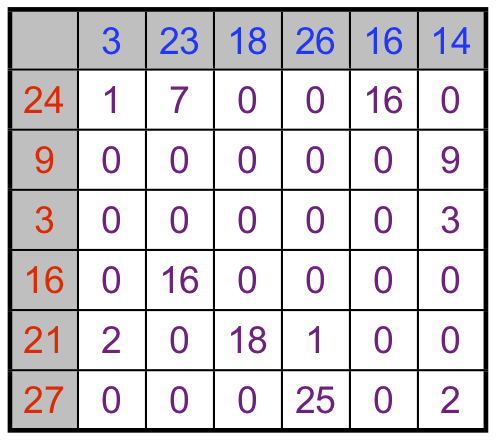
\includegraphics[width=.22\linewidth]{transport/kantorovitch/coupling-array}&
        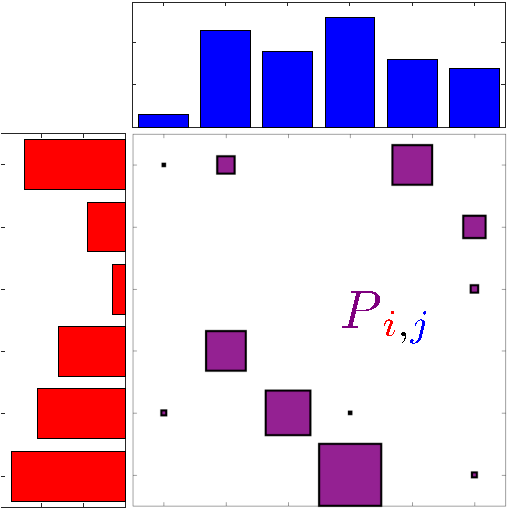
\includegraphics[width=.22\linewidth]{transport/kantorovitch/coupling-squares}&
        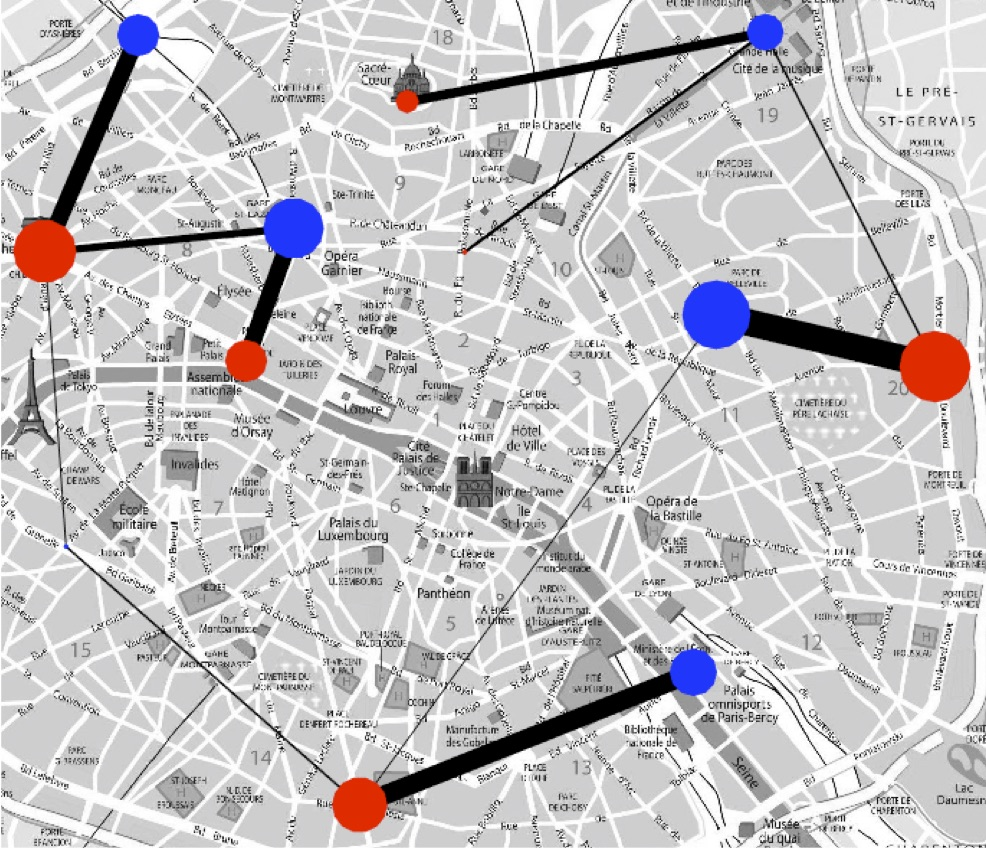
\includegraphics[width=.22\linewidth]{transport/kantorovitch/coupling-map}&
        \includegraphics[width=.22\linewidth]{transport/kantorovitch/coupling-bipartite} \\
        (a) matrice & (b) histogrammes & (c) segments & (d) graphe biparti
    \end{tabular}
    \caption{\label{fig:coupling-visu} Différentes façons de représenter une matrice de couplage $P \in \Bb(\aC,\bC)$:
    	(a) un tableau de nombres dont les lignes et colonnes ont des sommes prescrites ; 
		(b) un histogramme bidimensionnel dont la taille de carré est proportionnelle à $P_{\iC,\jC}$ ; 
		(c) un ensemble de segments dont la largeur est proportionnelle à $P_{\iC,\jC}$. 
		(d) un graphe biparti, c'est-à-dire avec deux groupes de points reliés par des arêtes.   } 
\end{figure}


Le problème de Kantorovitch qui généralise~\eqref{eq:kantoassign} s'écrit alors
\eql{\label{eq-kanto-gen}
    \umin{P \in \Bb(\aC,\bC)} 
        \sum_{\iC=1}^n \sum_{\jC=1}^m P_{\iC,\jC} C_{\iC,\jC}
}
ce qui signifie que l'on doit payer un coût  $C_{\iC,\jC}$ à chaque fois que l'on transfère une unité de masse entre $\iC$ et $\jC$. Tout comme le problème original~\eqref{eq:kantoassign}, on peut le résoudre de façon efficace avec l'algorithme du simplexe.  La figure~\ref{fig:coupling-visu} montre un exemple de couplage optimal. 



%%%%%%%%%%%%%%%%%%%%%%%%%%%%%%%%%%%%%%%%%%%%%%
\section{Les applications}

Bien que les motivations initiales de Monge et Kantorovitch aient été respectivement militaires et économiques, le transport optimal a trouvé d'innombrables applications, à la fois théoriques et concrètes. Sur le plan mathématique, on peut considérer des distributions \guill{continues} de masses, en quelque sorte la limite quand le nombre de points $n$ tend vers l'infini. Ceci permet de définir le problème de transport entre des mesures de probabilités quelconques. Ce point de vue théorique est extrêmement fructueux, et c'est le mathématicien français Yann Brenier qui a le premier montré l'équivalence dans le cadre continu des formulations de Monge et de Kantorovich~\cite{Brenier91}. Ces travaux pionniers ont montré la connexion entre le problème de transport et les équations aux dérivées partielles, et ont débouché, entre autres, sur les médailles Fields de Cédric Villani (2010) et Alessio Figalli (2018). 

\begin{figure}\centering
\begin{tabular}{@{}c@{\hspace{1mm}}c@{\hspace{1mm}}c@{}}
    \includegraphics[width=.24\linewidth]{transport/applis/painting-2} &
    \includegraphics[width=.24\linewidth]{transport/applis/painting-1} &
    \includegraphics[width=.24\linewidth]{transport/applis/painting-2-equalized} \\
    Image $(\Red{x_i})_{\iC=1}^n$ & Image $(\Blu{y_j})_{\jC=1}^n$ & Image  $(y_{\si(\iC)})_{\iC=1}^n$ \\
    \includegraphics[width=.24\linewidth]{transport/applis/painting-2-histo}&
    \includegraphics[width=.24\linewidth]{transport/applis/painting-1-histo}&
    \includegraphics[width=.24\linewidth]{transport/applis/painting-1-histo}
\end{tabular}
\caption{\label{fig:image-eq} Exemple de transfert de palettes de couleurs à l'aide du transport optimal. 
	Haut: les pixels sont sur la grille d'affichage pour former une image couleur. 	
	Bas: les pixels sont placés à leurs positions dans $\RR^3$ pour former un nuage de points. }
\end{figure}

Le transport optimal est depuis peu au c\oe{}ur de problématiques plus appliquées en sciences des données, en particulier pour résoudre des problèmes en traitement d'image et en apprentissage machine. 
%
La première idée, la plus immédiate, est d'utiliser la bijection $\si$ afin de transformer des données, par exemple des images. Dans ce cas, on considère les pixels $(\Red{x_i})_{\iC=1}^n$ et $(\Blu{y_j})_{\jC=1}^n$ de deux images couleur. Chaque pixel $\Red{x_i}, \Blu{y_j} \in \RR^3$ est un vecteur de dimension 3, qui représente les intensités de chacune des trois couleurs élémentaires, rouge, vert et bleu. Afin de changer les couleurs de la première image, et lui imposer la palette de la deuxième image, on calcule le transport $\si$ pour la matrice de coût $C_{\iC,\jC} = \norm{\Red{x_i} - \Blu{y_j}}^2$ (c'est-à-dire le carré de la norme euclidienne dans $\RR^3$), c'est-à-dire le carré de la distance euclidienne entre les pixels. L'image avec les couleurs modifiées est $(y_{\si(\iC)})_{\iC=1}^n$, c'est à dire que l'on remplace dans la première image le pixel $\Red{x_i}$ par le pixel $y_{\si(\iC)}$. Cette image ressemble à la première, mais a la palette de couleurs de la deuxième image.
%
La figure~\ref{fig:image-eq} illustre ce procédé pour imposer la palette de couleurs de Picasso à un tableau de Cézanne. 

On peut également utiliser le transport optimal pour des problèmes plus difficiles, en n'utilisant que de façon indirecte la bijection $\si$ ou bien la matrice de couplage optimal $P \in \Bb(\aC,\bC)$. L'idée centrale est que la quantité associée à un couplage optimal $P$ solution de~\eqref{eq-kanto-gen}
\eq{
	W(\aC,\bC) \eqdef \sum_{i,j} P_{\iC,\jC} C_{\iC,\jC}
}
définit en quelque sorte l'effort nécessaire pour déplacer la masse de la distribution $\aC$ vers la distribution $\bC$. Elle permet donc de quantifier combien ces deux distributions sont \guill{proches}. Par exemple, si $C_{\iC,\jC} = \norm{\Red{x_i} - \Blu{y_j}}^2$ est le carré de la distance euclidienne entre des points, alors la quantité $W(\aC,\bC)^{1/2}$ est une distance entre les distributions, en particulier elle vérifie $W(\aC,\bC)=0$ si et seulement si $\aC=\bC$, et elle vérifie l'inégalité triangulaire. Ces propriétés sont très importantes pour permettre d'appliquer le transport à des problèmes pratiques.


\begin{figure}\centering
        \includegraphics[width=.6\linewidth]{transport/applis/shapes-3d}
    \caption{\label{fig:barycenters} Exemple d'interpolation barycentrique entre des formes 3D, obtenu en minimisant~\eqref{eq-bary}.  }
\end{figure}

Un exemple typique d'application de cette quantité $W$ consiste à calculer des barycentres entre des distributions~\cite{agueh2011barycenters}. La figure~\ref{fig:barycenters} montre un exemple où l'on considère trois distributions $a,b,c$ (montrées aux trois sommets du triangles) qui sont des distributions uniformes de masse à l'intérieur de formes 3D (c'est-à-dire que la masse $a_i$ associée au $i^{\text{e}}$ point est 0 à l'extérieur de la première forme et prend une valeur constante à l'intérieur). 
%
On calcule un barycentre pondéré de ces trois distributions en imitant le fait que dans un espace Euclidien, le barycentre pondéré $r$ de trois points $x,y,z$ minimise la somme des distances au carré
\eq{
    \umin{r} \al \norm{x-r}^2 + \be \norm{y-r}^2 +  \ga \norm{z-r}^2,
}
où les poids $(\al,\be,\ga)$ sont les pondérations du barycentre, qui sont des réels positifs et tels que $\al+\be+\ga=1$.
%
Le barycentre pondéré $d$  de $(a,b,c)$ minimise ainsi la somme pondérée de distances de transport optimal
\eql{\label{eq-bary}
	\umin{d} \al W(a,d) + \be W(b,d) + \ga W(c,d).
}
En modifiant les poids $(\al,\be,\ga)$, on modifie la forme obtenue en se déplaçant à l'intérieur d'un triangle de transport optimal. 
%
On peut utiliser cette distance $W$ pour bien d'autres applications où l'on doit comparer des distributions de probabilité. C'est le cas en apprentissage machine, par exemple pour comparer des textes à l'aide des distributions des mots qui les composent. La figure~\ref{fig:bagwords} illustre les histogrammes d'apparition des mots pour deux textes, où la taille des lettres du mot $\iC$ est proportionnelle à la masse $\aC_\iC$. Une question difficile dans ce cas est de savoir quelle matrice de coût $C_{\iC,\jC}$ utiliser entre deux mots $(\iC,\jC)$. Il s'agit d'un travail de linguistique (caractériser la proximité sémantique entre des mots du langages), que l'on peut chercher à résoudre en même temps que le transport optimal~\cite{huang2016supervised}. 

\begin{figure}\centering
    \includegraphics[width=.35\linewidth]{transport/applis/bag-word-1}
    \qquad
    \includegraphics[width=.35\linewidth]{transport/applis/bag-word-2}
\caption{\label{fig:bagwords} Exemples d'histogrammes de distributions des mots, qui peuvent être utilisés pour comparer les discours d'Obama et de Lincoln (seuls les mots les plus fréquents sont montrés).  }
\end{figure}


%%%%%%%%%%%%%%%%%%%%%%%%%%%%%%%%%%%%%%%%%%%%%%
\section*{Conclusions}

Le transport optimal a connu de nombreuses révolutions. Sous l'impulsion de mathématiciens tels que Monge, Kantorovitch, Dantzig et Brenier, il est progressivement devenu un outil théorique et numérique fondamental. 
%
Il est maintenant au c\oe{}ur de questions importantes en science des données pour modéliser, résoudre numériquement et analyser théoriquement les problèmes de l'apprentissage machine. Les opportunités pour développer de nouvelles théories et des algorithmes performants sont immenses. 
%
Pour plus d'informations sur les aspects théoriques du transport optimal, on pourra consulter les livres~\cite{Villani03,SantambrogioBook}. Les aspects numériques et applicatifs sont couverts dans le livre~\cite{PeyreCuturi}.


%%%%%%%%%%%%%%%%%%%%%%%%%%%%%%%%%%%%%%%%%%%%%%
\section*{Remerciements}

Je tiens à remercier Vincent Beck, Gwenn Guichaoua et Marie-Noëlle Peyré pour leurs relectures attentives. 




\bibliographystyle{plain}
\bibliography{biblio-sparsity,biblio-shannon,biblio-ot}


\end{document}

